% This is a template for Ph.D. dissertations in the UCI format.
% 
% All fonts, including those for sub- and superscripts, must be 10
% points or larger.  Recommended sizes are 14-point for chapter
% headings, 12-point for the main body of text and figure/table
% titles, and 10-point for footnotes, sub- and super-scripts, and text
% in figures and tables.
%
% Notes: Add short title to figures, sections, via square brackets,
% e.g. \section[short]{long}.
%
\documentclass[12pt,fleqn]{ucithesis}

% A few common packages
\usepackage{amsmath}
\usepackage{amsthm}
\usepackage{array}
\usepackage{graphicx}
%\usepackage{natbib}
\usepackage{relsize}
\usepackage[T1]{fontenc}
% Some other useful packages
\usepackage{caption}
\usepackage{subcaption}  % \begin{subfigure}...\end{subfigure} within figure
\usepackage{multirow}
\usepackage{tabularx}
\usepackage{pdfpages}

% plainpages=false fixes the "duplicate ignored" error with page counters
% Set pdfborder to 0 0 0 to disable colored borders around PDF hyperlinks
\usepackage[plainpages=false,pdfborder={0 0 0}]{hyperref}




\DeclareGraphicsExtensions{.pdf,.png,.jpg}
\usepackage{setspace}
\usepackage[english]{babel}
\usepackage[semicolon,round]{natbib} %separates each citation by a comma
%\usepackage[numbers]{natbib} %uses numbers instead of text
%\setcitestyle{notesep={:}} %page number separator is semicolon instead of a comma
%\usepackage{url}
\usepackage{ulem} % when using ulem package, must change \emph to \it for italics.
%\usepackage[colorlinks,citecolor=blue,urlcolor=blue,linkcolor=black]{hyperref} %hyperref package, also colorlinks and citecolor adds colored citations to text. urlcolor adds colored urls to text, linkcolor changes colors of footnotes.
\usepackage{amssymb,amsmath,tabu}
\usepackage{dcolumn}%for stata to LaTeX column alignment for tables.
%\usepackage{booktabs}%for stata to LaTeX vertical spacing (between hlines and coefficients) alignment for tables.
\usepackage{wrapfig}
\usepackage{lscape}
\usepackage{longtable}
\usepackage{rotating}
\usepackage{epstopdf}
\usepackage{booktabs}
%\usepackage[]{figcaps}
%\usepackage{hanging}
%\usepackage[margin=1.0in]{geometry}
%\usepackage{authblk} %package for blocking authors, followed by blocking affiliation
%\usepackage{indentfirst}
%\usepackage{ragged2e}
%\usepackage{tabularx}
\usepackage{ltablex}
\usepackage{ltxtable}
\usepackage[super]{nth}
\usepackage{pdflscape}%landscape pages
%\usepackage[singlelinecheck=false]{caption} % this left aligns the Table name/caption
%\usepackage[justification=justified,singlelinecheck=false]{caption}
\newcommand{\ccc}[1]{\citep{#1}} %use this to make a new citealt or any other command
%\usepackage[T1]{fontenc} %add encoding for small caps
%\newlength{\saveparindent} %allows you to use \RaggedRight with paragraph indents below
%\setlength{\saveparindent}{\parindent}%allows you to use \RaggedRight with paragraph indents below
%\raggedright%allows you to use \RaggedRight with paragraph indents below
%\setlength{\parindent}{\saveparindent}%allows you to use \RaggedRight with paragraph indents below
\usepackage{etoolbox}
%\usepackage[figures,tables]{endfloat}
\urlstyle{same}%keeps url font the same LaTeX font, and not fixed width/courier new
%\usepackage[singlelinecheck=false]{caption} % this left aligns the Table name/caption
%\usepackage[justification=justified,singlelinecheck=false]{caption}

%\usepackage{endnotes} %endnotes instead of footnotes

%\let\footnote=\endnote %endnotes instead of footnotes


% Uncomment the following two lines to use the algorithm package,
% which provides an algorithm environment similar to figure and table
% ("\begin{algorithm}...\end{algorithm}"). A list of algorithms will
% automatically be added in the preliminary pages. Note that you
% probably want a package for the actual code to go with this (e.g.,
% algorithmic).
%\usepackage{algorithm}
%\renewcommand{\listalgorithmname}{\protect\centering\protect\Large LIST OF ALGORITHMS}

% Uncomment the following line to enable Unicode support. This will allow you
% to enter non-ASCII characters (such as accented characters) directly without
% having to use LaTeX's awkward escape syntax (e.g., \'{e})
% NOTE: You may have to install the ucs.sty package for this to work. See:
% http://www.unruh.de/DniQ/latex/unicode/
%\usepackage[utf8x]{inputenc}

% Uncomment the following to avoid "widowing", where page breaks cause
% single lines of paragraphs to float onto the next page (this is not
% a UCI requirement but more of an aesthetic choice).
%\widowpenalty=10000
%\clubpenalty=10000

% Modify or extend these at will.
\newtheorem{theorem}{\textsc{Theorem}}[chapter]
\newtheorem{definition}{\textsc{Definition}}[chapter]
\newtheorem{example}{\textsc{Example}}[chapter]

% Macros for title, author, abstract, etc.

\thesistitle{The Evolution of Marijuana Politics in the United States}

%"Dissertation" for PhD, "Thesis" for master's
\documenttitle{Dissertation}

\degreename{Doctor of Philosophy}

% Use the wording given in the official list of degrees awarded by UCI:
% http://www.rgs.uci.edu/grad/academic/degrees_offered.htm
\degreefield{Sociology}

% Your name as it appears on official UCI records.
\authorname{Burrel James Vann Jr}

% Use the full name of each committee member.
\committeechair{Edwin Amenta}
\othercommitteemembers
{
  David S. Meyer\\
  Charles Ragin\\
  Rory McVeigh
}

\degreeyear{2019}

\copyrightdeclaration
{
  {\copyright} {\Degreeyear} \Authorname
}

% If you have previously published parts of your manuscript, you must list the
% copyright holders; see Section 3.2 of the UCI Thesis and Dissertation Manual.
% Otherwise, this section may be omitted.
% \prepublishedcopyrightdeclaration
% {
% 	Chapter 4 {\copyright} 2003 Springer-Verlag \\
% 	Portion of Chapter 5 {\copyright} 1999 John Wiley \& Sons, Inc. \\
% 	All other materials {\copyright} {\Degreeyear} \Authorname
% }

% The dedication page is optional
% (comment out to exclude).
\dedications
{
  To my communities...
}

\acknowledgments
{
  I would like to thank numerous individuals and organizations, without whom this dissertation would not have been possible. 
  
  I am grateful to my advisors and committee: Edwin Amenta, David Meyer, Rory McVeigh, and Charles Ragin for their mentorship, support, and sage advice on this and other projects over the years. 
  
   I would like to thank those shadow advisors who, oftentimes, aren't given the credit they deserve. It is for this reason I would like to thank Davin Phoenix -- without whom I would likely not have a job, and Christopher Parker, who has served nothing but realness and support during my graduate school career. As people of color, I am grateful for your support and mentorship. 
  
  
  %I am grateful to Edwin Amenta, whose advisement steered the direction of this work. I am also thankful for David Meyer, who, even before graduate school was willing to help me devise good research projects, while also caring about my wellbeing. Finally, I would like to thank Rory McVeigh, whose guidance, advice, mentorship, and work has heavily influenced this work. 
  
  I would like to thank faculty at the University of California, Irvine who have provided feedback and support along the way, including Evan Schofer, Nina Bandelj, Carter Butts, John Hipp, David Snow, Yang Su, Andrew Noymer, Sabrina Strings, Rocio Rosales, Jacob Avery, Katie Bolzendahl, and Katie Faust. In addition, I would like to thank the staff who've made my time at Irvine seamless, including John Sommerhauser, Ekua Arhin, Maryann Zovak-Wieder, and Hannah Absher.
  
  Of course, I cannot forget my UCI student life family. These people have been critical to my success and sanity during graduate school. I would like to thank Mart\'{i}n Jacinto, Miles Davison, Jess Lee, Sara Villalta, Claudia Campos, Alma Garza, Monique Kelly, Dana Moss, Thomas Elliott, Amber Tierney, Eulalie Laschever, Jonathan Lui, Kara Placek, Ksenia Gracheva, Ted Watson, John McCollum, Bonnie Bui, Jessica Kizer, Connor Strobel, Chris Gibson, Aaron Tester, Katt Hoban, Steph Jones, Mariam Ashtiani, Alice Motes, Dana Nakano, Hector Y. Martinez, Matt Rafalow, Nolan Phillips, Jayson Hunt, and Tyson Patros. In addition, I would like to thank those amazing friends in my cohort: Emma Smith, Sean Drake, Tanya Sanabria, Chris Zoeller, Zaib Tufail, and David Kong. Importantly, my life would have not been the same without the intellect, wit, skills, and connections with my good friends Rodolfo Lopez and Ben Gibson. I am truly grateful for their friendship. 
  
  In 2011, I was lucky enough to conduct research at the University of Notre Dame. During that Summer, and throughout the next year, I was able to develop strong relationships with many people. For their wisdom and friendship, I would like to thank Bryant Crubaugh, San Diego-native Austin Choi-Fitzpatrick, (brother) Jeffrey Seymour, David Everson, Marshall Taylor, Kevin Estep, Heather Price, Peter Barwis, Kristi Donaldson, Jonathan Schwarz, Nicole Perez, Ana Velitchkova, Ellen Childs, Josh Dinsman, Amy Jonason, Jade Avelis, Linda Kawentel, Megan Rogers, Megan Austin, and Matthew Chandler. Most importantly, I am so appreciative of my dude... my co-metalcorehead/co-insert-subgenre-here-head/$\emptyset$ fam, Justin Van Ness. Over the years, we've crashed on each other's couches, gone to shows, explored cities, eaten good food, suggested new bands, tried out new breweries, and rocked tf out together, while being professional by presenting our work at conferences, networking, and crankin' papes. Cheers to keeping it strong for many years to come.
  
I am grateful for my Ford Foundation family, which has been integral to my success. Without them, I would not be where I am today. A huge reason why I persisted in graduate school was because of these people. I am truly appreciative of these people of color. I would like to thank the people who stayed so close despite our distance: Victor Ray, Piko Ewoodzie, and Anthony Ocampo. These three have only been a text/phone call away. I am also grateful for so many others in my Ford family, including Vanessa D\'{i}az, Elliott Powell, Jonathan Rosa, Elizabeth Hinton, Yasmiyn Irizarry, Rashwan Ray, Abigail ``Aly'' Sewell, Augustin Diaz, Vlad Medenica, and Armand Gutierrez. 
  
 I would like to give a shout out to all the musicians and artists whose work kept me motivated to complete this work. Most of all, Architects, which has consistently provided heavy, politically-motivated music throughout my graduate career. I am also thankful for music created by letlive., Bring Me the Horizon (2004-2013), The Devil Wears Prada (2005-2010), Drop Dead Gorgeous, Dance Gavin Dance, Chelsea Grin (2018), Kendrick Lamar, Saosin, Lions Lions, Wind in Sails, Vanna (2004-2010), Jamie's Elsewhere, Pierce the Veil, Before Today, and Four Year Strong. 
  
 % My Family:
   I would also like to thank those people who have shaped me into the person I am, but may not recognize their impact. First, I would like to thank my closest friends from when I was a music major during my undergraduate career, including Loren Gamarra and John Urban. It was difficult to transition out of music, but I think I made a good choice. In addition, I would like to thank my brothers Joe Salcido, Reginald Webber Jr., Javier, Mike Ouellet, Kirshon Asborno, Jesse Glick, Matt McDavid, Chris Benzen, Jon Keith, Ib Salleh, Ish Salleh, other brothers Owen Griffin, Chad Morris, and Jon Locke, and (of course) my littles -- Alison Bellman and Derek Dobbs. 
   
   I chose to move on from a degree in music to a degree in sociology, in part, because of the inequality experiences shared by my fellow musician friends. I would like to thank Sean Murillo, John Whitt Jr., and all those others from the Tulare Western High School Drumline, and Band \& Colorguard.  %I am also thankful for those who helped me sustain my passion in music, including Raymond Ferenci, Matt Boyett, Darren Suey, Yolanda Flores, Nick Perry, Chris Ramos, Brian Frasquillo, Johanna Ilano, Jonathan Victorino, Richard Vowell, and Darcy XXX and many others from Tulare Western High School who shaped me. 
   I would like to also thank Michaela and Talina, and all the members of the innercircle: David Scott (TEDS), Brandon Lee Taylor (RANDO), and Jordan Aguirre (NADROJ). To you all, I say: LPCG. 
   
  
  I would also like to thank the Ford Foundation for funding earlier versions of this project through the Predoctoral Fellowship and the Dissertation Fellowship. 
  
}


% Some custom commands for your list of publications and software.
%\newcommand{\mypubentry}[3]{
%  \begin{tabular*}{1\textwidth}{@{\extracolsep{\fill}}p{4.5in}r}
%    \textbf{#1} & \textbf{#2} \\ 
%    \multicolumn{2}{@{\extracolsep{\fill}}p{.95\textwidth}}{#3}\vspace{6pt} \\
%  \end{tabular*}
%}
%\newcommand{\mysoftentry}[3]{
%  \begin{tabular*}{1\textwidth}{@{\extracolsep{\fill}}lr}
%    \textbf{#1} & \url{#2} \\
%    \multicolumn{2}{@{\extracolsep{\fill}}p{.95\textwidth}}
%    {\emph{#3}}\vspace{-6pt} \\
%  \end{tabular*}
%}

% Include, at minimum, a listing of your degrees and educational
% achievements with dates and the school where the degrees were
% earned. This should include the degree currently being
% attained. Other than that it's mostly up to you what to include here
% and how to format it, below is just an example.
%
% CV is required for PhD theses, but not Master's
% comment out to exclude
\curriculumvitae
{
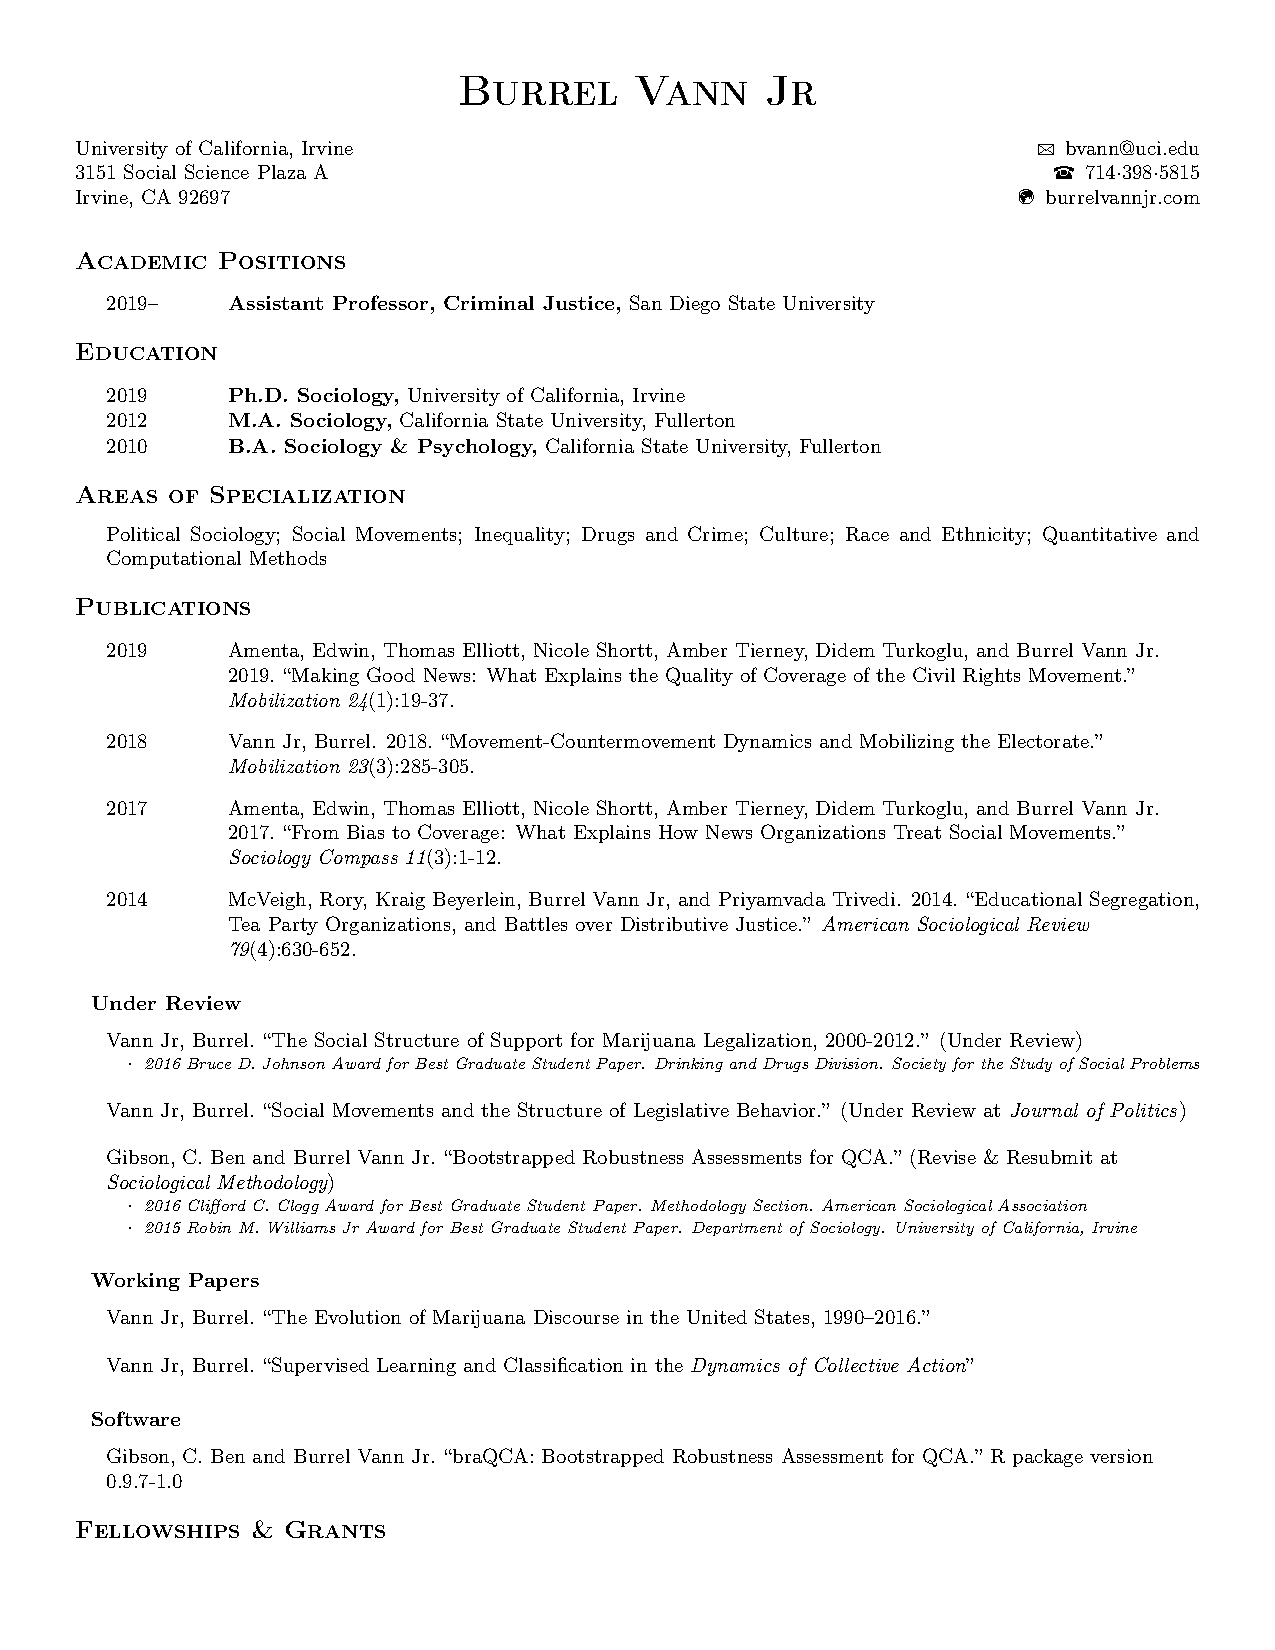
\includepdf[pages=-,pagecommand={}]{cv.pdf}
%\textbf{EDUCATION}
  
%  \begin{tabular*}{1\textwidth}{@{\extracolsep{\fill}}lr}
%    \textbf{Doctor of Philosophy in Computer Science} & \textbf{2012} \\
%    \vspace{6pt}
%    University name & \emph{City, State} \\
%    \textbf{Bachelor of Science in Computational Sciences} & \textbf{2007} \\
%    \vspace{6pt}
%    Another university name & \emph{City, State} \\
%  \end{tabular*}

%\vspace{12pt}
%\textbf{RESEARCH EXPERIENCE}

%  \begin{tabular*}{1\textwidth}{@{\extracolsep{\fill}}lr}
%    \textbf{Graduate Research Assistant} & \textbf{2007--2012} \\
%    \vspace{6pt}
%    University of California, Irvine & \emph{Irvine, California} \\
%  \end{tabular*}

%\vspace{12pt}
%\textbf{TEACHING EXPERIENCE}

%  \begin{tabular*}{1\textwidth}{@{\extracolsep{\fill}}lr}
%    \textbf{Teaching Assistant} & \textbf{2009--2010} \\
%    \vspace{6pt}
%    University name & \emph{City, State} \\
%  \end{tabular*}

%\pagebreak

%\textbf{REFEREED JOURNAL PUBLICATIONS}

%  \mypubentry{Ground-breaking article}{2012}{Journal name}

%\vspace{12pt}
%\textbf{REFEREED CONFERENCE PUBLICATIONS}

%  \mypubentry{Awesome paper}{Jun 2011}{Conference name}
%  \mypubentry{Another awesome paper}{Aug 2012}{Conference name}

%\vspace{12pt}
%\textbf{SOFTWARE}

%  \mysoftentry{Magical tool}{http://your.url.here/}
%  {C++ algorithm that solves TSP in polynomial time.}

}




%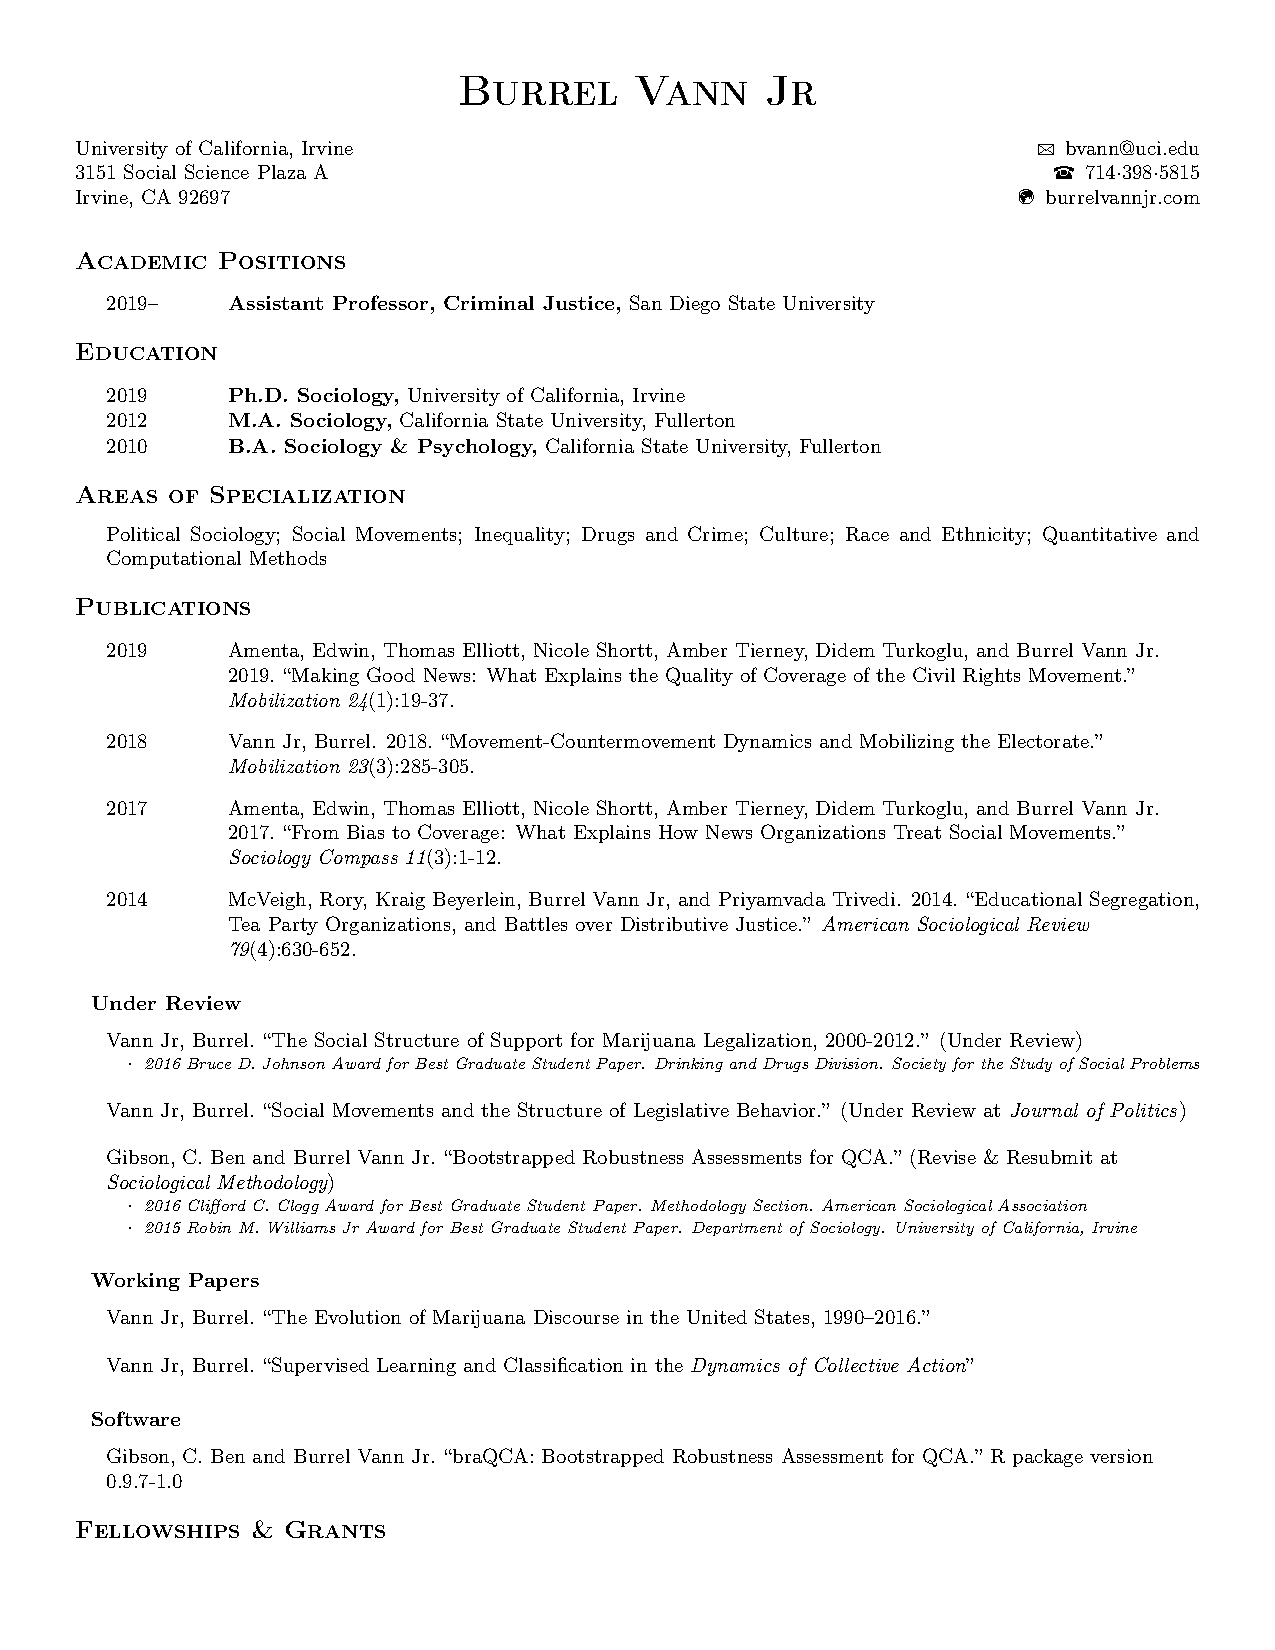
\includepdf[pages=1-]{cv.pdf}

% The abstract was previously limited to a maximum of 350 words, 
% but the UCI manual at https://etd.lib.uci.edu/electronic/td2e#2.2.1.
% currently does not indicate that there is any word limit for the abstract
\thesisabstract
{
  %In the absence of comprehensive drug policy reform or political advocates, states and counties have become venues for policy change. 
  This dissertation investigates the causes of support for marijuana legalization across the United States. Across three empirical studies, I argue that increased support for and passage of legalization resulted from 1) increased attention to marijuana, and shifting frames associated with marijuana combined with 2) structural and political conditions that allowed for the resonance of claims about the benefits of marijuana legalization. The first study explores the dramatic shift in coverage of marijuana from 1990 to 2016. I show that media coverage of marijuana shifted from from dominant negative narratives of criminality and delinquency to more neutral coverage, focusing on revenue creation and linking marijuana to political behavior. The second study links discursive data to public opinion, structural, and political environment data to show that the shift towards positive discourse about marijuana was significantly associated with a quicker pace of legalization across the United States. In the final study, an analysis of marijuana legalization ballot initiatives, I find that counties with high levels of parental segregation have higher levels of support for legalization. This dissertation reveals a less understood mechanism of the policymaking process: when political advocates are lacking, the strategic use of media can transform meanings associated with contentious issues and garner public support. 
}


%%% Local Variables: ***
%%% mode: latex ***
%%% TeX-master: "thesis.tex" ***
%%% End: ***

%
\thesistitle{The Evolution of Marijuana Politics in the United States}

%"Dissertation" for PhD, "Thesis" for master's
\documenttitle{Dissertation}

\degreename{Doctor of Philosophy}

% Use the wording given in the official list of degrees awarded by UCI:
% http://www.rgs.uci.edu/grad/academic/degrees_offered.htm
\degreefield{Sociology}

% Your name as it appears on official UCI records.
\authorname{Burrel James Vann Jr}

% Use the full name of each committee member.
\committeechair{Edwin Amenta}
\othercommitteemembers
{
  David S. Meyer\\
  Charles Ragin\\
  Rory McVeigh
}

\degreeyear{2019}

\copyrightdeclaration
{
  {\copyright} {\Degreeyear} \Authorname
}

% If you have previously published parts of your manuscript, you must list the
% copyright holders; see Section 3.2 of the UCI Thesis and Dissertation Manual.
% Otherwise, this section may be omitted.
% \prepublishedcopyrightdeclaration
% {
% 	Chapter 4 {\copyright} 2003 Springer-Verlag \\
% 	Portion of Chapter 5 {\copyright} 1999 John Wiley \& Sons, Inc. \\
% 	All other materials {\copyright} {\Degreeyear} \Authorname
% }

% The dedication page is optional
% (comment out to exclude).
\dedications
{
  (Optional dedication page)
  
  To ...
}

\acknowledgments
{
  I would like to thank...
  
  (You must acknowledge grants and other funding assistance. 
  
  You may also acknowledge the contributions of professors and
  friends.
  
  You also need to acknowledge any publishers of your previous
  work who have given you permission to incorporate that work
  into your dissertation. See Section 3.2 of the UCI Thesis and
  Dissertation Manual.)
}


% Some custom commands for your list of publications and software.
%\newcommand{\mypubentry}[3]{
%  \begin{tabular*}{1\textwidth}{@{\extracolsep{\fill}}p{4.5in}r}
%    \textbf{#1} & \textbf{#2} \\ 
%    \multicolumn{2}{@{\extracolsep{\fill}}p{.95\textwidth}}{#3}\vspace{6pt} \\
%  \end{tabular*}
%}
%\newcommand{\mysoftentry}[3]{
%  \begin{tabular*}{1\textwidth}{@{\extracolsep{\fill}}lr}
%    \textbf{#1} & \url{#2} \\
%    \multicolumn{2}{@{\extracolsep{\fill}}p{.95\textwidth}}
%    {\emph{#3}}\vspace{-6pt} \\
%  \end{tabular*}
%}

% Include, at minimum, a listing of your degrees and educational
% achievements with dates and the school where the degrees were
% earned. This should include the degree currently being
% attained. Other than that it's mostly up to you what to include here
% and how to format it, below is just an example.
%
% CV is required for PhD theses, but not Master's
% comment out to exclude
%\curriculumvitae
%{

%\textbf{EDUCATION}
  
%  \begin{tabular*}{1\textwidth}{@{\extracolsep{\fill}}lr}
%    \textbf{Doctor of Philosophy in Computer Science} & \textbf{2012} \\
%    \vspace{6pt}
%    University name & \emph{City, State} \\
%    \textbf{Bachelor of Science in Computational Sciences} & \textbf{2007} \\
%    \vspace{6pt}
%    Another university name & \emph{City, State} \\
%  \end{tabular*}

%\vspace{12pt}
%\textbf{RESEARCH EXPERIENCE}

%  \begin{tabular*}{1\textwidth}{@{\extracolsep{\fill}}lr}
%    \textbf{Graduate Research Assistant} & \textbf{2007--2012} \\
%    \vspace{6pt}
%    University of California, Irvine & \emph{Irvine, California} \\
%  \end{tabular*}

%\vspace{12pt}
%\textbf{TEACHING EXPERIENCE}

%  \begin{tabular*}{1\textwidth}{@{\extracolsep{\fill}}lr}
%    \textbf{Teaching Assistant} & \textbf{2009--2010} \\
%    \vspace{6pt}
%    University name & \emph{City, State} \\
%  \end{tabular*}

%\pagebreak

%\textbf{REFEREED JOURNAL PUBLICATIONS}

%  \mypubentry{Ground-breaking article}{2012}{Journal name}

%\vspace{12pt}
%\textbf{REFEREED CONFERENCE PUBLICATIONS}

%  \mypubentry{Awesome paper}{Jun 2011}{Conference name}
%  \mypubentry{Another awesome paper}{Aug 2012}{Conference name}

%\vspace{12pt}
%\textbf{SOFTWARE}

%  \mysoftentry{Magical tool}{http://your.url.here/}
%  {C++ algorithm that solves TSP in polynomial time.}

%}




%%% Local Variables: ***
%%% mode: latex ***
%%% TeX-master: "thesis.tex" ***
%%% End: ***

%\usepackage{pdfpages}
%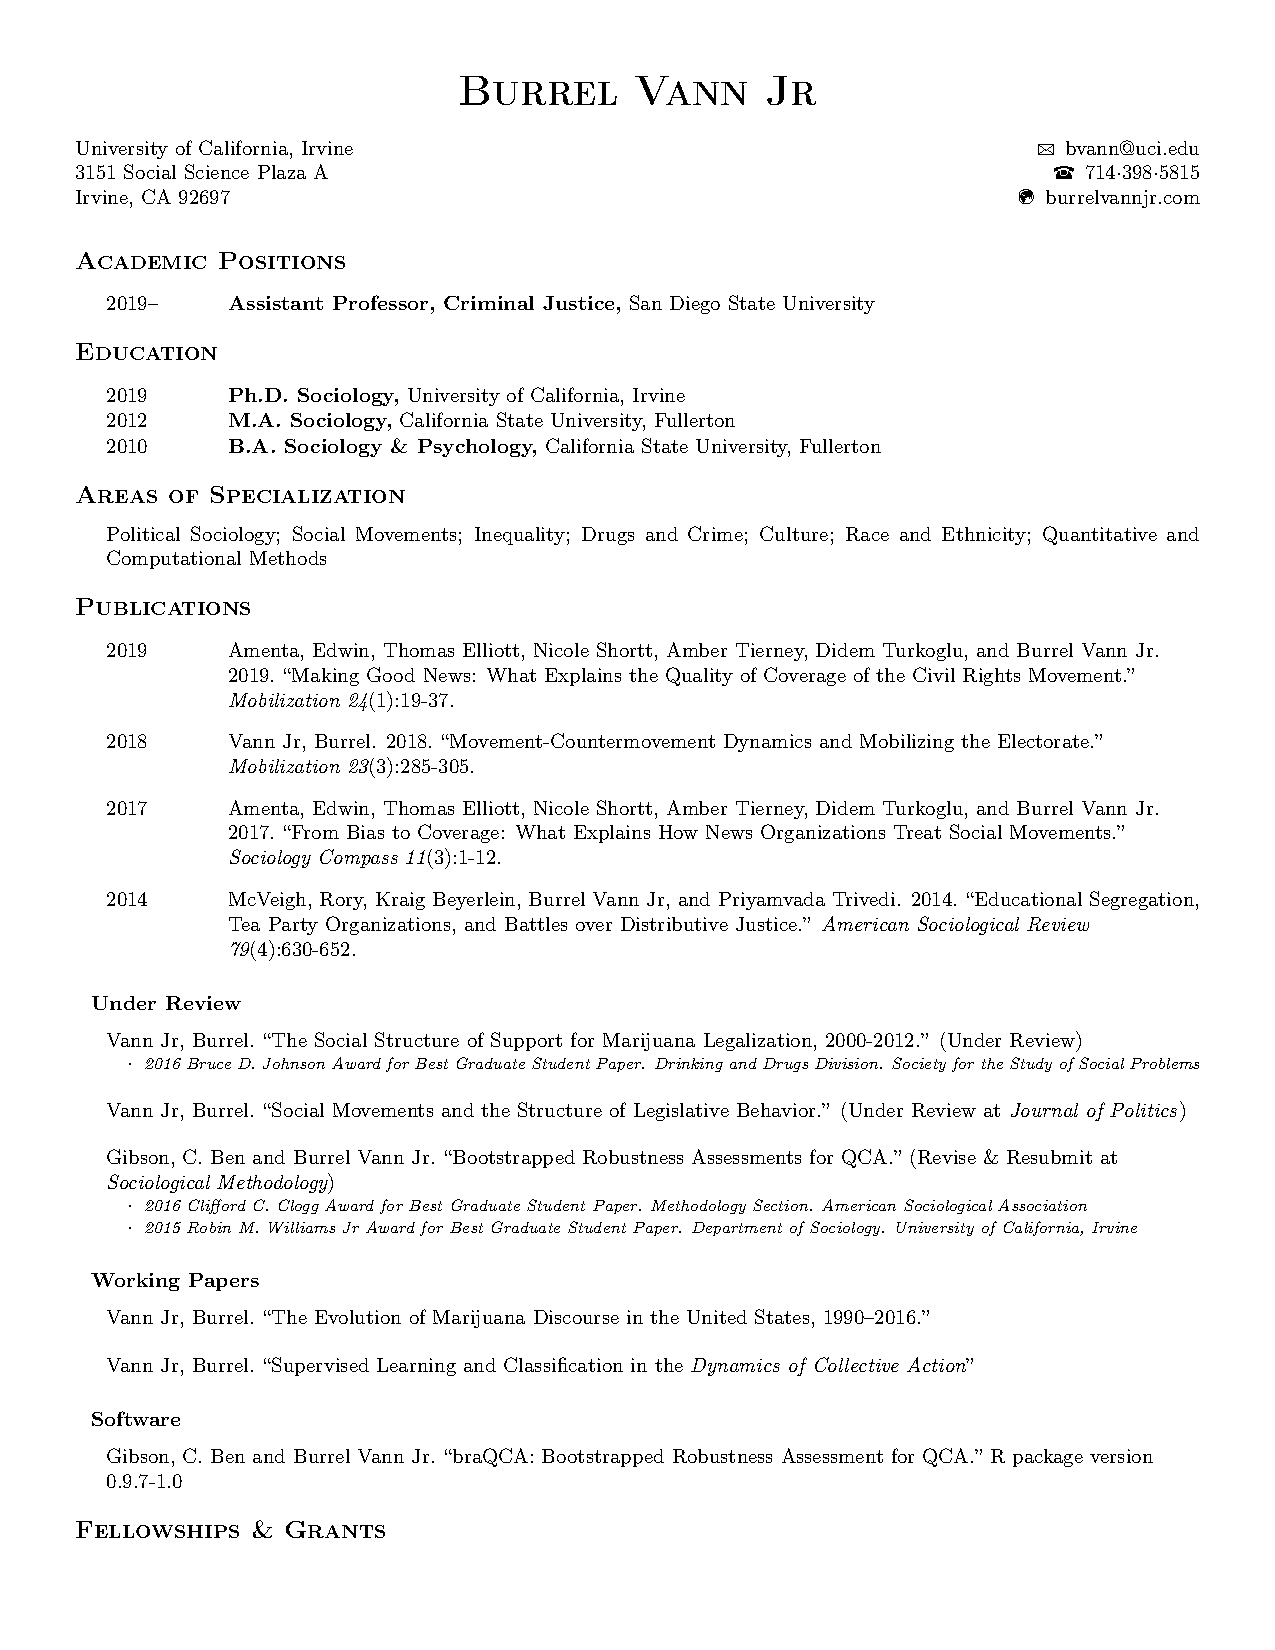
\includepdf{cv.pdf}
%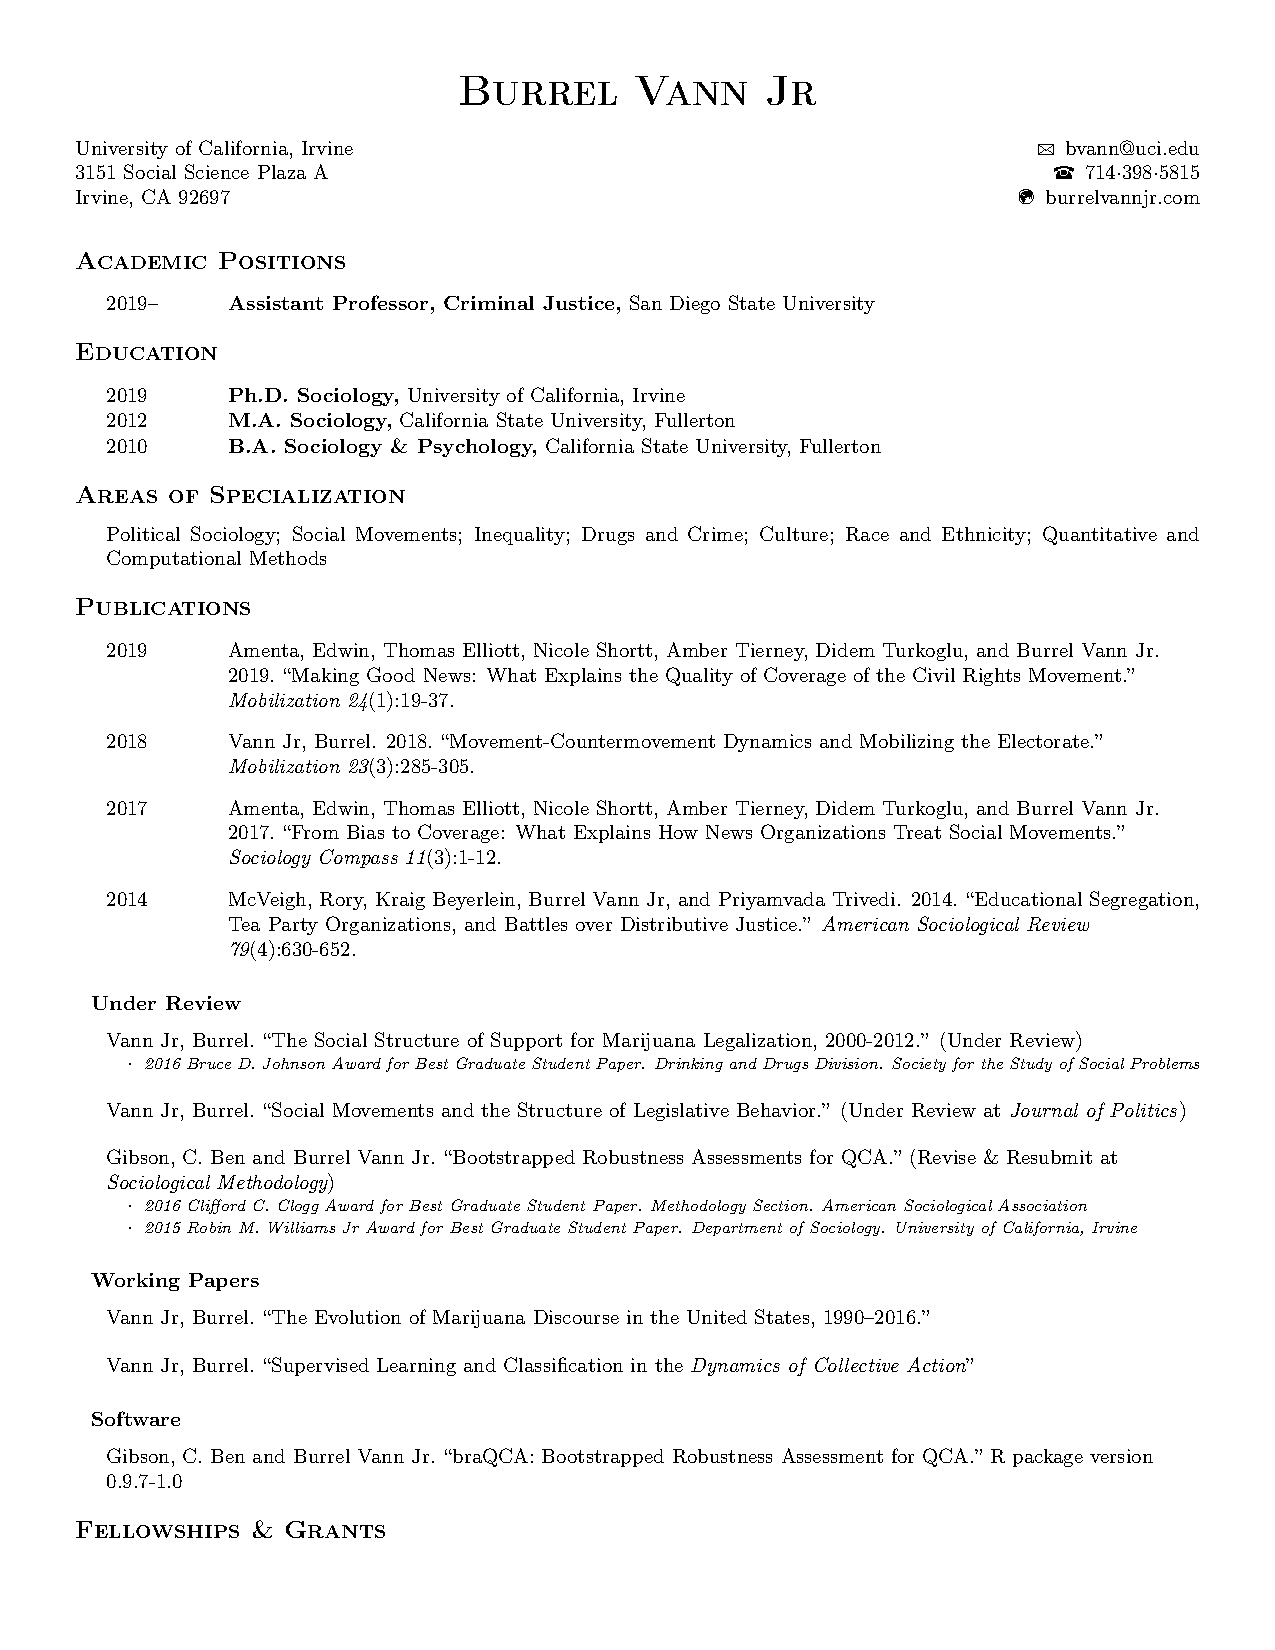
\includepdf[pages=1]{cv.pdf} 
%\IfFileExists{cv.pdf}{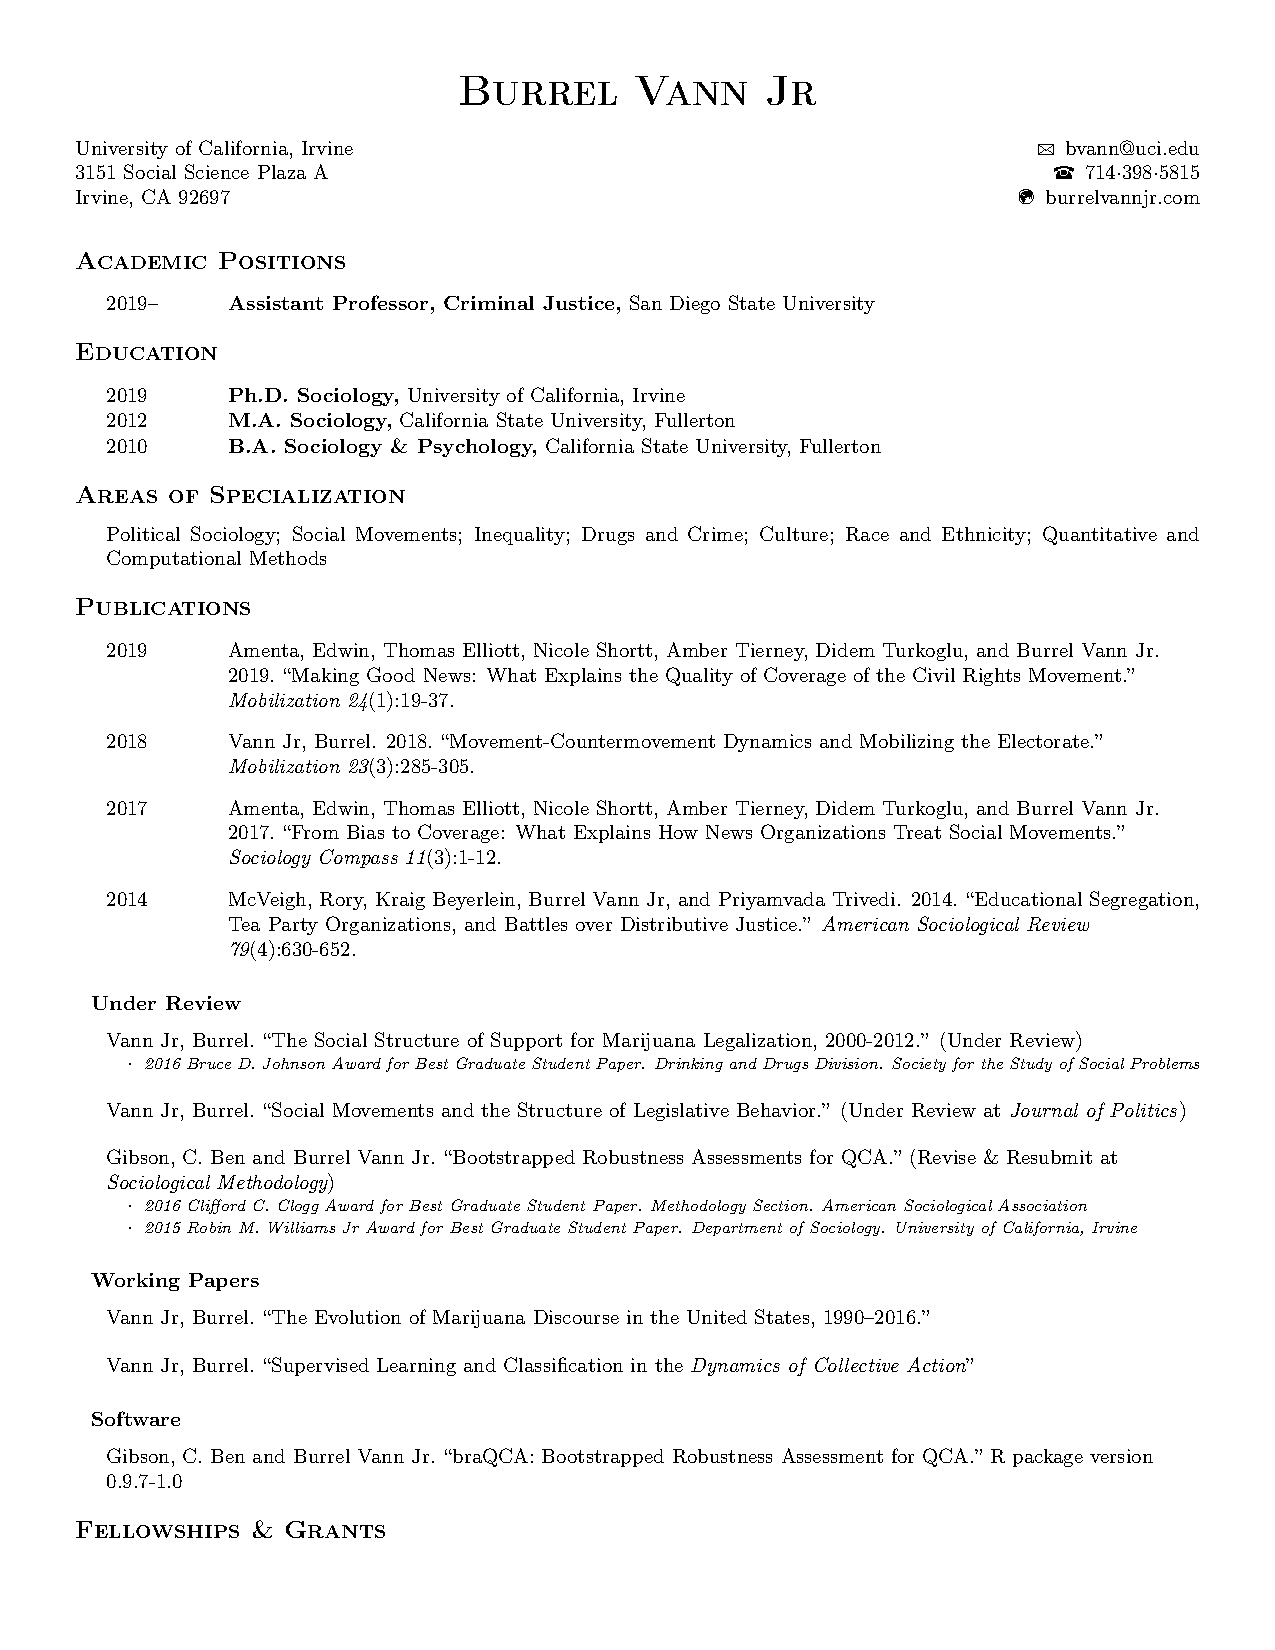
\includepdf{cv.pdf}}
%


%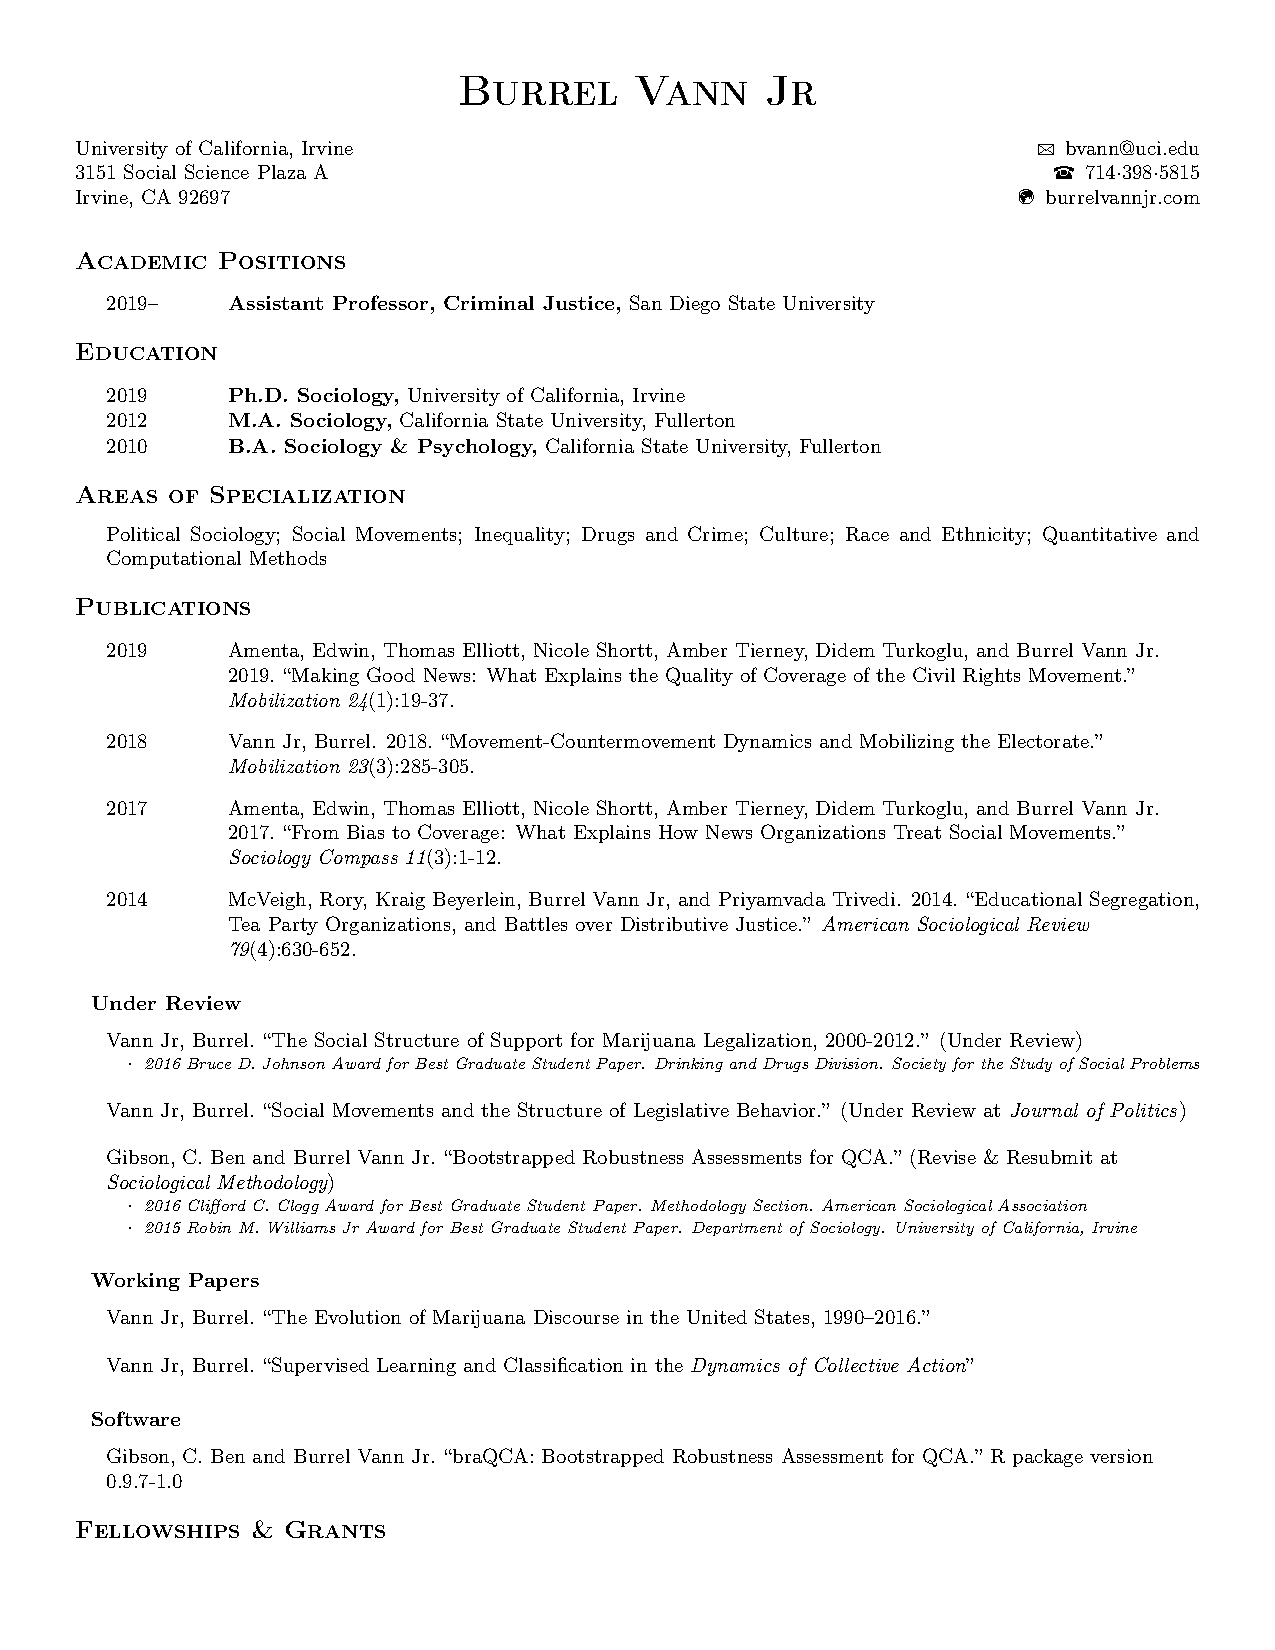
\includepdf[pages=1-]{cv.pdf}

% The abstract was previously limited to a maximum of 350 words, 
% but the UCI manual at https://etd.lib.uci.edu/electronic/td2e#2.2.1.
% currently does not indicate that there is any word limit for the abstract
\thesisabstract
{
  The abstract of your contribution goes here.
}


%%% Local Variables: ***
%%% mode: latex ***
%%% TeX-master: "thesis.tex" ***
%%% End: ***


% Add PDF document info fields
\hypersetup{
	pdftitle={\Thesistitle},
	pdfauthor={\Authorname},
	pdfsubject={\Degreefield},
}

% Uncomment the following to have numbered subsubsections (by default
% numbering goes only to subsections).
%\setcounter{secnumdepth}{4}


% Set this to only select a subset of the includes directives below.
% Very handy to speed up compilation if you're working on a certain
% part of your thesis. It conserves page numbers, references, etc.
% even for non-included files.
%\includeonly{chapter1}

%\usepackage{pdfpages} 

\begin{document}

% Preliminary pages are always loaded (TOC, CV, etc.)
\preliminarypages



% Include the different components of your thesis, in separate files.
% Using \include allows you to set \includeonly above.

\chapter{Introduction}
\begin{quotation}
\begin{singlespace}
\noindent {\footnotesize The sex fiend is a progressive criminal. He often begins with annoyances. He progresses to the sending of obscene letters, or exhibitionism. One finds him ``annoying'' children, or following women. For all these things, he often is merely fined, or given ``orders to leave town,'' or punished by a short jail sentences -- none of which deters him in the slightest degree from other and more serious offenses. And every sex criminal is a potential murderer.\newline

%\noindent Therefore, it would seem that the problem of the sex criminal is being mishandled... \newline

\noindent It should be determined, for instance, to what extent the recently widespread use of marijuana, or American hashish, has been responsible for the sex crime. \newline

\noindent Thus, a tremendous force may now be exerted toward the eradication of a drug which violently affects sex impulses.}\footnote{Hoover, J Edgar. September 26, 1937. ``WAR ON THE SEX CRIMINAL!'' \textit{Los Angeles Times}.}
\end{singlespace}
\end{quotation}
The above quote, appearing in the \textit{Los Angeles Times} in the fall of 1937, marked the beginning of the political fight, led by Harry J. Ansligner, to eradicate marijuana from America. Journalistic accounts like these, and the subsequent slew of restrictions on drugs, resulted in marijuana being conflated with fear, and ultimately prohibited in the United States through the Marihuana Tax Act of 1937. Terms like criminal, immoral, and deviant were often used, and it was assumed that marijuana was a danger to society. While early discussions of marijuana were usually negative, it took over half a century for the tone of coverage to shift towards attacking these perceptions:
\begin{quotation}
\begin{singlespace}
\noindent {\footnotesize In 1998, President Bill Clinton signed a provision that made people temporarily or permanently ineligible for federal financial aid depending on how many times they had been arrested and convicted of a drug offense... the effect was real and devastating: the people most in need of financial aid were also being the most targeted for marijuana arrests and were therefore the most at risk of being frozen out of higher education. \newline

\noindent Why would Democrats support a program that has such a deleterious effect on their most loyal constituencies? The fact that they are ruining the lives of hundreds of thousands of black and Hispanic men... barely seems to register. \newline

\noindent This is outrageous and immoral and the Democrat's complicity is unconscionable...

\noindent No one knows all the repercussions of legalizing marijuana, but it is clear that criminalizing it has made it a life-ruining racial weapon. When will politicians have the courage to stand up, acknowledge this fact and stop allowing young minority men to be collateral damage?}\footnote{Blow, Charles M. October 23, 2010. ``Smoke and Horrors'' \textit{New York Times}.}
\end{singlespace}
\end{quotation}

%Some of the most consequential legislation in this state's history has been enacted this way: most famously, Proposition 13, which put a cap on property tax increases and required a two-thirds vote by the Legislature to raise taxes.

%For anyone with money and political savvy, the ballot initiative has been an effective way to work around a balky Legislature. And the only way to change or repeal an initiative is to go back to voters.

%"Why try to pass something in the Legislature when you have the money to get something on the ballot and make it that much more difficult to change it later," said Joe Mathews, a longtime critic of the California governance system. "This serves people who have the money and have the power."

By the end of the twentieth century, newspapers began to change their tune. Editorials encouraging the passage of marijuana legalization were more frequent. Coverage began to be associated with medicine, social justice, and civil rights. Although marijuana remained illegal at the federal level, there was an uptick in state level activity to change marijuana laws statewide -- and the use of the ballot initiative proved relevant for enacting medicalization and legalization. Most noticeably, medical marijuana initiatives took off in the 1990s and 2000s and were successful in California's 1996 Proposition 215.

At the same time, there were changes in public opinion on marijuana -- by 2013, American public support for marijuana surpassed 50 percent \citep{gallup_2013}. This presents my puzzle: What accounts for the change in marijuana policies in the United States since 1990? 

Understanding marijuana policy change is important for substantive discussions about progressive policy change and the set of cases to which it belongs. Marijuana legalization bears some similarity to contentious and morality-related policies such as abortion rights, anti-prohibition, and lotteries \citep{gusfield_1963,andrews_and_seguin_2015,pierce_and_miller_1999,berry_and_berry_1990}. Marijuana legalization is similar to anti-prohibition and lotteries in that their perceived negative consequences and costs will only be incurred by those who make use of the policy \citep{mikesell_and_zorn_1986,berry_and_berry_1990}. Marijuana legalization differs, however, from anti-prohibition given alcohol's longstanding social and economic impact on American society \citep{andrews_and_seguin_2015}. Marijuana legalization also bears similarity to taxation policy \citep{amenta_and_halfmann_2000} in its generation of economic benefits. Finally, marijuana legalization has followed the reverse trend of tobacco policy. Tobacco use is tied to social and economic fabric of the United States. Yet, in recent years, has experienced some retrenchment --  due to increasingly negative connotations and beliefs attached to smoking. Marijuana, on the other hand, has become increasingly associated with medicinal and economic benefits. 

Legalization as progressive policy presents an intriguing case not wholly identical to others, yet one that can inform our understanding of the factors that contribute to progressive policy change. Moreover, given the recency of legalization, studying this policy can provide insight into the process of early adoption of policy in the long history of policy change. 

%This question is important because, as Ferree, Gamson, Gerhards, and Rucht (2002) observe, the media arena is the primary site for contests over meaning. How homosexuality is portrayed in the news media will have a powerful impact on on the larger public discussion of homosexuality. The news media is the main source of frame packages around an issue that get deployed in public conversations and when formulating public opinion (Gamson and Modigliani, 1989). Studying newspaper coverage of homosexuality can serve as a proxy for the larger public discussion over time, giving insight into how the general public understood homosexuality and how this changed over time. Additionally, changing the media portrayal of homosexuality is likely to lead to changes in the public discussion of homosexuality, so understanding how activists can change media portrayals of issues would contribute to understanding how movement can impact culture. 

%Social movements are an important part of the political landscape. They are vehicles by which people express grievances and work towards change. They have the potential to change both the political and cultural landscape. How they do this is still not well understood. Assessing how movements impact policy making and other political outcomes is complicated, making consensus on the mechanisms of influence elusive (Amenta and Caren, 2004). Even less well understood is how movements might have cultural impact. 

This project aims to fill some of these gaps by explaining how and why changes in the cultural, political, and structural landscape have contributed to changes marijuana policy in since 1990.


\section{Explanations for Policy Change}

What are possible explanations for changes in marijuana policy? I explore five perspectives to explain the legalization of marijuana. These five perspectives guide my analysis throughout this dissertation. In the conclusion, I evaluate how well each perspective helped in explaining my puzzle.


%\subsection{Public Opinion}

%Scholars have long studied the relationship between public opinion and policy change \citep{burstein_and_linton_2002}. The evidence suggests that the relationship is recursive. 

%Public opinion shifts when previously unused frames enter the media. These frames are in turn used in public discussions and are incorporated into personal formulations of opinion on an issue. Brewer (2003) explores how political knowledge mediates the impact of media frames on public opinion, and finds that undisputed media frames are more likely to influence public opinion than disputed frames.



\subsection{Political Institutional Contexts}

One possible explanation for the shifts in marijuana policy is related to political institutional contexts. Certain contexts provide more opportunities for policy change than others. Political context theories often focus on the role of elite allies in government that may contribute to the overall success of a policy change \citep{amenta_et_al_1994,amenta_2006}. Research in political sociology and political science has focused on the role of left- or reform-oriented parties in the passage or adoption of progressive policies \citep{amenta_and_elliott_2019,amenta_et_al_2005,korpi_1983}. Moreover, whether or not elite allies hold majorities in government is important for the likelihood for policy change\citep{ansolabehere_and_snyder2006,winters_1976,abramowitz_1983,campagna_and_grofman_1990}. And because political officials as allies want to make good on their promises, they will often support or sponsor policies that accord with the interests of their constituents \citep{page_and_shapiro_1983,mayhew_1974,downs_1957,stimson_et_al_1995}. 

Voting results are also an important part of the political institutional environment. Support for specific parties signal to both constituents and political officials that certain types of policy change are possible or not \citep{amenta_and_elliott_2019}. These characteristics pique the interests of politicians and constituents to support specific policy changes \citep{berry_and_berry_1990,boushey_2016}. 

Public opinion is also an important part of the political institutional environment \citep{burstein_1998,burstein_2003}. Similarly, public opinion serves as a signal about what sorts of policies are possible. Therefore, public opinion reveals the saliency of political issues for constituents as well as political officials \citep{pacheco_2012,nicholson-crotty_2009}.



%What exactly counts as political opportunity is not well defined (Goodwin, Jasper, and Khattra, 1999). It has been used broadly to include virtually all macro-level effects on movement mobilization and outcomes. In an international comparative context, political opportunity refers to the openness or closedness of a political system (Kriesi, 2006). In the single nation context, political opportunity refers to the configuration of allies, antagonists and bystanders. Scholars have tended to interpret this as how friendly political institutions are at any given time, as well as whether public opinion is on the movement's side. 

%The political opportunities that lead to mobilization and policy success may also lead to increased and better media coverage of movements. Just as political opportunities can signal to movements that the time is right for mobilization, political opportunities could send signals to media professionals to pay more attention to an issue, or to treat an issue differently. These signals could include the election or appointment of new politicians, or the passage of new reforms regarding an issue. Political opportunities also influence movement's tactics in the media arena (Rohlinger, 2006), which could, in turn, influence the coverage of the movement's issue. Previous research has found mixed results for political opportunity?s influence of news coverage of movement organizations, as it seems to influence coverage in partisan news outlets, but not in mainstream outlets (Amenta, Caren, and Stobaugh, 2012; Rohlinger, Kail, Taylor, and Conn, 2012).


\subsection{Policy Feedback}


An alternative explanation related to the political context involves the legacy of policy reforms or policy feedback around an issue. Drawing on ideas of increasing returns \citep{pierson_1996,pierson_2000}, policy reforms will have both immediate, as well as long lasting benefits for future policy change \citep{amenta_et_al_2012}. Policies often lead to institutionalized benefits to a specific group of people. These benefits can provide a boost in the efficacy of future advocacy on the part of beneficiaries \citep{amenta_and_caren_2004}. 


%If the group is represented by a movement, organizations affiliated with this movement can gain an additional benefit in the form of acceptance (Amenta and Caren, 2004). Policy reforms may cast organizations that represent the constituencies benefiting from the reforms in a more legitimate light. This could lead to the organizations having access to more and better resources, enabling them to be more effective in future advocacy. Furthermore, this increased legitimacy can lead to members of the movement being placed in positions of authority within the state. %As an example, AIDS activists were appointed to a Presidential task force on AIDS in the 1990s (Epstein, 2007). These members were then able to more directly influence policy on their issues, further improving its policy profile. 


%Applying this to the media arena, the political process is typically a highly newsworthy process, most newspapers assign one or more beats to covering politics. Movements and their actors are likely to be covered if a policy they are advocating for is making its way through the political process. If the policy is successful, the movement may be seen as more legitimate not only by state actors, but also the media, leading to further coverage, especially as the policy is implemented. This effect will be cumulative, with more policy successes leading to more legitimacy in the media arena. Additionally, if a movement actor is appointed to a state position, they will receive the benefit all state actors receive in the media arena, with much easier access and more frequent coverage by the media (Gans, 1979; Oliver and Maney, 2000; Sobieraj, 2010; Tuchman, 1978).


%\subsection{Crisis}


%Another possible explanation for the change in coverage of homosexuality concerns crises (Snow, Cress, Downey, and Jones, 1998). Crises are typically highly newsworthy, having several characteristics journalists look for in deciding what's news (Gans, 1979). Crises are unusual, outside of the routine of daily life. Crises typically impact a large number of people. Crises also usually involve the government trying to solve the crisis. Newspapers are likely, then, to devote a fair amount of coverage to crises. Movements may be able to benefit from this coverage if they are affiliated with an issue impacted by the crisis, and crises can spawn entirely new movements as those affected mobilize themselves (Snow et al., 1998). 

%The partial meltdown at the nuclear reactor at Three Mile Island is an example of this type of crisis. Local pre-existing anti-nuclear organizations experienced a tremendous surge in members after the accident, and new organizations were founded in communities closest to Three Mile Island to oppose the restart of the Unit 1 reactor and impose strict regulations on the cleanup of Unit 2 (Cable, Walsh, and Warland, 1988). The Three Mile Island accident also introduced new framing packages that significantly shifted public opinion against nuclear power (Gamson and Modigliani, 1989). 

%Crises may also undermine the authority of the status quo, bringing attention to deficiencies of the dominant groups (Bail, 2012). Especially if the government is seen as contributing to the disaster, or negligent in addressing the disaster, official authorities may lose legitimacy on the issue (Snow et al., 1998). The news may turn to movements in these cases in the search for new experts. Movements could potentially be considered alternative experts on the issue, or they may be used as ``authentic'' responses to the crisis Sobieraj (2010). Either way, movements can expect to receive increased coverage in the wake of a crisis that involves an issue they are mobilized around. This coverage offers movements the opportunity to inject new ways to think about the issue, and the crisis may have destabilized the dominant discourse in ways that make the movement especially influential in this area.


\subsection{Cultural Context/Discourse}

Mass media are central for making sense of relevant events \citep{gamson_and_modigliani_1989}. According to \citet{ferree_et_al_2002} are a master forum within which actors compete for coverage of their issues \citep{amenta_et_al_2012}, which serves to identify and redefine, which can shape public perceptions of issues. Importantly, news organizations operate by a set of ``news values'' procedures that helps to identify what \textit{counts} as news \citep{amenta_et_al_2012,galtung_and_ruge_1965}, which not only affects the selection of topics to be covered \citep{galtung_and_ruge_1965} but also the ways in which these topics are covered.

The news values process necessarily selects on official or institutional news coverage \citep{schudson_2002,gitlin_1980,gans_1979} that tends to center on institutional political action and actors, because they are seen as newsworthy \citep{amenta_et_al_2012}. Relatedly, the economics of news media puts various pressures on the news to run stories that are not too gruesome, not too critical, and not too controversial. 

These and similar pressures lead to stories that do not venture too far from mainstream ideas and beliefs, so media coverage of an issue is likely to be close to public opinion about that issue \citep{gamson_and_modigliani_1989}. News can also influence public opinion. For example, \citep{gamson_and_modigliani_1989} find that the appearance of new frames around nuclear energy in news coverage influenced public discussion of the nuclear energy issues, which ultimately shapes public opinion about the issue.

Yet, organizations and other actors in the environment also have the ability to shape these frames. Recent research on the cultural consequences of social movements \citep{earl_2004} finds that organizations can impact public conversation about issues \citep{bail_et_al_2017} and initiate discursive change by offering their own diagnoses of and solutions to problems \citep{bail_2012,snow_et_al_2007,benford_and_snow_2000}. By injecting new frames into the broader discursive environment, organizations can shape the evolution of discourse. Although frames that `fit' the broader discursive environment \citep{mccammon_et_al_2007} or those that articulate widespread beliefs usually win out \citep{mccammon_et_al_2001,snow_et_al_2007,gamson_and_modigliani_1989}, alternative or fringe frames have the ability to alter discourse on a topic \citep{bail_2012}.

These studies suggest, then, that news media is not likely to (but can) feature media frames that are from the fringe of public discourse, but the media frames they do feature have an impact on public opinion or support for an issue. 

\subsection{Advocacy Organizations}

Perhaps marijuana advocacy organizations influenced marijuana policy change by way of being covered about the marijuana issue. Scholarly attention has traditionally focused on how the news media covers advocacy organizations \citep{amenta_et_al_2009,andrews_and_caren_2010}. Understanding this process is an important first step, as gaining coverage may be necessary to influence the public discussion of an issue. Coverage gives organizations an opportunity to inject new framing packages into the media arena, potentially changing the conversation around an issue \citep{gamson_and_modigliani_1989}. Although research on social movements typically focuses on the impact of protest on coverage \citep{earl_et_al_2004,oliver_and_myers_1999}, marijuana advocacy organizations rarely engaged in the type of protest necessary to gain coverage. Coverage of organizations may provide better opportunities for influence the discussion of an issue. 


\subsection{Structural Contexts}

Perceptions of and support for political issues results from the contexts within which people are embedded \citep{blau_1977a,blau_1977b,mcveigh_and_diaz_2009}. Importantly, the distribution of people and their interests across space can shape aggregate support for progressive policy change. \citet{mcveigh_et_al_2014a}, for example, find that the distribution of the highly educated had implications for support for conservative mobilization. Structural contexts consists of the presence or absence of certain attributes \citep{blau_1977a,blau_1977b,blau_and_duncan_1967}, as well as their spatial spread across a local environment. The impact of social structure on policy change can also involve the presence or absence of advocacy organizations \citep{vann_jr_2018,soule_and_olzak_2004}, aspects of the lived environment \citep{olzak_and_soule_2009} as well as levels of segregation within local contexts \citep{andrews_and_seguin_2015,olzak_et_al_1994}. 







While any one of the previous perspectives may provide a better explanation for the changes in the passage of marijuana legalization than other perspectives, they do no operate in a vacuum. Each of the processes described by the perspectives are likely to influence and be influenced by the processes of other perspectives. For example, amenable political contexts may lead to additional coverage of marijuana, but the nature of this coverage is likely to be influenced by policy reform mechanisms. My analyses take into account these processes.


\section{Data}


To explain my puzzle, I collected a variety of data. Importantly, my dependent variables include data on marijuana initiative voting and on newspaper coverage of marijuana from 1990 to 2016. The battle for marijuana legalization only recently shifted to state governments. Therefore, I rely on voting data from ballot initiatives\footnote{rather than state legislative hearing date because these hearings were few and far between} and newspaper articles about marijuana. From 1990 to 2016, states with the provision of the ballot initiative became sites of policy change on the marijuana issue. Thus, I use data from citizen/voter initiatives as measures of support for legalization. These data come from the Secretary of State websites for each state. 

%%%%%%%%%
%%%%USE THIS
%I searched the ProQuest archives for mentions of ``marijuana.''  This resulted in 5,893 articles across 100 newspapers. I chose these sources because they are widely circulated, represent both geographic diversity, and can be mapped onto to counties and states, which allows me to geolocate discourse about marijuana over time. I also searched the ProQuest newspaper archives for mentions of one of the four major marijuana advocacy organizations. In order to be included, the organization should be politically oriented with the goal of progressive marijuana policy change (e.g. decriminalization, medicalization, and legalization of marijuana), which excludes organizations like the NAACP, which does not primarily engage in marijuana advocacy. Using a list of search terms generated for each organization, I identified 787 articles, across 62 newspapers, mentioning at least one of these organizations. 










%To collect data on the content of the coverage, I created a 0.5% sample per year from the coverage of homosexuality, with a minimum of five articles included in each year. I supplemented this with a 2% sample of the coverage of LGBT and AIDS organizations. This resulted in 720 articles to code. I coded information about the article including the author, the occasion for coverage, and the type of article. I coded information about any social movement organization mentioned in the article, both LGBT and AIDS, and nonLGBT organizations. I also coded every paragraph that mentioned homosexuality in some way, including information on the speaker, the valence of the paragraph, and what terms and claims appeared. I discuss these measures in more detail where relevant in the following chapters. 


\section{Summary of Dissertation}


The rest of the dissertation is laid out in the following way. In chapter 2, I explore the amount and type of coverage newspapers gave to marijuana, from 1990 to 2016. I do so by considering the various frames associated with marijuana. Specifically, I separate the analysis into coverage of marijuana alone and coverage that also included marijuana advocacy organizations. I find that during the early years, marijuana coverage was mostly negative, and centered on a variety of frames. In later years, coverage became less negative (more neutral and positive) and frames shifted towards discussions of politics and revenue creation associated with marijuana legalization. This suggests that when controversial political issues enter public discourse by being put on the political agenda, a number of frames will be juxtaposed with one another and compete for dominance. But, given the controversial nature of these issues, as coverage of these issues matures, to maintain coverage, they must be linked to or framed as non-controversial, ``traditionalist,'' or quotidian \citep{snow_et_al_1998} behavior. 


Next, in chapter 3 I analyze the rate of adoption of legalization. I use event history analysis to investigate what explains the rate of adoption of legalization across the American states, from 1990 to 2016. I find that positive coverage on marijuana increases the rate of passage, particularly in states with the ballot initiative. I also find that Democratic support and political competition increase the rate of legalization. Moreover, prior histories with marijuana in a state, by way of medicalization, increases the rate at which states adopt legalization over time. 

Chapter 4 takes a structural approach to understanding legalization. Using ordinary least squares analysis of county-level support for legalization initiatives between 2000 and 2016, I examine how local level factors that contribute to increased voter support for policy change. I find that parental segregation and (the absence of) inequality ultimately create contexts within which marijuana legalization is viewed as non-threatening to the community. 

Finally, Chapter 5 concludes the project, summarizing how each perspective contributed to my explanation of the outcomes investigated in chapters 2--4. I argue that discourse about marijuana became less negative as a result of framing shifts. This shift in framing ultimately helped to speed up the process of legalization across the U.S. Yet, at the local level, segregation and inequality play a role in aggregate support for legalization. I discuss limitations of this project, as well as directions for future study.



%%% Local Variables: ***
%%% mode: latex ***
%%% TeX-master: "thesis.tex" ***
%%% End: ***


\chapter{The Discursive Shift on Marijuana Legalization}



%\begin{abstract}
%\begin{singlespace}
%What drives discourse about drugs? This study examines the dramatic decrease in negative coverage about marijuana in U.S. states from 1990 to 2016. I argue that, when focusing on liberties/freedoms, patients, and linking marijuana legalization with voting, the dominant discourse on contested issues can shift away. Results from logistic regression analyses in newspaper articles demonstrate that the shift away from negative discourse on marijuana was significantly influenced by shifting the discussion towards these topics. 
%\end{singlespace}
%\end{abstract}
%\newpage

\bibpunct[:]{(}{)}{;}{a}{}{,} % new punctuation for these, replace parentheses before and after citealt, and replace citealt with citep



%--------------------------------------------------------------------------------------------------------------------------------------
\section{Introduction}


Examination of frames, narratives, and discourse has been central to sociological understanding of cultural and political change \citep{ghaziani_and_baldassarri_2011,vasi_et_al_2015,bail_2012,mccammon_et_al_2007}. I contribute to this line of inquiry by investigating whether and how framing about marijuana changed over time. Coverage of marijuana presents an ideal case with which to examine discursive shifts, given that the ways in which marijuana was covered has moved away from negative discussions that centered on crime and danger \citep{newhart_and_dolphin_2018,bonnie_and_whitebread_1970,rosenthal_and_kubby_1996}, towards positive and neutral discussions regarding the benefits of marijuana and marijuana legalization \citep{mosher_and_akins_2019}. To what extent has there been a general shift away from negative coverage of marijuana? And to what extent have new frames come to dominate the discussion of marijuana? 


%I advance this body of work by examining the outcome of discursive shifts about marijuana. Given that, until recently, many politicians did not want to tackle the marijuana issue for fear of appearing less-than-tough on crime \citep{rosenthal_and_kubby_1996}, shaping media discourse about marijuana proved critical for advancing legislation on marijuana. Why did coverage of marijuana change, or become less negative, over time? Most importantly, to what extent did the narratives about marijuana contribute to this shift?

%I argue that discursive change is initiated by a variety of mechanisms, and that discourse changes by altering the conversation attached to an issue. Reframing of an issue in new and  culturally relevant ways \citep{gamson_and_modigliani_1989} that provide alternative understandings to longstanding debates \citep{bail_2012,snow_2004} can shift public perceptions and dominant discourse on an issue over time \citep{ghaziani_and_baldassarri_2011,baldassarri_and_bearman_2007}.

With recent advances in the field of computational social science, it has become easier than ever to gather, code, and analyze large corpuses of text for the purpose of tracking discursive trends \citep{bateman_et_al_2019,bail_2012,vasi_et_al_2015}. As such, I rely on webscraping techniques to gather newspaper articles about marijuana over time, breaking these articles as either covering marijuana with or without coverage of a marijuana advocacy organization. I, next, rely on automated text analysis to code the valence of each news article. Finally, using a combination of inductive and deductive approaches, I create a list of eight possible frames (and keywords associated with these frames) that may have appeared in marijuana coverage. I use automated coding to categorize each article has having the presence or absence of each frame. 


In this article, I shed light on the ways in which frames about marijuana changed in the United States between 1990 (when marijuana initiatives began to take off) and 2016. I demonstrate various characteristics about marijuana coverage and discourse over time. First, I show that, after 1996, when marijuana medicalization was on the ballot in California, coverage of marijuana increased dramatically. Secondly, I show that coverage of marijuana became decreasingly negative and increasingly neutral over time. Thirdly, I show that frames centering on revenue creation and politics came to dominate the discussion of marijuana, followed by framings related to rights and patients. 


% various framings or narratives about contested issues impact overall discourse. I do so by examining the impact narratives about marijuana on general media coverage of marijuana in the U.S. from 1990 to 2016. In particular, I examine whether the shift towards less negative discourse about marijuana resulted from various framings about marijuana. 


%American public opinion on marijuana legalization has undergone rapid change over the past two decades (Gallup 2013; Pew Research Center 2013). In 2006, a Colorado ballot initiative that would have legalized marijuana was handedly defeated; fewer than one quarter of Colorado counties supported the initiative. The issue was revisited in 2012, and with 55 percent of the vote, ushered in a new era of marijuana reform in the United States. The rapid growth in support for legalization set off a wave of state-level activity (as shown in Table 1), as organizations, voters, and politicians attempted to reform marijuana policy. Despite growing support for legalization, opponents generally perceive legalization as harmful to society; supporters, on the other hand, view legalization as an opportunity to remedy social problems (Caulkins et al. 2012; Rosenthal and Kubby 1996). Supporters of legalization argue that regulation and taxation of marijuana would help reduce crime, addiction, and drug abuse while also providing necessary revenue for educational and rehabilitative programs. 

%Perceptions of opportunity are the product of social construction processes, developed through social interaction, and are dependent upon the contexts in which people are embedded. In this article, I examine how residential segregation in local contexts that is based on the presence of households with (or without) children ? what I term, parental segregation ? influences voting behavior in support of policy change. This investigation is rooted in my understanding of how segregation has implications for how opportunity is perceived and acted on. Class-, race-, and education-based segregation operate by concentrating opportunities for some portion of the population while restricting access for others. Class segregation, for example, can restrict poor residents? access to quality education and employment (Massey and Denton 1993; Wilson 1987). Moreover, segregation concentrates individuals who have the knowledge and resources necessary to recognize and act on those opportunities. Importantly, segregation can facilitate reactive political action when it is vulnerable to penetration, or threatened by the increasing presence or political power of minority groups (McVeigh et al. 2014; Beisel 1997, 1990; Andrews and Seguin 2015). Limited contact with minority groups can lead majority group members to view racial minorities and the poor as responsible for their disadvantaged condition (Beisel 1990, 1997; Higham 1955). However, these beliefs may not resonate where actual threats do not exist. In fact, segregation concentrates residents of similar groups and decreases intergroup exposure, which can mobilize progressive political action (Galbraith and Hale 2008).

%The recent rise in ballot initiatives devoted to marijuana legalization provides a unique opportunity to examine how structural features of local contexts shape political behavior related to opportunity. The fight over marijuana?s legality is important in its own right because it involves battles over meanings of civil liberty, drugs, medicine, abuse, and morality. The growth in support for legalization is in part driven by backlash against prohibition and claims that legalization could contribute to safer communities by helping to shrink the size and influence of the illegal drug market (Marijuana Policy Project 2015; Rosenthal and Kubby 1996; Caulkins et al. 2012; Blocker 1989). While opposition exists, it remains highest amongst groups arguing that legalization would negatively impact communities, families, and children ? namely parents.

%In this article, I aim to shed additional light on marijuana legalization in the United States. I do so by considering whether the residential segregation of households with children from households without children (or, put another way, parents from nonparents) may facilitate support for policy change, such as marijuana legalization, that provides an opportunity to remedy social ills. Moreover, because perceptions of opportunity resulting from potential policy change is reflected in structural relations, changes in local communities may have a diminishing effect on support for marijuana reform. As such, I expect the effects segregation to be strong in unchanging communities.




%--------------------------------------------------------------------------------------------------------------------------------------
\section{Discursive Change Processes}

Discourse has been the subject of recent academic work, with most focusing on the role of social movements or advocacy organizations in initiating discursive change \citep{bail_2012,earl_2004,mccammon_et_al_2007,ghaziani_and_baldassarri_2011,vasi_et_al_2015,gamson_and_modigliani_1989}. In particular, organizations offer their own diagnoses of and solutions to problems and can impact public discourse on an issue injecting novel, highly resonant frames into public discussion \citep{benford_and_snow_2000}. Frames that `fit' the broader discursive environment \citep{mccammon_et_al_2007} or those that articulate widespread beliefs and values usually survive over alternative frames \citep{mccammon_et_al_2001,snow_et_al_2007,gamson_and_modigliani_1989}, because their frames ``are more easily integrated into broader media narratives'' on an issue because these frames seem more familiar \citep{bail_2012} and appear realistic or legitimate. 

Coverage of issues is critical to this process \citep{amenta_et_al_2009,ferree_et_al_2002}. Therefore, mass media are important to cultural change. Mass media are central for making sense of relevant events \citep{gamson_and_modigliani_1989}, and serve to identify and redefine issues for the public. These discussions can shape audience perceptions. While media are a master forum within which actors compete for coverage of their issues \citep{amenta_et_al_2012}, media organizations themselves operate by a set of procedures that can also have effects on discourse on issues. 


News organizations make decisions about what counts as ``news'' \citep{galtung_and_ruge_1965}. News is selected based on its timeliness/currency, the impact of the events to be covered, and the proximity of those events to potential readers (with local news angles being considered important, particularly in national stories). In particular, politics receives the most coverage because political decisions have high impact and include prominent people. In addition, reporters often have increased access to political actors. In sum, much of what counts as news revolves around institutional political activity, including stories about politicians, bills being discussed or laws being passed \citep{amenta_et_al_2012}. Therefore, it is reasonable to assume that discursive change on marijuana may have occurred by way of institutional political actors. However, as is the case for many hotly contested issues like marijuana, engaging in discussions on these topics provides little political advantage, rendering many political actors unwilling to even discuss the issue. In particular, when dominant discourse on a topic is negative, political actors will be unwilling to discuss the issues in new, more positive ways, for fear of reprisals from their constituents in the form of lost votes. 

Given the tendency of journalists and the norms of news-gathering organizations to seek out official sources \citep{schudson_2002,gitlin_1980,gans_1979}, especially during times of high attention to the issue in the news cycle \citep{baumgartner_and_jones_1993} the general lack of discussion by political actors creates opportunities for other actors (including journalists themselves) to, not only, provide alternative narratives on an issue, but shift the character of discourse by linking the issue with alternative topics. 

%that are different from dominant discourse on that topic can be a political disadvantage


I argue that, by linking discourse about contested issues to additional, more institutionalized topics or narratives, journalists can facilitate a stark transformation in public understandings on an issue, and call into question the legitimacy of dominant representations. Initial marijuana discourse centered on criminality and the negative educational, occupational, and mental effects of marijuana use. In recent years, however, this discourse has given way to increasingly positive (or fewer negative) discussions of marijuana's medical, community, and economic benefits. This coverage has shifted the arenas within which marijuana was discussed by linking marijuana with narrative topics related to medicine, rights, freedom, economics, crime, and policing. Yet it remains unclear whether and how these new narrative topics contributed to the discursive shift away from a dominant negative discourse about marijuana. 

%In addition, the movement has devoted much of it's resources not on protest as a means of changing public definitions of marijuana, but on local and statewide initiatives, gaining media coverage of their issue, and on holding local community-based meetings. 


%--------------------------------------------------------------------------------------------------------------------------------------
\section{Marijuana Discourse Across Time}


According to historians studying marijuana, initial depictions of marijuana were positive, centering on the medicinal and material benefits of cannabis \citep{bonnie_and_whitebread_1970,rosenthal_and_kubby_1996}. While there was relatively little coverage of marijuana during this time \citep{bonnie_and_whitebread_1970,mosher_and_akins_2019}, what little coverage did exist was positive. However, during the 1930s, the valence of this coverage shifted as a result of political and bureaucratic changes. 

In 1930, President Herbert Hoover established the Federal Bureau of Narcotics (FBN) and appointed Harry J. Anslinger as commissioner. According to scholars, Anslinger was in charge of repurposing prohibition funds, and, in noticing that Americans were enjoying Mexican and Native-American cannabis, Ansligner chose to direct his Bureau's resources toward cannabis \citep{newhart_and_dolphin_2018}. In fact, Anslinger used media to paint cannabis in a negative light as a way to ramp up public opposition to the substance. Anslinger used stories and advertisements in newspapers (including William Randolph Hearst's newspapers) to portray cannabis as dangerous to women, children, and society \citep{mosher_and_akins_2019}. Hearst, for his part, stood to lose economically if American cannabis use expanded -- he invested in wood pulp, which he used for his papers, and the expansion of hemp (which could also be used for cheaper newspaper manufacturing) put him in danger of losing his fortune. Through a campaign of ``yellow'' journalism, which enabled Anslinger to rebrand the drug with the more Native-sounding name marihuana (or marijuana) instead of cannabis, Anslinger and Hearst were able to associate the drug with a source or group of people responsible for the drug problem: immigrants, Mexicans, and indigenous ``others.'' Through newspapers, Anslinger and Hearst were able to ``sell'' marijuana as dangerous -- relying on a fear narrative that argued that only through cannabis prohibition could America's children, women, and society be protected \citep{mosher_and_akins_2019,newhart_and_dolphin_2018,rosenthal_and_kubby_1996}. 

Within a few years, these narratives took hold. In fact, over this time, marijuana became increasingly associated with criminality -- and in particular, minority criminality. During this time, marijuana was thought to be used mainly by minorities (freed Black slaves and Mexican immigrants) and had psychological properties that made them more prone to violence \citep{caulkins_et_al_2012,slaughter_1987}. These dominant narratives came to be used in arguments to Congress in favor of a full ban on marijuana -- resulting in the creation of the Marihuana Tax Act of 1937 \citep{newhart_and_dolphin_2018}. 



Between the 1930s and 1960s, the Act faced tough criticism in state and federal courts, as the judicial system worked to clarify the parameters of the law as well as what could and could not be enforced \citep{bonnie_and_whitebread_1970,mosher_and_akins_2019}. Around this time, advocacy organizations emerged to fight for access to marijuana \citep{newhart_and_dolphin_2018}. In 1970, the first marijuana movement organization, the National Organization for the Reform of Marijuana Laws, was created to fight against marijuana prohibition and to move public opinion on marijuana so as to enable full legalization of marijuana for all people. It wasn't until the mid-1990s and early 2000s (during NORML's fight for medicinal marijuana use on the California ballot) that other organizations such as the Marijuana Policy Project (1995), Students for Sensible Drug Policy (1998), and the Drug Policy Alliance (2000) joined the fight -- each with a specific purpose for legalization. For example, MPP would work on marijuana policy specifically while DPA would focus on both marijuana and similar narcotic policies, and SSDP would work to change the minds of youth, particularly on college campuses. 

According to prior research, marijuana discourse in the shifted in the 1960s. During this time, coverage of marijuana centered on the freedom to use the drug \citep{mosher_and_akin_2019}. 

In the mid-1990s, private individuals began to fight against marijuana prohibition in the United States by sponsoring marijuana medicalization initiatives in states with direct democratic processes. During this same time, journalists began to 1) give increasing attention to marijuana, and 2) link discussions of marijuana with additional topics. Some scholars have indicated that during this time, narratives about marijuana began to become more positive, as coverage tended to focus on the political aspects of initiatives or voters, the benefits to patients, and the rights of cannabis users \citep{newhart_and_dolphin_2018,mosher_and_akins_2019,bonnie_and_whitebread_1970}. Over time, the trajectory of marijuana legalization is such that states (under federal prohibition of marijuana, and those with the initiative/referendum process) would first propose medical legislation, followed by recreational legalization legislation. During this time, marijuana coverage began to link with larger ``American'' values of liberties and freedom, in addition to shifting to the benefits of legalization for revenue, creating resources for rehabilitation, decreasing crime, and altering policing practices -- especially in communities of color \citep{mosher_and_akins_2019,newhart_and_dolphin_2018}.

Given this shift, I expect that these various narratives should have distinct impact in the decrease in negative attention to marijuana. Below, I outline the ways in which I study these effects. 

%\subsection{\textit{The Shift: Reframing and Positive Discourse about Marijuana}}



%\input{/Users/burrelvannjr/Dropbox/Professional/Research/Projects/dissertation/chapters/ch2.movements-and-discourse/paper/figures/figure2.tex}

%\input{/Users/burrelvannjr/Dropbox/Professional/Research/Projects/dissertation/chapters/ch2.movements-and-discourse/paper/figures/figure3.tex}


%--------------------------------------------------------------------------------------------------------------------------------------
\section{Data \& Method}

Given my interest in \textit{whether} and \textit{how} marijuana discourse shifted over time, I analyze text from print news media across the United States. To do so, I rely on the ProQuest newspaper database. I constrain the analysis to 1990 and on because coverage on marijuana was relatively low prior to 1990, and because this time frame immediately followed Reagan's intensified ``War on Drugs'' and ``Just Say No'' campaign. 

To track discursive change, I rely on articles about marijuana in the Proquest database from 1990 to 2016. Because marijuana advocacy organizations may have had an impact on coverage, I separately searched for articles about marijuana in the absence of advocacy organizations, and articles about marijuana that included advocacy organizations. To accomplish this,  I wrote a Python script to identify and download all local articles from Proquest that mention ``marijuana'' between 1990 and 2016.\footnote{This does not include variants of the word marijuana, or the word cannabis} Because national newspapers may be more likely to cover national issues over local issues, I exclude national newspapers, including the \textit{New York Times}, the \textit{Los Angeles Times}, the \textit{Washington Post}, and the \textit{Wall Street Journal}. In addition, I exclude articles that mention at least one of the four main marijuana advocacy organizations. Therefore, I also exclude articles that mention National Organization for the Reform of Marijuana Laws (NORML), Marijuana Policy Project (MPP), Drug Policy Alliance (DPA), and Students for Sensible Drug Policy (SSDP), and their variants. In total, there were 14,163 articles mentioning marijuana. After removing duplicate articles, articles outside of the U.S. or located in the U.S. capitol\footnote{ProQuest sometimes mistakenly identifies non-U.S. articles when only-U.S. articles are specified.}, short articles (e.g. articles with fewer than 100 words), and articles that are not fully searchable,\footnote{Articles with fewer than about 900 words.}, I am left with 10,096 locally-based articles that mention marijuana in some fashion. In addition, I removed articles that come from ``alternative'' or sensationalized newspapers. To figure out whether or not the newspaper was an ``alternative newspaper,'' I searched the websites for each newspaper, removing any newspaper that claimed that it was an alternative newspaper. In sum, I am left with  5,893 articles about marijuana which do not include mention of marijuana advocacy organizations. %498 are positive, 74 have plagiarism


Because marijuana advocacy organizations' discussion of marijuana may be important for discursive change on marijuana, I also include coverage of ``marijuana'' alongside coverage of marijuana advocacy organizations. As such, I wrote a separate Python script to identify and download all articles from Proquest that mention ``marijuana'' and any one of the four largest marijuana advocacy organizations (and the variants of their names) between 1990 and 2016. Therefore, the script was able to capture all coverage of ``marijuana'' coupled with coverage of marijuana advocacy organizations, including the National Organization for the Reform of Marijuana Laws (NORML), Marijuana Policy Project (MPP), Drug Policy Alliance (DPA), and Students for Sensible Drug Policy (SSDP).\footnote{Importantly, I separate these sets of coverage for future empirical work on the impact of organizations on the discursive shift.} In total, there were 1,616 articles mentioning a marijuana movement organization. After cleaning the data set of articles by removing duplicate articles, I am left with 1,150 articles mentioning marijuana advocacy organizations. In addition, after removing and articles coming from alternative news sources, I am left with 787 marijuana organization-related articles.




%The unit of analysis is at the article level.%I focus on local rather than national level discourse in print media given recent criticism against relying on national media sources \citep{earl_et_al_2004}\footnote{I therefore exclude the \textit{New York Times}, \textit{Los Angeles Times}, \textit{Wall Street Journal}, and \textit{Washington Post}.}, and because marijuana movement organizations focus mainly on local level activism which may garner media attention (e.g. chapter meetings and campaigns for ballot initiatives) instead of distributing press releases.\footnote{Unlike women's jury rights studied by \citet{mccammon_et_al_2007} or the civil society organizations targeting Islam and Muslims studied by \citet{bail_2012}, many of the marijuana movement organizations show little evidence of information distribution, therefore, locating items such as press releases, speeches, pamphlets or flyers, transcripts of television or public speeches proves difficult. In fact, much of the organizations activity centered on local chapter meetings (which rarely include meeting minutes or are transcribed) and public action during ballot initiative campaigns or events such as HempFest. Much of the movement's contemporary activism is geared towards maintaining a social media presence for local chapters. This activity, again, centers on promoting local initiatives. In the future, I hope to diversify the explanatory sources to include any movement-generated documents that have been found to influence media (see \citealt{sobieraj_2011}) including mission statements, meeting minutes, and newsletters/flyers promoted.}

%However, there is considerable variability in the extent to which local articles report on marijuana. For example, some newspapers may report on marijuana only once in a given year, not at all the subsequent years, and heavily many years later. Such a pattern of reporting across local news sources creates analytical problems. Ultimately, because discourse is often constrained by the environments in which they take place \citep{mccammon_et_al_2007}, I examine the incidence of positive marijuana discourse in each U.S. state between 1990 and 2016, using state-years as the unit of analysis. State-years provide comparative leverage because I can compare 1,350 cases (27 years across 50 states). A state level analysis, using state-years allows me to account for state-level heterogeneity, and differences across years.

%Because I am interested in how discourse changes over time, it is necessary to track changes in marijuana discourse over time. %As such, the main dependent variable is binary -- whether or not the article about marijuana is predominantly negative. I therefore use logistic regression to estimate the models. To reduce the risk of biased estimates, I use fixed effects models. The fixed effects design explicitly models the change that occurs within states over time, therefore, the results are identical to those that would be obtained if I manually inserted a dichotomous variable for every state. One important advantage of the fixed-effects model is that it controls for all constant, but unobserved and unmeasured, differences across our cases (Allison 1994). Because I estimate change within states over time, omitted variables are problematic only if they are time-variant.




\input{/Users/burrelvannjr/Dropbox/Professional/Research/Projects/dissertation/chapters/ch2.movements-and-discourse/paper/figures/figure1_a.tex}

\input{/Users/burrelvannjr/Dropbox/Professional/Research/Projects/dissertation/chapters/ch2.movements-and-discourse/paper/figures/figure1.tex}

\input{/Users/burrelvannjr/Dropbox/Professional/Research/Projects/dissertation/chapters/ch2.movements-and-discourse/paper/figures/figure1_1.tex}

\subsection{\it{Dependent Variable}}

Because I am interested in the shift away from negative discourse about marijuana, I categorize each article based on it's polarity or valence.\footnote{To prepare all documents for textual analysis, following the procedure used by \citet{bail_2012}, I use software in R to transform each article into fully-searchable sets of words, and clean the textual data by eliminating excessive words (e.g. stop-words such as numbers, conjunctions, and determiners), and transforming each word into it's stem variant.} I code each article with the assistance of a na\"{i}ve Bayes classifier in R's \texttt{sentiment} package \citep{jurka_2012}. The na\"{i}ve Bayes algorithm uses a stock of trained text that has been associated with three types of polarity (positive, neutral, or negative), and tries to classify each document as one of the three polarities. I then create dummy codes for each article based on its polarity. 



%. A key principal in computational social science is ``supervised'' learning, wherein the researcher does a small set of qualitative coding, the algorithm learns from those codes to generate most similar codes for the rest of the data. The na\"{i}ve Bayes classifier is best suited for training on a previously-coded, small subset of data, learning from those codes, and classifying those data based on the researcher-generated codes but also provides the option of ``NULL'' where it cannot appropriately classify. Alternatively, the researcher could conduct qualitative coding on an already coded subset of data to see if his/her codes align with the algorithm-generated codes. For polarity and emotional content, I will engage in the latter. However, to understand the exact \textit{frames} the movement put forth, I will engage in the former. Both of these methods of textual analysis, using semi-automated or supervised learning techniques will provide an interrater reliability score by which I can demonstrate consistency in coding. Moreover, both will be the bulk of my remaining work.} 

%\subsection{\it{Independent Variable}}


Given my interest in the impact of narrative frames on decreasing negative coverage of marijuana, I code each sample of articles for the frames that exist. Using inductive processes based on prior research on arguments in favor of legalization \citep{newhart_and_dolphin_2018}, I identify eight narrative frames that may be present in each article. These include topics covering ``rights,'' ``liberties,'' ``revenue,'' ``patients,'' ``policing,'' ``crime reduction,'' ``politics,'' and ``rehabilitation.'' In Table 1 below, I outline the search terms used for identifying these frames. 

\input{/Users/burrelvannjr/Dropbox/Professional/Research/Projects/dissertation/chapters/ch2.movements-and-discourse/paper/tables/table1new.tex}


\input{/Users/burrelvannjr/Dropbox/Professional/Research/Projects/dissertation/chapters/ch2.movements-and-discourse/paper/figures/figure2new.tex}



%Given my argument about the influence of the movement's discourse on marijuana discourse generally, I use novel plagiarism detection software, developed by \citet{welbers_and_van_atteveldt_2016}, to link articles with movement-initiated marijuana discourse to subsequent articles about marijuana. The software\footnote{\textit{RNewsflow}, in the R statistical environment, is designed to analyze homogeneity in text between two news articles (or corpora of text) while also tracing the diffusion of similar subsets of text across time.} compares strings of text in articles in the explanatory set (movement discourse about marijuana) to strings of text in subsequent articles in the outcome set (general discourse about marijuana). For example, an article from May 1, 1970 in which NORML discusses marijuana or is mentioned alongside a discussion of marijuana will be compared to all articles in the outcome set (non-movement mentions of marijuana) that occur on or after May 2, 1970. Each movement article then receives a similarity score to represent the proportion of text that is reported verbatim in every ``non-movement'' article (the outcome set). The creators of this software recommend a minimum similarity score cutoff of .40, which has been a reliable threshold for identifying sets of text that address similar events. It is therefore possible for an article to have multiple scores, representing varying similarities with numerous documents. Each article in the outcome/dependent variable set is then dummy coded to represent whether or not what it's text contains verbatim text (with a score of .40 or above) from an article with coverage of a marijuana movement organization \textit{alongside} a discussion of marijuana. This means that the marijuana could be projecting it's own frames about marijuana or be given standing on the marijuana issue. This approach is similar to those used by other scholars studying media coverage of social movements \citep{amenta_et_al_2009,andrews_and_caren_2010}.

%It is important to note that, unlike many social movement organizations, the nature of the marijuana issue in political discourse has pushed marijuana activists away from the disruptive types of of action that woul 

\subsection{\it{Control Variables}}

I include variables to that may also account for less negative coverage on marijuana. Research on media coverage shows that advocacy organizations can also shape the direction of discourse \citep{seguin_2016,bail_2012}. I therefore include a measure for whether or not the article covers a marijuana advocacy organization. Research suggests that discursive opportunities are related to structural conditions \citep{mccammon_et_al_2007}. I therefore include for various state-level factors that may account for decreases in negative coverage of marijuana. First, from the Secretary of State websites for each state in each year, I include 1) a measure of whether or not marijuana legalization was on the ballot in that state and in that year, and 2) whether or not marijuana had been or was already medicalized in that year. 

In addition, I include various other state-level controls, many of which come directly from the Census and the American Community Survey. I match each decennial Census with the year it was taken and the following years not covered by the subsequent Census, matching the 1990 Census with years 1990 through 1999 and the 2000 Census with years 2000 through 2008. For years 2009 through 2016, however, I use the 2005-2009 American Community Survey (ACS).\footnote{I exclude data from Alaska due to availability.} Because each of these data are measured only during Census years, I use linearly interpolate values for interim years. Firstly, the number of newspaper articles about marijuana may be a function of population. As such, I include a measure for the natural log of the total population in a state. Second, recent research has demonstrated that there is higher support for marijuana in locales with higher percentages of college graduates and liberal voters \citep{caulkins_et_al_2012,rosenthal_and_kubby_1996}. As such, I include a measure for the percent of the total population aged 25 or older with a four-year college degree. It is reasonable to assume that decreasingly negative coverage of marijuana could have resulted from severe economic conditions in locales (e.g. marijuana may be perceived as beneficial for strengthening local economies)  \citep{caulkins_et_al_2012,caulkins_2010,miron_2010}. For this reason, I include a measure for the percent of the population aged 16 or older that is employed. 





Finally, given that Democratic political officials and voters tend to exhibit higher support for legalization, I use data from Congressional Quarterly's {\it{America Votes}} to measure the percentage of voters who voted for the Democratic candidate in the presidential elections that coincide with, or immediately precede, yearly data. This means that for each presidential election year during the period from 1990 to 2016, values are calculated directly from voter percentages. All years between presidential election years are linearly interpolated. For example, articles written in 1990, I use the percent of the vote for Michael Dukakis in 1988, linearly interpolated from 1988 to 1992, using the values for 1990. For articles written in 1992 and 1996, I use the percent vote for Bill Clinton. For articles written in 2000, I use the percent of the vote for Al Gore. Articles written in 2004 are associated with the percent of the vote for John Kerry, while articles written in 2008 and 2012 are associated with the percent of the vote for Barack Obama. Finally, for articles written in 2016, I use the percent of the vote for Hillary Clinton. To be clear, values for years between presidential elections are calculated using linear interpolation. 



%--------------------------------------------------------------------------------------------------------------------------------------
\section{Results}

Table 2 presents logistic regression results for the likelihood of negative articles about marijuana in each state from 1990 to 2016, including state level fixed effects. Column 1 includes only the variables of interest, various narratives about marijuana. As shown, the coefficients for liberties, patients, and politics narratives about marijuana all have significant negative effects on the likelihood of negative coverage about marijuana in the U.S. This provides support for my claim that linking marijuana with American values narratives, in addition to beneficiary groups and traditional political processes is relevant for the overall decrease in negative discourse about marijuana. On the other hand, articles that include narratives about policing or revenue were more likely to be negative. Coefficients in logistic regression can be  interpreted by exponentiation, or $(e^{b} - 1)*100$, which gives the expected change in the dependent variable that coincides with a one-unit increase in the independent variable. In sum, articles with narratives about liberties, patients, or politics were had decreasing likelihoods of being negative -- they were associated with a 31, 22, and 29 percent decrease in the likelihood of negative coverage about marijuana.

\input{/Users/burrelvannjr/Dropbox/Professional/Research/Projects/dissertation/chapters/ch2.movements-and-discourse/paper/tables/table2new.tex}


%\input{/Users/burrelvannjr/Dropbox/Professional/Research/Projects/dissertation/chapters/ch2.movements-and-discourse/paper/tables/table5_3-21c.tex}


%\input{/Users/burrelvannjr/Dropbox/Professional/Research/Projects/dissertation/chapters/ch2.movements-and-discourse/paper/tables/table6_08_29.tex}


%\input{/Users/burrelvannjr/Dropbox/Professional/Research/Projects/dissertation/chapters/ch2.movements-and-discourse/paper/tables/table1_11_18.tex}

The second column of Table 1 removes the narrative variables of interest and instead includes control variables that may be associated with decreasing negative coverage. As can be seen, marijuana articles written in years when legalization is on the ballot in a state are less likely to be negative. In addition, articles written later in time and those written in states with higher percentages of Democratic voters were less likely to be negative. Conversely, articles written in states with higher percentages of college graduates and in states with larger populations are more likely to be negative. Finally, all other control measures are non-significant. 


The third and final model incorporates all measures. Overall, with the exception of the measure for whether or not legalization was on the ballot in that year, all previously significant variables maintain their significance with the outcome. In addition, the lagged variables of prior movement coverage and prior positive marijuana coverage maintain their non-significant relationships with the outcome. 

%--------------------------------------------------------------------------------------------------------------------------------------
\section{Conclusions} 

Scholars of cultural change often focus on the role of movements in the discursive change process. 
Yet, as I have demonstrated, advocacy organizations have little impact on the shifting discourse about marijuana. Conversely, the shift on marijuana discourse was the result of journalists linking marijuana discussions to larger narratives on beneficiary groups, American values, and traditional politics. Each narrative has impacts the likelihood of negative marijuana discourse, and this likelihood varies substantially across states. For example, fewer negative articles were written in places like California and Washington, whereas the likelihood of articles about marijuana being negative was higher in places like New Mexico and Arkansas. Part of the reason for negative coverage was due to direct democratic processes afforded in each state, while this coverage was also largely a function of what was said about marijuana. 

In this article, I account for variation in the likelihood of negative discourse about marijuana by considering how various aspects of narratives, advocacy organizations, and opportunity structures. After controlling for numerous other attributes of U.S. states, I still find a strong, statistically significant relationship between narratives and whether or not discourse about marijuana is negative. As I have argued, this relationship can be explained in terms of linking the contested topic of marijuana with more traditional beliefs, behaviors, and groups (including liberties, politics, and patients). 

The current study addresses gaps political sociology and communication studies by investigating structural and story-centered effects on popular discourse. Additionally, this work contributes to a growing chorus of scholarship on the consequences of narratives on discourse \citep{bail_2012,bateman_et_al_2019}. In particular, this research broadens the scope of scholarly study by empirically investigating the impacts of narratives on discursive change. 

In this article, I focused on how patterns of discussions shape dominant discourse on a controversial issue. It is my hope that this work will stimulate research on discursive and political factors that influence discursive change.
%\newpage

%\newpage
%--------------------------------------------------------------------------------------------------------------------------------------
%\section{References}

%\bibliographystyle{/Users/burrelvannjr/Dropbox/Professional/Research/References/asa_new}
%\renewcommand{\section}[2]{}%
%\setlength{\bibhang}{40pt}%matches the indentation above for references
%\bibliography{/Users/burrelvannjr/Dropbox/Professional/Research/References/library,/Users/burrelvannjr/Dropbox/Professional/Research/References/ext_library}
\newpage



%--------------------------------------------------------------------------------------------------------------------------------------
\section{Appendix}

%\input{/Users/burrelvannjr/Dropbox/Professional/Research/Projects/dissertation/chapters/ch2.movements-and-discourse/paper/tables/table_loc1.tex}

\input{/Users/burrelvannjr/Dropbox/Professional/Research/Projects/dissertation/chapters/ch2.movements-and-discourse/paper/tables/table_all1.tex}

%\input{/Users/burrelvannjr/Dropbox/Professional/Research/Projects/dissertation/chapters/ch2.movements-and-discourse/paper/tables/table_smo1.tex}



\chapter{The Legalization of Recreational Marijuana in the United States, 1990--2016}



%\begin{abstract}
%\begin{singlespace}
%What drives the diffusion of drug policy in the United States? This study examines the dramatic increase in the number of states legalizing marijuana from 1990 to 2016. %I argue that, when politicians are immovable on an issue, social movements can impact policy change by instead targeting voters, by gaining standing on and through a strategic reframing of the issue. Results from negative binomial regression analyses of state-level discourse in local articles, compared to statements promulgated by marijuana movement organizations in local articles, demonstrate that the marijuana movement significantly influenced the shift towards positive national discourse about marijuana. 
%\end{singlespace}
%\end{abstract}
%\newpage

%\bibpunct[:]{(}{)}{;}{a}{}{,} % new punctuation for these, replace parentheses before and after citealt, and replace citealt with citep



%--------------------------------------------------------------------------------------------------------------------------------------
\section{Introduction}

States embrace policy innovations to signal their alignment with emergent societal values. Marijuana legalization is a prime example. In the absence of federal legislation, states have become the sites for legalization. Yet today, more than a decade after President Barack Obama's Deputy Attorney General, David W. Ogden, released a memorandum recommending that the Department of Justice only prosecute individuals or business that did not comply with state medical marijuana laws \citep{ogden_2009}, most states have not yet legalized.

I seek to understand why some states embrace legalization and others do not. I explore the effects of public opinion, political opportunities, and the valence of marijuana in public conversation. The literature on U.S. policy change has highlighted how political opportunity structures, social movements, and public opinion have influenced policy \citep{burstein_and_linton_2002}. Although most studies have evolved to emphasize the role of numerous causal factors in combination, including but not limited to public opinion, aspects of the political environment, or social movement organizations and actions \citep{burstein_and_linton_2002}, it ignores others. For example, the focus on political context centers, almost exclusively, on the makeup of larger legislative bodies (e.g. Congress or State Assemblies), which ultimately overlooks policy change that occurs by alternative means (e.g. public citizen initiative). What is more, these works often ignore the exogenous effects of nearby locales and the impact of discourse about political issues. Because of this, scholars may lack broader understanding of the causal factors associated with policy change and policy diffusion across the United States. 

I ask how public opinion, aspects of the political environment -- other than the presence of allies in government -- and discourse affect the rate of passage of marijuana legislation. In so doing, I account for the relative roles of marijuana public opinion, political competition in elections, a state's history with voting on the marijuana issue, and the impact of exogenous legalization, as well as the effects of discourse on the spread of legalization across the States. I argue that political context and discursive contexts matter for increasing the rate at which states legalize. In particular, I argue that competitive elections stimulate interest and voter turnout, which increases representation of interests previously excluded from the political system. As such, under competitive elections, marijuana legalization initiatives have better chances of success. Moreover, amenable discourse about political issues creates a context where voters not only are more willing to discuss marijuana, but are more willing to talk about and perceive marijuana in positive ways, creating openings for legalization. 


I use original data to test these hypotheses about policy change. I draw on panel data from the United States between 1990 and 2016, to investigate the factors that influence the rate of marijuana legalization in the U.S. By 2016, eight states did so for recreational use. Although many states passed recreational legalization through the ballot initiative process during the Obama presidency -- when the administration signaled leniency on enforcement of marijuana laws \citep{ogden_2009}, many states considered legalization prior to 2009.



%Whi of this resulted from mobilization of key activist organizations. National organizations like Drug Policy Alliance, the National Organization for the Reform of Marijuana Laws, and civil rights organizations, such as the ACLU and NAACP worked to support or sponsor marijuana legalization initiatives. 

%28 medicalized

%Besides mobilization by organizations, what other factors have led to marijuana legalization across the United States? This article examines how political opportunity structure, public opinion, and public discourse on marijuana affect the rate of legalization of marijuana from 1990 to 2016. While prior work tends to model these effects in isolation, it is important to account for their varied effects, in tandem, to demonstrate their relative impact on marijuana policy change. 

%Most scholars agree that varying degrees of political opportunity structure, social movements, and public opinion influence policy change \citep{burstein_and_linton_2002}, yet this literature tends to focus on singular causal factors -- few studies include all of these factors measured explicitly across time. In this article, I argue that it is the interaction of these three factors that impact the rate of legalization in the U.S.





%--------------------------------------------------------------------------------------------------------------------------------------
\section{The History of Marijuana Legalization}




In 1930, President Herbert Hoover established the Federal Bureau of Narcotics (FBN) and appointed Harry J. Anslinger as commissioner. According to some scholars, in preparing for inevitable end of prohibition and the upcoming Twenty-first Amendment, Anslinger sought to direct funds previously earmarked for maintaining and enforcing alcohol prohibition towards drugs in America \citep{hari_2015}. The agency's main focus was to prevent the smuggling, flow, distribution, and sale of illicit (hard) drugs, such as opium and heroin in the United States. Yet, opium and heroine had relatively few users. Therefore, to ensure the success of his Bureau, part of Anslinger's plan was to target another drug: cannabis. In order to discourage Americans from using cannabis, and to have a reason for the FBN, Anslinger planned to paint cannabis in a negative light by way of smear campaigns and ``yellow'' journalism \citep{mosher_and_akins_2019,newhart_and_dolphin_2018,rosenthal_and_kubby_1996}. 

Noticing that some Americans were enjoying Mexican and Native-American cannabis, Ansligner worked with William Randolph Hearst, using stories and advertisements in Hearst's newspapers to portray cannabis as the enemy of the people. Hearst, for his part, was on board because he stood to lose economically if American cannabis use expanded. Hearst relied on wood pulp for the manufacturing of his papers, and had his money tied up in wood pulp industries. The expansion of cannabis acceptance, however, was a threat to Hearst's newspaper business because it meant the expansion of hemp, the fiber of the cannabis plant, which could also be used for newspaper manufacturing, but came at a cheaper cost. Hemp, and thus, cannabis, threatened Hearst's fortune. Through a campaign of ``yellow'' journalism, which enabled Anslinger to rebrand the drug with the more Native-sounding name marihuana (or marijuana) instead of cannabis, Anslinger and Hearst could associate the drug with a source or group of people responsible for the drug problem: immigrants, Mexicans, and indigenous ``others.'' Through newspapers, Anslinger and Hearst were able to ``sell'' marijuana as danger -- relying on a fear narrative that argued that only through prohibition could America's children, women, and society be protected. In fact, in 1937, Anslinger was reported in the  \textit{New York Times} as having said the following, ``Primarily we want to protect our young people from a danger which is not apparent to them?''  In addition, Anslinger doubled-down on the race problem -- claiming that marijuana made Blacks believe themselves equal to whites, and that the drug forced minority races into fits of anger, rage, terror, and crimes of brutality. 

Over time, with enough public and legislative support behind him, worked with Congress to put forth the Marihuana Tax Act of 1937, which officially made the possession and sale of marijuana in the United States illegal, allowing only the restricted and sale of price-inflated hemp, which would now be taxed through the purchase of tax stamps enabled verification of the product's legitimacy, but also allowed the federal government to collect revenue from its sale. The problem was, with little enforcement power, the FBN was often unable to prosecute those who broke the law. This problem led to a flurry of legislation to support the enforcement of the Marijuana Tax Act. Over the years, even after Anslinger left the Bureau in 1962, prohibition of marijuana was strengthened and harsher penalties were applied. Between 1952 and 1956, the Boggs Act and the Narcotic Control Act strengthened penalties by instituting mandatory minimum sentences between two and ten years and up to \$20,000 in fines. Yet, in 1970, the Supreme Court found argued that mandatory minimum sentences were unconstitutional. Therefore, as a result, Congress enacted the Controlled Substances Act, which removed mandatory minimums, but in a slight of hand, reclassified marijuana as a Schedule I drug (those assumed to have a high potential for abuse or addiction and with no known medicinal purpose), on par with heroin, LSD, and peyote. Further, in 1973, President Richard Nixon, calling for a ``War on Drugs'' reorganized the FBN into the Drug Enforcement Agency (DEA), and provided increased resources and personnel for enforcement. President Ronald Reagan continued and intensified the drug war, working with Congress to enact the Comprehensive Crime Control Act of 1984 and the Anti-Drug Abuse Act of 1986, which, together, reestablished mandatory minimum sentences, and instituted the three-strikes law, which many have argued is the primary reason for the explosion of the the U.S. prison population \citep{alexander_2010}.

In the early 1970s, states began to push back on the issue of federal marijuana prohibition, using direct democratic processes like the ballot initiative to enact laws of their own. As \citet{newhart_and_dolphin_2018} argue, in many states, the opportunities for legalization took on a peculiar two stage process -- states would enact laws that enabled access to marijuana for medical purposes, and growing support surrounding medicalization would pave the way for or smooth the transition to legalization by way of ballot initiative \citep{kilmer_and_maccoun_2017}. In 1972, for example, California was the first state to take up the medicalization. This ballot initiative was unsuccessful, however, with nearly two-thirds of voters opposing medicalization, which proved costly for medicalization across the U.S. With the exception of a failed legalization initiative in Oregon in 1986 (Measure 5) and a formal criminalization initiative in Alaska in 1990, the marijuana was not seriously taken up until the 1990s, when, in 1996, California again attempted to medicalize. This time, however, a majority of Californians supported medicalization. In short, during the 1990s, medicalization of marijuana took off, with seven states voting to allow for the medical use of cannabis. Importantly, during that time, public opinion on marijuana underwent a rapid positive shift. From 2000 to 2016, eighteen states attempted to make marijuana for medical or recreational use.


\begin{center}
{\renewcommand\normalsize{\scriptsize}
\input{/Users/burrelvannjr/Dropbox/Professional/Research/Projects/dissertation/chapters/ch3.diffusion/paper/tables/table1_.tex}
}
\end{center}

\input{/Users/burrelvannjr/Dropbox/Professional/Research/Projects/dissertation/chapters/ch3.diffusion/paper/figures/figure1.tex}

\input{/Users/burrelvannjr/Dropbox/Professional/Research/Projects/dissertation/chapters/ch3.diffusion/paper/figures/figure2.tex}  



%--------------------------------------------------------------------------------------------------------------------------------------
\section{The Processes Behind Policy Diffusion}


%In addition, the movement has devoted much of it's resources not on protest as a means of changing public definitions of marijuana, but on local and statewide initiatives, gaining media coverage of their issue, and on holding local community-based meetings. 
\subsection{\it{Political Context}}

What shapes the likelihood of policy change? The issue of policy change has been a central theme in political sociology. To understand variation in the adoption of marijuana legalization, I examine the relationship between political opportunities% \citep{dobbin_et_al_2011}
, public opinion, and discursive opportunities.


Theories about political opportunity center on how aspects of the political environment affect the potential for policy outcomes. Often, these works center on the role of elite allies \citep{amenta_et_al_1994,amenta_2006}, arguing that successful policy change depends on the presence of sympathetic elites or state bureaucrats. While these studies expand our understanding of policy change, they do not recognize that there may be different pathways to legalization, and that these pathways might affect the probability of legalization. One may ask, does policy change emerging from an absence of elite allies possess characteristics dissimilar to other sorts of policy changes? 




Policy change can emerge from two mechanisms. In nearly all cases, ``state'' level policy change is the result of (or mediated by) politicians and legislators \citep{amenta_et_al_1994,amenta_2006}. Therefore, these political officials have the final say on what does or does not become official policy. In this formulation the assumption is that, because politicians are principally concerned with reelection \citep{page_and_shapiro_1983,mayhew_1974,downs_1957,stimson_et_al_1995}, they will sponsor or support policies that accord with the interests of their constituents. In the second formulation, policy change can occur through direct democratic means, such as citizen initiatives, which renders political officials, or political allies less necessary. This is important for the current study, where changes or reversals on morality-based policy may require ground-up mobilization by citizens and voters rather than support by political officials. Important are the commonalities between these two mechanisms of policy change (politician-initiated versus voter-initiated), which is that change is more likely when it aligns with the interests of a large proportion of population. Given politicians' interest in reelection, they may possess genuine fears about supporting marijuana legalization -- during the ``war on drugs,'' they may support continued prohibition in order to appear tough on crime; seeming less than tough may undermine support from their constituents. Therefore, given the history of prohibition in the United States, and resistance amongst politicians, citizen initiatives provide an opportunity for marijuana legalization. 



%In addition to public opinion, political opportunity structures are important for policy change. Scholars typically focus on the movements side of the equation, and argue that political opportunities are dimensions of the political environment that provide incentives for collective action by affecting people's perceptions of success or failure \citep{tarrow_1994}. These theories really center on how the political climate affects the potential for policy outcomes. Another version of this theory centers on the role of elite allies in the policy process. Political mediation theorists \citep{amenta_et_al_1994,amenta_2006} argue that successful policy change, particularly as it results from or is associated with social movement action, depends on the presence of sympathetic elites or state bureaucrats to move policy change forward. In this way, the effects of mobilized groups are mediated by political officials. However, because all states that enacted legalization did so through the initiative process. It is less important to consider the role of elites, relative to the overall political environment.

Relatedly, the proportion of voters who either stand to benefit from policy change, or whose position encompasses opening up civil rights or liberties advocate for change. Because Democrats typically believe that marijuana legalization promotes their interests in fairness, access, opportunity and removing barriers to accessing the franchise, I argue that states with larger percentages of Democrats, will be more likely to adopt marijuana legalization \citep{mccammon_et_al_2007,mccammon_et_al_2001,soule_and_olzak_2004}.


In sum, I expect aspects of the political environment to be related to the rate of passage in the states, including measures of democrats, levels of electoral competition, and prior initiatives discussing the same issue \citep{key_1957,boushey_2016}. Importantly, there may also be external pressures on the diffusion of policy change. Researchers studying political institutions also demonstrate the remarkable trend towards conformity across geographic units, with regard to political and policy change -- with examples ranging from access to the franchise \citep{uggen_and_manza_2002,manza_and_brooks_1999}, extension of benefits \citep{amenta_2006,amenta_et_al_2005} and expansion of civil rights and liberties \citep{andrews_1997}, and importantly, policies. As such, legalization in neighboring states may affect the likelihood that policy change occurs in the focal state. 



\subsection{\it{Public Opinion}}

When incorporated in models of political change, public opinion also matters. According to some scholars, when a majority of the public supports a policy, other political institutional factors such as political context or the influence of interest groups recede in importance \citep{burstein_and_linton_2002,burstein_and_hirsch_2007}. Thus, public opinion also matters for state-level policy change. Public opinion is an important predictor of policy change insofar as it serves as a signal of constituents' preferences. Yet, while public opinion may best serve politicians' voting, it may also predict support for voter initiatives. Therefore, states with majority supportive public opinion on marijuana legalization may be prone to legalizing more quickly than others.


%The insight is that when a majority of the public supports a policy, other political institutional factors (e.g. party in power, etc.) recede in importance \citep{burstein_and_linton_2002,burstein_1999}. This means that politician may (or may not) slavishly follow public opinion of their constituents and propose or support policies that align with their constituents to ensure better odds of reelection. In this formulation, public opinion plays an important role in predicting the likelihood of policy change (mediated through political officials). 





\subsection{\it{Cultural Context}}


Finally, and likely equally as important, is the role of discursive opportunity structures. Discursive opportunity structures are those that increase the saliency of particular cultural forms, beliefs, or ways of talking about issues. A discursive opportunity structure is made up of elements in the cultural environment. This is includes hegemonic discourse or discussions about a particular issue in the broader field of discussion. Much of this work has focused on how the broader discourse about a subject may be critical for political and policy change. This literature speaks to the broader cultural context within which policy change occurs. \citep{mccammon_et_al_2007,mccammon_et_al_2001}. For example, recent work has argued how more coverage, and more positive coverage of controversial issues \citep{amenta_et_al_2019,amenta_et_al_2009} can alter discourse on a topic \citep{bail_2012,ghaziani_and_baldassarri_2011}, which can ultimately impact political outcomes \citep{vasi_et_al_2015}. Therefore, I expect positive discourse on marijuana to be related to the rate of legalization across the U.S. In sum, based on these theories, one can hypothesize that policy initiatives borne out of amenable political or cultural contexts may be more successful others. 



%--------------------------------------------------------------------------------------------------------------------------------------

%--------------------------------------------------------------------------------------------------------------------------------------
\section{Data \& Method}

To assess the relative impacts of public opinion, political contexts, and discursive contexts on the rate of legalization, I draw on longitudinal data from 1990 to 2016 for 49 U.S. states.\footnote{I exclude Alaska for data reliability issues.} %To mitigate the issue of multiple legalization initiatives during the observed years, I use voting data from a state's first initiative, which ensures that the voting data closely correspond with the Census and ACS data used as independent variables. 
States as units of analysis provide comparative leverage to explain variation in the over-time likelihood of legalization because I can compare 49 states across 27 years. %Given that the lived experience of residents in a state may be distinct in different parts of the state (e.g. see \citealt{mcveigh_and_sobolewski_2007}), a county level analysis allows me to account for intrastate heterogeneity that may be associated with views on marijuana legalization. 
State level demographic data come from the 1990 and 2000 U.S. Census and the American Community Survey (ACS) 2005-2009. %Legalization outcomes between 2000 and 2008 are matched with 2000 Census data and votes between 2009 and 2016 are matched with ACS 2005-2009 data. 

The dependent variable, whether or not a state legalized marijuana in a given year, comes from the Secretary of State website for each state.\footnote{These data are also confirmed through Ballotpedia, given that legalization in all states (through 2016) resulted from popular votes via the citizen initiative.} Because my main dependent variable of interest is dummy-coded and longitudinal -- whether or not a state legalized marijuana for recreational use in a given year -- I use event history analysis to estimate the models. I constrain my analysis to legalization between 1990 and 2016 because the first successful effort to legalize marijuana in any capacity (medical or recreational) appeared in California in 1996\footnote{California was the first to attempt medicalization, proposing a similar unsuccessful medicalization initiative in 1972. Given that this was the only case in the 1970s and 1980s, I exclude this from the analysis.} and the most recent election data end in 2016. The key test of my arguments involve relative comparisons between the effects of public opinion, political contexts and discursive opportunities on the rate of legalization across the U.S. Therefore, below, I highlight the various data incorporated to test these arguments. In event history analysis, the results are presented as hazard ratios. The coefficients from the models represent the rate of passage, with significant positive coefficients indicating an increasing effect on the rate of passage (or that legalization is likely to occur faster in the state), whereas significant negative effects indicate a decrease on the rate, or a slowing effect on passage. 

\subsection{\it{Public Opinion}}

I include data from the Roper Center for Public Opinion Research, which covers marijuana public opinion data from various polls from 1988 to 2013. The data come from various sources and years, including marijuana public opinion from 1988 (ABC News Poll), 2001 (Gallup/CNN/USA Today Poll), 2003 (Gallup Poll), 2009 (CBS News Poll), 2010 (60 Minutes/Vanity Fair Poll), 2011 (CBS News/60 Minutes/Vanity Fair Poll), 2012 (USA Today Poll), and 2013 (BS News/60 Minutes/Vanity Fair Poll). Importantly, data between polls are linearly interpolated. 


%might be 8 cases in full data set

%ADD A FOOTNOTE SAYING THAT I ALSO USED A MEASURE OF CHILDSEG, NOT FAMCHILDSEG, AND HAD SIMILAR RESULTS... MOREOVER, CHILDSEG AND FAMCHILDSEG ARE HIGHLY CORRELATED, INDICATING PLACES WITH CHILDREN ARE ALSO PLACES WITH FAMILIES. THEREFORE, I USE THE MOST CONSERVATIVE ESTIMATE OF FAMCHILDSEG

%\begin{center}
%\input{/Users/burrelvannjr/Dropbox/Professional/Research/Projects/dissertation/chapters/ch4.structure-and-politics/paper/figures/figure1.tex}
%\end{center}

\subsection{\it{Political Opportunity Structure}}

Political opportunities are those that signal the likelihood or potential for successful policy change. In the case of marijuana, this includes percentage of Democratic voters, political competition, and the number of prior marijuana initiatives. Political partisanship is also associated with support. Indeed, as informed by research at the individual level, compared to Republicans, Democratic voters are more supportive of legalization \citep{rosenthal_and_kubby_1996,caulkins_et_al_2012}. Therefore, I use data from Congressional Quarterly's {\it{America Votes}} to calculate the percentage of voters who voted for the Democratic candidate in the 1988, 2000, and 2008 presidential elections. For 1990, these data come from the 1988 election, and represent the percentage of votes for Michael Dukakis. Data from the 2000 election represent the percentage of votes for Al Gore. Data from the 2008 election represent the percent of votes for Barack Obama. These data are linearly interpolated for intermediate years. 


Secondly, political competition is an important signal of the openings or vulnerability of political systems to demands from advocacy organizations or citizens, as well as to policy change. This would signal the pressures facing political candidates for office. I hypothesize that more competitive elections increase turnout, and thus increase pressures on politicians to conform to a majority of constituents' demands. Therefore, I use the above voting data to construct a measure of political heterogeneity, or the amount of competition that exists in a state, based on Peter Blau's heterogeneity index \citep{blau_1977a}, measured as:

\begin{equation}
1 - \sum_{i = 1}^{k}{P_{i}}^2
\end{equation}
where $P_{i}$ is the proportion of the people voting for party/category, $i$, across $k$ number of total parties. The heterogeneity index can range from 0 to 1, where 0 represents complete homogeneity -- that all voters voted for the same party, and 1 indicates complete heterogeneity -- that voters are more evenly dispersed across parties. The index represents the probability that two members randomly selected from the population of voters will have voted for different Parties. Again, these data are based on the linearly interpolated voting data.

Relatedly, external political opportunity structures may also affect the rate of legalization. Recent work in political science reveals the impact external political opportunities have on internal likelihoods of change. \citet{boushey_2016} for example shows that policy innovations were more likely to diffuse to a focal state if nearby or neighbor states had previously, or simultaneously, enacted similar policies. As such, we know that external political opportunities may increase pressure for compliance, thereby creating internal political opportunities. As such, I include a measure for the proportion of a state's neighbors that legalized marijuana in or before that year. To create this measure, I create a dummy code for each state for the status of recreational marijuana in that year (1 = marijuana legal in this year; 0 = marijuana not legal in this year). Next, for each state, I create a list of each focal state's neighbor states (e.g. the list of states you would enter if you crossed the state line for a focal state). Then, for each focal state, I calculate the proportion of neighbor states that had legalized in that year. For some scholars, this variable would also serve as a measure of regional influence.

A final measure of political opportunity structure is whether or not (or the amount of times) marijuana has been brought up for a vote in the state. This can serve as a measure of the saliency of the marijuana issue for the general public. As such, I use data from the Secretary of State for each state to calculate the number of times marijuana was previously brought up, in a progressive way, using the ballot initiative (e.g. decriminalization, medicalization, taxation, or recreational legalization). 



\subsection{\it{Discursive Opportunity Structure}}

As I have argued, dominant cultural beliefs or discourse about marijuana may influence the likelihood of marijuana in a given year.  Recent research has demonstrated the impact of cultural beliefs or dominant discourse on political outcomes \citep{bail_2012,mccammon_et_al_2007,ghaziani_and_baldassarri_2011}. As such, I use text from non-national print news media across the United States from 1990 to 2016. I focus on local rather than national level discourse in print media given criticism against relying on national media sources (\citealt{earl_et_al_2004})\footnote{I therefore exclude the \textit{New York Times}, \textit{Los Angeles Times}, \textit{Wall Street Journal}, and \textit{Washington Post}.}, and given that local coverage is often more substantive than national coverage. To capture positive marijuana discourse in each state in each year between 1990 and 2016, I use text data from all non-national news articles that, taken from ProQuest, that mention ``marijuana.'' In total, there were 14,163 articles mentioning marijuana. After removing duplicate articles, articles outside of the U.S. or located in the U.S. capitol\footnote{ProQuest sometimes mistakenly identifies non-U.S. articles when only-U.S. articles are specified.}, short articles (e.g. articles with fewer than 100 words), and articles that are not fully searchable,\footnote{Articles with fewer than about 900 words.} I am left with 10,096 locally-based articles that mention marijuana in some fashion. %498 are positive, 74 have plagiarism 
To code each article as either having positive discourse or not, I categorize each article based on it's polarity.\footnote{To prepare all documents for textual analysis, following the procedure used by \citet{bail_2012}, I use software in R to transform each article into fully-searchable sets of words, and clean the textual data by eliminating excessive words (e.g. stop-words such as numbers, conjunctions, and determiners), and transforming each word into it's stem variant.}, with the assistance of a na\"{i}ve Bayes classifier. The na\"{i}ve Bayes algorithm uses a stock of trained text that has been associated with three types of polarity (positive, neutral, or negative) and classifies each document as one of the three polarities. %and.\footnote{Researcher coding of a random sample of the fully-automated codes revealed an inter-rater reliability, or Krippendorff's alpha, $\alpha = $.} I then dummy code each article as either positive or not.  


%employed civilian population 16 and over.


\subsection{\it{Control Variables}}

To assess the effect of public opinion, political opportunities, and discursive opportunities on legalization, it is necessary to account for several features of U.S. states that might also be associated with support for legalization. Unless otherwise noted, all variables come from the Census or the American Community Survey. I include data from the {\it{Association of Religion Data Archives}} (ARDA) to calculate measures of Evangelical Protestants and Catholics as a percentage of the total population in a county. I include measures of religious adherence because opposition to marijuana remains strong among those affiliated with these religious denominations \citep{caulkins_et_al_2012,palamar_2014}. In order to ensure that religious adherence data precede marijuana voting data and the independent variables from the Census, I use data from the 1990 ARDA county file (aggregated to the state) for years between 1990 and 1999, and the 2000 ARDA county file (aggregated to the state) with data from 2000 to 2016, these values are also linearly interpolated for years between each county file. 

Support for legalization initiatives might also depend on population size. I therefore include a measure for the natural log of the total population in a state. I control for the percentage of the population that identifies as Black or Latino, given that these groups exhibit considerable variation with respect to their views on marijuana legalization.\footnote{A March 2010 Pew Research poll showed that Blacks and Hispanics had lower support, respectively 41 percent and 35 percent, for legalization than Whites (42 percent), although in 2013, Blacks showed the strongest support for legalization.} Education is associated with liberal attitudes towards marijuana \citep{pedersen_2009}, and increasing support for marijuana legalization may be attributed, in part, to increases in the size of the college-educated population \citep{rosenthal_and_kubby_1996}. I, therefore, include a measure of the percent of the population aged 25 or older with a bachelor's degree. Finally, given recent arguments about the economic benefits of legalization \citep{mosher_and_akins_2019}, I include a measure of the percent of the state population that is employed. %Also from the Census, as a proxy for the age of the population\footnote{Because the 2000 Census and 2005-2009 American Community Survey use median age measures that are not comparable, I use the size of the aged population as a proxy.}, I include a variable measuring the percentage of the population that is age 65 or over. Descriptive statistics for these and all other variables included in the regression models are presented in Table 2, below.




%--------------------------------------------------------------------------------------------------------------------------------------
\section{Results}

Table 1 presents event history results for the rate of legalization of marijuana in each state from 1990 to 2016. The first column of Table 1 includes only the measure of public opinion. As shown, the coefficient for public opinion has a significant positive effect on the rate of legalization across the U.S, meaning that increases in public support for legalization is related to increases in the hazard rate, or rate of passage for legalization. %This provides support for my claim that public support for marijuana is relevant for understanding the overall growth in positive discourse about marijuana. 
Coefficients, $b$, in event history analysis are interpreted through exponentiation, where $(e^{b} - 1)*100$ gives the expected percent change in the dependent variable that is associated with a one-unit increase in the independent variable, in the presence of controls. For my measure, a one-unit increase in public support for marijuana is associated with a 2.29 percent increase in the rate of passage of legalization.

%\input{//Users/burrelvannjr/Dropbox/Professional/Research/Projects/dissertation/chapters/ch3.diffusion/paper/tables/table3.tex}

%\input{//Users/burrelvannjr/Dropbox/Professional/Research/Projects/dissertation/chapters/ch3.diffusion/paper/tables/table4.tex}

\input{//Users/burrelvannjr/Dropbox/Professional/Research/Projects/dissertation/chapters/ch3.diffusion/paper/tables/table4_a.tex}

%\input{//Users/burrelvannjr/Dropbox/Professional/Research/Projects/dissertation/chapters/ch3.diffusion/paper/tables/table5.tex}


%\input{/Users/burrelvannjr/Dropbox/Professional/Research/Projects/dissertation/chapters/ch2.movements-and-discourse/paper/tables/table6_08_29.tex}


%\input{/Users/burrelvannjr/Dropbox/Professional/Research/Projects/dissertation/chapters/ch2.movements-and-discourse/paper/tables/table1_11_18.tex}





Model 2 includes the measures of political opportunity structure, including percent Democrat, political competition, history of marijuana initiatives in the state, and the proportion of neighbors legalized. We see that the coefficient for public opinion falls to non-significance in the presence of political opportunity structure variables, which is contrary to claims by political scientists about the importance of public opinion over political contexts \citep{burstein_and_linton_2002}. In fact, we see that only the measures for political competition, and percent Democratic voters are strong predictors of the rate of legalization. This coefficient indicates that there is a strong increase in the rate of passage in states with increasing competitiveness, and states with higher percentages of voters support for Democrats. No other POS variables were significantly related to increasing the rate of passage. 

Model 3 incorporates a measure of discursive opportunity structure. We see that for this model, the measure of positive discourse about marijuana is significantly related to the rate of passage. We also see that the measure for political competition and the measure of percent Democrat remains significantly and positively related to the rate of passage. No other POS variables have significant impacts on the outcome.

Finally, Model 4 is the full model which includes controls for the percent of state residents with a bachelors degree, the natural log of the total population, percent Black, percent Latino, percent Catholic, percent Evangelical, and percent employed. We see here that the measure of DOS, or positive discourse about marijuana remains a significant positive predictor of the rate of passage in a state, whereas measures for public opinion now rises to significance, and the measure of political competition falls to non-significance. Yet, based on the model fit indices, AIC and BIC, which are both measures of variance explained controlling for the number of parameters in the model (e.g. parsimony) -- where the best models explain the most variance with fewer parameters, the best model excludes controls (Model 3).


%--------------------------------------------------------------------------------------------------------------------------------------
\section{Conclusions}

Scholars of social policy often focus on the laggard pace of policy change in the United States. 
Yet, as I have demonstrated, each set of factors uniquely contributes to increases in the rate of legalization, and this rate varies substantially across states, namely as a function of positive discourse about marijuana and political competition. For example, legalization occurred more quickly in places like Nevada, where amenable public opinion, political and discursive contexts were lacking, but also occurred in places like Oregon and Washington, where amenable contexts were present. %%%%%%Bring this all up to the front end

In this article, I account for variation in the rate of legalization by considering how various aspects of POS, DOS, and public opinion, influence the extent to which voters support the legalization of marijuana through citizen initiative. After controlling for numerous other attributes of U.S. states, I still find a strong, statistically significant relationship between discursive opportunities and whether a state legalizes marijuana or not, when it does. As I have argued, this relationship can be explained in terms of strong support amongst voters in places with competitive elections and positive discourse

The current study addresses gaps political sociology and political science by investigating  structural effects on policy change. First, given the longstanding tradition in studies of marijuana legalization to investigate the individual precipitants of support, this work follows a more recent line of inquiry devoted to understanding the structural influences on marijuana legalization, which provides general insights into patterns of support for policy change. Additionally, this work contributes to a growing chorus of scholarship on the consequences of discourse \citep{bail_2012,vasi_et_al_2015}, with a focus on political outcomes. In particular, this research broadens the scope of scholarly study by empirically investigating the impacts of discourse and political opportunities on the pace of policy change. 

In this article, I focused on how structural patterns of relations shape policy change. It is my hope that this work will stimulate research on discursive and political factors that influence policy change on controversial issues.

%\newpage

%\newpage
%--------------------------------------------------------------------------------------------------------------------------------------
%\section{References}}}

%\bibliographystyle{/Users/burrelvannjr/Dropbox/Professional/Research/References/asa_new}
%\renewcommand{\section}[2]{}%
%\setlength{\bibhang}{40pt}%matches the indentation above for references
%\bibliography{/Users/burrelvannjr/Dropbox/Professional/Research/References/library,/Users/burrelvannjr/Dropbox/Professional/Research/References/ext_library}
%\newpage



%--------------------------------------------------------------------------------------------------------------------------------------
%\section{Appendix}



\chapter{Parental Segregation, Marijuana Legalization, and Concerns over the Mobility of Children}


%\thanks{%This chapter is currently under review. 
%Please do not cite without author's permission.%I am grateful to Edwin Amenta, David Meyer, Rory McVeigh, Su Yang, Kraig Beyerlein, Bryant Crubaugh, Justin Van Ness, Melissa Warstadt and the Social Movements/Social Justice Workshop at the University of California, Irvine for their thoughtful comments on earlier versions of this chapter and to Neal Caren and the four anonymous reviewers for their useful feedback. An earlier version of this paper was presented at the 2015 annual meeting of the American Sociological Association. This research was made possible thanks to Architects and by generous funding by the Ford Foundation Predoctoral Fellowship Program and the Center for the Study of Democracy at the University of California, Irvine.
%\newline}
%\end{singlespace}}
%\author[]{Burrel Vann Jr\thanks{Burrel Vann Jr is a Ph.D. candidate in the Department of Sociology at the University of California, Irvine. Direct correspondence to: Burrel Vann Jr, Department of Sociology, University of California, Irvine, 3151 Social Science Plaza A, Irvine, CA 92697. Email: bvann@uci.edu}}
%\doublespacing
%\date{}
%\maketitle



%\begin{abstract}
%\begin{singlespace}
%From 2000 to 2012, recreational marijuana legalization hit the ballot in several states, ultimately passing in just two. 
%In this chapter, I examine the sources of variation in support for marijuana legalization and show that support is strong in communities characterized by the segregation of residents with children. I argue that the segregation of parents from nonparents results in perceptions of marijuana as non-threatening to children's economic mobility. The analysis also shows that the effects of parental segregation are particularly strong in communities with high prospects for economic mobility, where there are fewer perceived threats to children's mobility, as signified by low income inequality and high occupational differentiation. \newline

%{\color{red} Focus on families, children, and contact to explain how people form opinions about marijuana.}


%, less likely for community residents to develop a stake in protecting children from the perceived negative effects of marijuana. 
%\end{singlespace}
%\end{abstract}
%\newpage



\bibpunct[:]{(}{)}{;}{a}{}{,} % new punctuation for these, replace parentheses before and after citealt, and replace citealt with citep


%--------------------------------------------------------------------------------------------------------------------------------------
\section{Introduction}

%You are analyzing votes on a ballot initiative...which reflects individuals' attitudes pertaining to legalization.  

%In the intro section, take some time setting up a substantive and academic puzzle.  The substantive puzzle would have to do with varying opinion on a controversial issue.  That kind of thing is easy to write about.  It seems like the academic puzzle has to do with how patterns of social contact can shape attitudes on controversial issues.  While we may think it is just a matter of conservative versus liberal orientations (e.g., we would expect Republican counties to be strongly opposed and Democratic counties to be more favorable), you want to show that there is more to it than that.  The threat thing (but not the opportunity thing) seems to be fine.  What is it that makes legal marijuana seem threatening or ill-advised in some contexts, but not in others.

%If it is just which end you want to emphasize when writing about it, it makes sense to write about how segregation contributes to support.

%You are trying account for why some counties were supportive and others were not. it is just opposite sides of the same coin.  You are talking about how the segregation of families with children shapes both support and opposition (High segregation, support is more likely---low segregation, opposition is more likely).

Americans have become increasingly accepting of marijuana legalization \citep{caulkins_et_al_2012,rosenthal_and_kubby_1996,gallup_2013,pew_2013}. According to Gallup data, as recently as 2000 fewer than one third of Americans believed that that marijuana should be made legal. By 2013, the percentage of people supporting legalization had reached 58 percent. Although marijuana remained illegal at the federal level, the Obama Administration shifted priorities away from prosecuting Americans for marijuana infractions \citep{ogden_2009}. This shift was followed by a dramatic increase in the number of states placing medical and recreational marijuana on ballot initiatives. 

Beginning in the 1970s, voters in states with citizen initiatives began to propose ballot initiatives designed to legalize medical marijuana. In 1972, California attempted to make medical marijuana legal through Proposition 19. Although this initiative failed, it set off a flurry of activity in which states attempted to medicalize through the 1990s. From 2000 to 2016, initiatives in eleven states had initiatives to legalize the recreational use of marijuana. As Table \ref{tab:state_initiatives} Figure \ref{fig:support} demonstrate, statewide ballot initiatives exhibited considerable variation in community level support for legalization -- from 17.18 percent in Kiowa County, Colorado to 73.73 percent in San Miguel County, Colorado. In addition to reflecting rapidly changing public opinion on a controversial political issue, these initiatives resulted in eight states legalizing marijuana. 








%Despite longstanding federal prohibition, %and longstanding opposition, a majority of Americans have come to support marijuana legalization \citep{gallup_2013,pew_2013}. %Indicative of this shift, voters in many states sought to overturn marijuana prohibition by way of statewide ballot initiatives.
%between 2000 and 2012, legalization was put to a public vote in seven states. In Colorado, for example, a 2006 ballot initiative that would have made marijuana legal for personal use was defeated. Just six years later, however, a similar initiative garnered a majority of the vote. 
%Although the outcome of these votes reflect rapidly changing public opinion (see Figures 1 and 2), state-level voting patterns obscure considerable variation in how communities have addressed the marijuana issue. %Closer examination of voting data at the county level over this period show that support for legalization ranged from 17 percent in Kiowa County, Colorado to a high of 79 percent in San Miguel County, Colorado. %numbers of states continues to grow.

Why are some communities in the United States more supportive of marijuana legalization? Voting data for marijuana ballot initiatives provide a unique opportunity to examine the sources of support for legalization. The battle over marijuana legalization is important in its own right because the outcome of the conflict has implications for millions of Americans who rely on the substance as medicine and those who choose to use it recreationally. Generally, these data provide an opportunity to examine how structural features of local contexts shape aggregate support on a controversial issue. The fight over marijuana's legality is a battle over meanings of morality, medicine, and addiction. These meanings are the product of social construction processes, developed through everyday social interaction, and are dependent upon the social contexts in which people are embedded. The ways in which various meanings associated with marijuana resonate with individuals should depend, to a great extent, on the patterns of social relations across local contexts. In this paper, I identify structural features of local contexts that affect the extent to which legal marijuana is perceived as non-threatening to the community, and lead to collective support for marijuana legalization. 




Perceptions about, and therefore support or opposition to, marijuana are rooted in concerns about life outcomes, and are, to some extent, shaped by family structure \citep{mosher_and_akins_2019,caulkins_et_al_2012}. Parents, in particular, constitute a large source of opposition to marijuana legalization \citep{elder_and_greene_2019,newhart_and_dolphin_2018,caulkins_et_al_2012,rosenthal_and_kubby_1996}. Many parents may oppose legalization out of concern for the wellbeing of children because they believe marijuana threatens children's ability to lead successful lives \citep{elder_and_greene_2019,newhart_and_dolphin_2018,mosher_and_akins_2019,lynskey_and_hall_2000,kandel_et_al_1986,lifrak_et_al_1997,fergusson_et_al_2002,kandel_2002}. Indeed, while a majority of Americans may view marijuana relatively harmless, many may also believe that children should not be exposed to marijuana, and may fear that the drug will hinder a child's life outcomes\citep{ingraham_2017}. I argue that support for legalization should be strong where residents with children are spatially segregated from those who are childfree, not just composition effects of large portions of residents that are childfree, and that these effects should be particularly strong in communities with high prospects for mobility. The absence of children in local contexts resulting from higher proportions of the childfree or the segregation of parents from nonparents, I propose, leads many community residents to view legalization as less threatening to the community as a whole. In communities where residents view marijuana as non-threatening, high prospects for economic mobility can contribute to a general sense that legal marijuana would do little to disrupt the social fabric of the community. 



%%% this is the argument from RORY
%To date, a sizable portion of Americans support legalization because of the perception that it is relatively harmless, yet most would not believe it wise for children to be exposed to marijuana. Therefore, while public opinion in favor of legalization has grown, when larger portions of the community do not have children, or when community residents with children are spatially segregated from those without children, marijuana may be perceived as less threatening to the community as a whole. Support for legalization should be high under these conditions because 1) residents with children can expect that others will be reluctant to use marijuana around children, and marijuana use in distant communities is of little concern and 2) residents without children, especially when spatially segregated from residents with children, may be more inclined to support legalization without regard thinking that marijuana may be perceived as harmful.

%Therefore, while many American's still hold negative opinions about marijuana, they might become more concerned with the potential ``harm'' associated with marijuana use for children where higher percentages of children reside in their local environment. 



%\input{/Users/burrelvannjr/Dropbox/Professional/Research/Projects/dissertation/chapters/ch4.structure-and-politics/paper/figures/figure1.tex}

%\input{/Users/burrelvannjr/Dropbox/Professional/Research/Projects/dissertation/chapters/ch4.structure-and-politics/paper/figures/figure2.tex}


%\section{Legalization Initiatives in the United States}



%In 1930, President Herbert Hoover created the Federal Bureau of Narcotics and appointed Harry J. Anslinger as commissioner. The agency was responsible for preventing the smuggling, flow, distribution, and sale of illicit drugs in the United States \citep{hari_2015,mosher_and_akins_2019,newhart_and_dolphin_2018,rosenthal_and_kubby_1996}. 

%Noticing that some Americans were enjoying Mexican and Native-American cannabis, Ansligner worked with William Randolph Hearst, using stories and advertisements in Hearst's newspapers to portray cannabis as the enemy of the people. Hearst, for his part, was on board because he stood to lose economically if American cannabis use expanded. Hearst relied on wood pulp for the manufacturing of his papers, and had his money tied up in wood pulp industries. The expansion of cannabis acceptance, however, was a threat to Hearst's newspaper business because it meant the expansion of hemp, the fiber of the cannabis plant, which could also be used for newspaper manufacturing, but came at a cheaper cost. Hemp, and thus, cannabis, threatened Hearst's fortune. Through a campaign of ``yellow'' journalism, which enabled Anslinger to rebrand the drug with the more Native-sounding name marihuana (or marijuana) instead of cannabis, Anslinger and Hearst could associate the drug with a source or group of people responsible for the drug problem: immigrants, Mexicans, and indigenous ``others.'' Through newspapers, Anslinger and Hearst were able to ``sell'' marijuana as danger -- relying on a fear narrative that argued that only through prohibition could America's children, women, and society be protected. In fact, in 1937, Anslinger was reported in the  \textit{New York Times} as having said the following, ``Primarily we want to protect our young people from a danger which is not apparent to them?''  In addition, Anslinger doubled-down on the race problem -- claiming that marijuana made Blacks believe themselves equal to whites, and that the drug forced minority races into fits of anger, rage, terror, and crimes of brutality. 

%Anslinger advocated for marijuana prohibition, which ultimately led to the creation of the Marihuana Tax Act of 1937 \citep{newhart_and_dolphin_2018}. The Act officially made the possession and sale of marijuana in the United States illegal, and only allowed for the restricted sale of hemp, via tax stamps, which enabled the federal government to collect revenue. 

%Between 1952 and 1956, the Boggs Act and the Narcotic Control Act strengthened penalties associated with the Marijuana Tax Act by instituting mandatory minimum sentences (between two and ten years) and fines up to \$20,000. When, in 1970, the Supreme Court found mandatory minimum sentences unconstitutional, Congress responded with the Controlled Substances Act, which reclassified marijuana as a Schedule I drug -- those assumed to have a high potential for abuse or addiction and with no known medicinal purpose -- which elevated the risk of marijuana use to that of heroin, LSD, and peyote \citep{newhart_and_dolphin_2018}. In 1973, President Richard Nixon, calling for a ``War on Drugs'' created the Drug Enforcement Agency, while President Ronald Reagan intensified the drug war, supporting the Comprehensive Crime Control Act of 1984 and the Anti-Drug Abuse Act of 1986, which reestablished mandatory minimum sentences, and instituted the three-strikes law \citep{alexander_2010}.

%During this time, especially in the 1970s, states began to contest federal marijuana prohibition, using the ballot initiative to enact fewer restrictions on marijuana. As \citet{newhart_and_dolphin_2018} argue, in many states, legalization took on a peculiar two stage process -- states would enact laws that enabled access to marijuana for medical purposes, which would pave the way for legalization \citep{newhart_and_dolphin_2018,kilmer_and_maccoun_2017}. In 1972, for example, California was the first state to take up the medicalization. While this ballot initiative was unsuccessful, with nearly two-thirds of voters opposing medicalization, and setting the stage for failed medicalization attempts over in the 1970s and 1980s, in the 1990s, the tide began to turn -- in 1996, a majority of Californians supported medicalization. The ballot initiative became a means of policy change on marijuana. In fact, between 2000 and 2016, eighteen statewide ballots included initiatives that would have made marijuana legal for recreational use. 






 



{\renewcommand\normalsize{\footnotesize}%makes table font smaller to fit on the page
%\normalsize

%\input{/Users/burrelvannjr/Dropbox/Professional/Research/Projects/dissertation/chapters/ch4.structure-and-politics/paper/tables/table1_.tex}

\input{/Users/burrelvannjr/Dropbox/Professional/Research/Projects/dissertation/chapters/ch4.structure-and-politics/paper/tables/table1_.tex}
}

\input{/Users/burrelvannjr/Dropbox/Professional/Research/Projects/dissertation/chapters/ch4.structure-and-politics/paper/figures/figure1_.tex}

%{\renewcommand\normalsize{\footnotesize}%makes table font smaller to fit on the page
%\normalsize

%\input{/Users/burrelvannjr/Dropbox/Professional/Research/Projects/dissertation/chapters/ch4.structure-and-politics/paper/tables/table1_.tex}
%}
%\vspace{-25pt}

%{\color{red}First, take time to establish that views on marijuana are likely to be shaped by family structure. (e.g. while many people may think that marijuana is inherently bad, they may become more concerned with the ``badness'' of marijuana when they think about the prospect of their own kids smoking. [this will let reviewers know that parenting is significant for my research.]}

%In this chapter, I shed light on marijuana policy change in the United States by considering whether the residential segregation of households without children (parent households) may facilitate support for marijuana legalization. I identify several structural features of communities that shape the extent to which marijuana is perceived as non-threatening to the community. I argue that the lack of contact between those with and those without children should promote support for legalization, and that these should be particularly strong in communities characterized by high prospects for economic mobility. 






%--------------------------------------------------------------------------------------------------------------------------------------




\section{Support for Progressive Policy and the Role of Social Structure}

%inclusive 

Research at the individual level shows that Americans' support for political issues centers on ideology and demographic characteristics. For example, support for progressive policy issues like same-sex marriage or abortion rights is high amongst the politically liberal, college-educated, younger populations, and the religiously unaffiliated \citep{baunach_2012,zucker_1999,pew_2017_ssm,pew_2017_ab}. According to the secularization hypothesis \citep{treas_2002}, the shift away from religious affiliation and  towards higher education, especially since the 1980s has contributed to younger people being more liberal on policy issues like abortion and marriage equality \citep{sherkat_et_al_2011,zucker_1999}. 

On the other hand, research demonstrates that parents constitute a large source of opposition to progressive or liberalization policy. Parents tend to be more conservative on political issues than nonparents \citep{kerry_and_murray_2018}. In particular, when compared to nonparents, parents tend to be more conservative on a variety of issues, including abortion, gun-control, and same-sex marriage \citep{weeden_and_kurzban_2017,pinsof_and_haselton_2017,kurzban_et_al_2010}. Parents are not innately opposed to liberalization. According to recent work on social role theory, the transition to parenthood can alter an individual's previous ideological position\citep{elder_and_greene_2019}. Importantly, concerns that the role of ``parent'' entails can lead parents to develop conservative positions on political issues, generally \citep{kerry_and_murray_2018,elder_and_greene_2019}. According to the theory, as individuals become parents, they become more risk-averse out of fear of protecting their families \citep{eibach_and_mock_2011}, which can lead parents to view outgroups (often those without children) as threatening \citep{gilead_and_liberman_2014}. These behaviors and perceptions about political issues directly aligns with support for conservatism \citep{crawford_2017}. 


%At a general level, many supporters of legalization view marijuana as a civil liberty issue -- that people should have the freedom to use marijuana for medicine or recreation without fear of retribution \citep{newhart_and_dolphin_2018,schnabel_and_sevell_2017,rosenthal_and_kubby_1996}. 
 %Concerns about how legal marijuana might impact their family, marriage, children, and other social relationships can lead parents to oppose marijuana legalization. 
Progressive political issues, thus, trigger concerns about the family. In particular, liberalization on social policy incites fear about children's likelihood of economic mobility and ability to reproduce their family's class and status \citep{beisel_1997,gusfield_1963,eskridge_and_speadle_2006}. Therefore, the moral stigma many parents attach to marijuana stems from fears about perceived negative consequences for their children and their families \citep{elder_and_greene_2019,lynskey_and_hall_2000,kandel_et_al_1986,lifrak_et_al_1997,fergusson_et_al_2002,kandel_2002,rosenthal_and_kubby_1996}. Similar to what \citet[5]{beisel_1997} has argued, parents may believe that exposure will render children ``unfit for desirable jobs and social positions,'' they will ``not be hired, or will be excluded from desired social circles,'' and will be ``excluded from the social networks vital to their future success'' \citep[199]{beisel_1997}. Therefore, parents develop a personal stake in protecting their children from behaviors that could hinder chances at leading successful lives \citep{beisel_1997,gusfield_1963}. 


Positions on policy issues do not form in a vacuum, however. There is a rich sociological literature on the role of social structure or contexts to opinion and attitude formation \citep{blau_1977a,blau_1977b,mcveigh_and_sobolewski_2007,mcveigh_and_diaz_2009}. That is to say that the formation of opinions is the result of social interactions and social construction processes in the contexts within which people are embedded \citep{mcveigh_and_sobolewski_2007,mcveigh_and_diaz_2009}. Social structure can impose constraints on social ties, interactions, and thus, the information people use to form opinions about political issues. 

The structure of communities also relates to the distribution of people with various attributes within a community, and this distribution has important implications for the ways in which people gain information and form opinions about particular issues  \citep{blau_1977b}, above and beyond the simple size of the group sharing those attributes. Work in this vein has highlighted the role of segregation for attitudes and political outcomes \citep{olzak_et_al_1994,andrews_and_seguin_2015}. 





%Yet, support for legalization is on the rise \citep{pew_2013,gallup_2013}. Given the aforementioned literature, nonparents may exhibit strong support for legalization. Indeed, literature has demonstrated that support is high amongst individuals without children \citep{newhart_and_dolphin_2018,caulkins_et_al_2012,rosenthal_and_kubby_1996}. This may result from nonparents developing different stakes in the legalization debate -- stakes other than the protection of children and family economic or class status. Specifically, I expect that support for legalization will be clustered in communities characterized by an absence of children. Thus, the structure of local communities shapes the extent to which marijuana is perceived as non-threatening.

%While not all nonparents share similar beliefs about marijuana, I argue that perceptions about the freedom to use marijuana (rather than beliefs about protecting children from harm) will resonate in communities where children are absent. Put another way, support for legalization should be high where nonparents predominate (e.g. where a large portion of the population is childfree). Perhaps more importantly, social structure can impose constraints on both social ties and the information people use to form opinions about political issues \citep{blau_1977b,blau_1977a,mcveigh_and_sobolewski_2007}. Segregation, for example, can decrease contact opportunities between those with distinct viewpoints, making it increasingly difficult for members of different groups to understand or develop a stake in the other's concerns \citep{herek_and_capitanio_1996}. This is why, in the case of marijuana legalization, I believe the spatial segregation of parents from nonparents also plays a role in the formation of perceptions about marijuana being nonthreatening to the community. 





%{\color{red}Talk instead about cross-sectional variation in parenting (e.g. across places), rather than temporal trends in parenting.}
%Dig into literature on changes in family structure.  E.g., demographic trends show that people are having fewer kids and they are having kids later in life.  Dig into literature on how parenting can sharply alter life trajectories, etc.  Dig into the literature on how the nature of parenting has changed over time (e.g., we used to let kids roam freely.  Now ---especially for the upper and middle class, children's lives are heavily structured and supervised).


%The dynamics of parenting in the United States have changed over the past century. For women, this is characterized by declining birthrates \citep{rindfuss_et_al_1996} and delayed childbearing \citep{martin_2000,bianchi_and_spain_1986}. This trend is, in part, the result of women postponing childbirth to meet the demands of growing educational and occupational opportunities \citep{rindfuss_et_al_1980,bianchi_and_spain_1986}, many of whom have opted for smaller families \citep{waite_and_stolzenberg_1976}. Increasingly tolerance toward premarital sex coupled with the growing use of effective contraception \citep{robinson_et_al_1982,taffel_1977} have contributed to an increase in the average age at first marriage as well as delayed childbearing \citep{wilkie_1981}. What is more, the percentage of Americans remaining voluntarily childless has steadily increased \citep{pew_2010,tunalilar_2016,bachu_1996,blake_1974}. In fact, recent Census data show that children reside in fewer than half of American households, reflecting a decline in the importance Americans place on becoming a parent \citep{tunalilar_2016}.




%\section{Trends in Legalization}}}
 
%Research at the individual level shows that support for recreational marijuana legalization remains highest amongst college educated, unmarried, and politically liberal individuals \citep{caulkins_et_al_2012}. Supporters view marijuana use as a civil liberty and believe that people should be allowed to use the substance without fear of retribution \citep{rosenthal_and_kubby_1996}. Perhaps unsurprisingly, support for legalization is correlated adherence to childfree lifestyles \citep{caulkins_et_al_2012}. Nonparents may feel that prohibition, under the guise of keeping children safe, is unwarranted. Indeed, the moral stigma associated with marijuana use stems from fears about the perceived negative consequences for children -- a belief that does not resonate with nonparents. Moreover, nonparents may also feel that legalization is consistent with their policy preferences. Nonparents, who have had higher turnout rates and greater support for liberal issues relative to parents over the last fifty years \citep{teixeira_2002,hewlett_and_west_1998}, may feel that legal marijuana is an issue that reflects progressive ideals. 

%For parents, marijuana exposure means their children could be exposed to danger, and negative life outcomes \citep{lynskey_and_hall_2000,kandel_et_al_1986,lifrak_et_al_1997,fergusson_et_al_2002,kandel_2002}. Yet parents' fears about legal marijuana extend beyond child endangerment and harm. Many parents believe legal marijuana undermines traditional family values and will spark many of society's ills \citep{rosenthal_and_kubby_1996}. Parental opposition is rooted in the perception that marijuana use by children threatens the reputation of their family and their children's ability to lead successful lives \citep{beisel_1997}. As \citet[5]{beisel_1997} argues, for example, parents believe that exposure will render children ``unfit for desirable jobs and social positions'' and they will ``not be hired, or will be excluded from desired social circles, because their habits, reputations, or appearance will make them seem untrustworthy.'' In addition, caring for children can impose costs on political participation, leading a trend towards parental nonparticipation since 1950 \citep{teixeira_2002}, and we know from social movement research that being biographically unavailable -- ``the presence of personal constraints, such as full-time employment, marriage, and family responsibilities'' \citep[70]{mcadam_1986} -- can decrease the likelihood of political participation. The absence of such constraints makes participation more likely, especially when concerning progressive politics.

%Many Americans understand parents' opposition to legalization. Nonparents' knowledge of these fears is evident in the fact that many believe that legalization initiatives could result in shrinking potentially dangerous illicit drug markets and, therefore, safer communities. To be sure, nonparents understand parents' fear that drug use may set children down a deleterious path. But similar to support for comprehensive sex education, abortion rights, and needle exchange programs, many nonparents believe that legalization provides and effective means of harm reduction by way of regulatory control. Parents, however, have a personal stake in the marijuana issue: drug use can impede a child's ability to reproduce their parents' economic privilege and class position (see \citealt{beisel_1997}. Politically, nonparents may view parents as inhabiting different social worlds and that their perception of marijuana as immoral is irrational. For this reason, I expect support for state-level regulation of legal marijuana, rather than prohibition, to be strong where a large proportion of the population is childfree. The structuring of segregated communities imposes constraints on the formation of social ties between groups, which makes it less likely for members of different groups to understand or develop a stake in the other's concerns (see \citealt{herek_and_capitanio_1996}. These beliefs are the result of being embedded in social networks that reinforce voters' convictions. I expect that this reinforcement is the result of living in segregated communities, which can promote aggregate patterns of support. 





%--------------------------------------------------------------------------------------------------------------------------------------


%\section{The Consequences of Segregation}}}
%Much of the research on the consequences of segregation focuses on its impacts on life outcomes, such as restricted access to quality education, employment \citep{massey_and_denton_1993,wilson_1987}, or health information \citep{brewster_et_al_1993}, and poorer health \citep{wilson_1991,biello_et_al_2012}. %hogan_et_al_1995
%Scholars have only recently begun to focus on segregation's impact on politics. Recent work in the conflict tradition demonstrates that segregation facilitates political activism because majority group members feel threatened that minority group members will be unjustly given access to jobs or social programs designed to redress economic, racial, class, or gender-based inequality \citep{mcveigh_et_al_2014a,andrews_and_seguin_2015,mcveigh_and_sobolewski_2007}. As the logic goes, the spatial concentration of individuals with similar backgrounds and social statuses allows for the resonance of beliefs about, in the case of racial segregation, minorities' poor social position and their undeservingness of distributive justice, or in the case of occupational sex segregation, traditional gender roles and the inappropriateness of women in the workplace. Intergroup contact is critical to the story. \citet{mcveigh_and_sobolewski_2007}, for example, find that reactive political action in the form of Republican voting is strongest where segregation is vulnerable to penetration -- where the size of the minority population is greatest -- and similarly, \citet{andrews_and_seguin_2015} find that voting on controversial prohibition policy was strongest in segregated communities closest to minority groups -- nearest the boundary between all-majority and all-minority communities. A similar effect is identified by Olzak and colleagues, showing that increases in whites' exposure to African Americans and decreases in the residential isolation of whites was responsible for increases in anti-civil rights political activity \citep{olzak_et_al_1994}. Although these works identify reactive political action as the consequence of segregation, taken together, the mechanism underlying the link between segregation and political outcomes is increased contact between in-group and out-group that signals threats to segregation. 

%Concurrent work has also explored alternatives to threat and competition arguments, such as, the political consequences that manifest when intergroup contact is limited? \citet{galbraith_and_hale_2008} show that segregation also matters for progressive politics. At high levels of income segregation, where high incomes are concentrated amongst a small and particularly isolated minority of people, households of unequal incomes are so separated that their residents do not frequently encounter one another. High segregation ensures a large proportion of low-income voters with an interest in redistributive policies or progressive candidates. Therefore, as I outline below, limited exposure between disparate groups increases political action geared towards progressive politics. I argue that this trend holds true in the case of marijuana legalization. 


\section{Parental Segregation and the Protection of Child Mobility Prospects}

%{\color{red}Talk about research that discusses CLASS differences.}

%for the theorizing, deal with Beisel's argument in more depth about how sociologists have not given enough attention to the importance that parents place on keeping their children from being exposed to things that may adversely affected their mobility prospects.  Read the recent ASR chapter by Ann Owen that shows how residential segregation by social class in recent decades has been completely driven by parents with children jockeying to live in neighborhoods with the best school districts.  Think about Luker's argument about the status values attached to parenting.

Residential segregation within communities is a manifestation of structural barriers that restrict access and choices individuals make about where to live -- a sorting process has implications for the structure of communities. Research has demonstrated that life cycle changes such as marriage, new career opportunities, and childbearing increase the odds of residential relocation \citep{clark_et_al_1994,rossi_and_shlay_1982,rossi_1980,davanzo_1976,clark_and_davies-withers_1999,dieleman_et_al_1995}. In fact, recent research shows that a majority of American parents reported relocating to new communities with a predominance of other families with children, and that they believed these areas were better places to raise children \citep{taylor_et_al_2008,clark_and_davies-withers_1999,rossi_and_shlay_1982}. Yet, only recently have scholars given attention to how family residential relocation is influenced by a desire to protect children's economic mobility prospects \citep{owens_2016,beisel_1997}. 

For many parents, family-predominant environments can provide a sense of solidarity, by increasing the likelihood of interaction with others who share similar lifestyles and perhaps goals for their families. These environments may also provide access to social and cultural capital necessary for maintaining and reproducing family privilege. Because many parents want their children to do as well as or better than they have in life, to increase their children's odds of economic mobility, and thus family privilege they may engage of strategies of individual or family-level segregation, such as the construction of private educational institutions \citep{andrews_2002,nevin_and_bills_1976} or relocating to areas with a predominance of families \citep{owens_2016}, which can result in aggregate level residential segregation of parents and their families from nonparents. 



Residential parental segregation results in a spatial concentration of parents. The concentration of parents facilitates interaction between people of similar household compositions, and potentially, similar beliefs about the role of the family, and the consequences of progressive or liberal policy change for their children. These relationships emerge and are maintained by local institutions including schools, clubs, and social events \citep{beisel_1997}. Residential segregation also limits opportunities for contact, communication, and interaction between individuals with distinct household compositions (see \citep{blau_1977b,blau_1977a}. In these segregated environments, nonparents are less likely to come into contact with parents, and thus, less likely to develop a similar stake in protecting children's mobility prospects or potential for reproducing family privilege. 


%Those who do not have kids of their own, or have limited contact with parents and their children, are free to use marijuana without the perception of harming children, and develop less of a stake in the protection of children's mobility. 

%\subsection{\it{Parental Segregation and Politics}}




%Moreover, in segregated communities, the concerns many parents have about the protection of children may not resonate with the larger population. As a result, the size of the nonparent population, and the spatial segregation of parents from nonparents should be related to support for legalization. 





\subsection{\it{Mobility Prospects in Structural Contexts}}

More than beliefs about the prospects for children's mobility, actual prospects for mobility can have implications for strengthening or weakening support. Thus, worldviews that position contentious political issues (like marijuana) as non-threatening might ring true in communities where actual prospects for economic mobility exist. Because stakes in the protection of child mobility prospects may be lower in segregated communities, actual prospects for mobility in the local context can further diminish concerns about the perceived negative consequences of policy change on children's life outcomes. This process can contribute to support for policy change. 


Scholars of economic opportunity have shown that both low inequality as well as high diversification in positions of employment signal economic expansion and opportunity \citep{blau_and_duncan_1967,moore_1966}. For example, work in economics shows that the diversity and variety of occupations is critical for economic mobility \citep{kline_and_moretti_2014,chetty_et_al_2014,kain_1968}. From this literature, we know that perceptions of opportunity track with the types of occupations in locales. Given this trend, residents in areas of high economic opportunity in terms of occupational diversity should be especially resistant to claims about the threats of policy change to the child (and therefore, family) mobility. 

Relatedly, income inequality influences beliefs about prospects for child mobility. As recent research demonstrates, high levels of income inequality in locales restricts mobility \citep{corak_2013,mulligan_1997}. For example, this line of inquiry shows that locales with high levels of inequality also exhibit lower economic mobility \citep{corak_2013}. Therefore, the high income inequality might hinder perceptions of prospects for mobility, which may further limit support for policy change. 



%Indeed, threats are an important part of the story. Where potential for exposure to threats exist, opposition to legalization should increase. For this reason, I also consider how parental segregation may combine with other community attributes, particularly the impermanence of the community, to strengthen perceptions of legal marijuana as threatening. One factor to consider is the likelihood of residential turnover. While relatively stable communities allow community residents to reasonably predict daily occurrences, demographic changes disrupt quotidian activities \citep{snow_et_al_1998}. Residential turnover, through the availability of housing, could undermine overall support for legalization in segregated communities, given that residents can neither predict who will move into their segregated communities, nor the values new residents hold. A community with a greater potential for turnover might signal change in the orientation of the community and undermine beliefs that legal marijuana poses little threat. To capture the housing availability, I consider the percent of housing units available for rent. In addition, other community attributes introduce doubt about whether or not neighbors will remain in the community. Given that unmarried are the most likely to relocate \citep{taylor_et_al_2008}, I consider how the size of the unmarried population in a community.



%This literature suggests that counties vary substantially in terms of residential segregation of nonparents. A closer inspection of Census data shows that parental segregation ranges from zero percent to nearly forty percent. These segregation patterns create limited opportunities for daily contact between parents and nonparents. I expect that this trend, coupled with decreased electoral participation amongst parents \citep{teixeira_2002}, can lead to substantial variation in individuals' perceptions of marijuana as non-threatening in their own lives. In turn, these segregation patterns can influence perceptions of legalization as a means of imposing control over drug use while reducing harm to potential users, adults and children alike.

%Segregation should be particularly relevant for voting outcomes. While the spatial concentration of nonparents facilitates interaction and communication between people who most likely to support progressive policies and who have fewer constraints on their time, parental segregation also provides a favorable context for support because it shapes perceptions of legalization as an opportunity to create non-threatening, harm-reducing social control policy. 

%%%%%%Maybe move this section up to the part where more info/both sides are needed.

%I also consider how parental segregation may combine with other community attributes, particularly the impermanence of the community, to weaken perceptions that legal marijuana is non-threatening to the rest of the community. One factor to consider is the likelihood of residential turnover. While relatively stable communities allow community residents to reasonably predict daily occurrences, demographic changes disrupt quotidian activities \citep{snow_et_al_1998}. Residential turnover, through the availability of housing, could undermine support for legalization, given that community residents can neither predict who will move into their segregated communities, nor their position on the issues. A community with a greater potential for turnover might signal change in the orientation of the community and undermine beliefs that legal marijuana poses little threat. To capture the housing availability, I consider the percent of housing units available for rent. In addition, other community attributes introduce doubt about whether or not neighbors will remain in the community. Given that singles are the most likely group to relocate \citep{taylor_et_al_2008}, I consider how the size of the unmarried population in a community.



\section{Predictions}

The literature mentioned above demonstrates both individual and aggregate effects. Importantly, however, I focus on aggregate effects, given that social contexts have influence on the development of perceptions about marijuana. For this reason, I am interested in the \textit{places} that foster aggregate support for marijuana legalization. Below, I outline these predictions based on the above literature. 

Support for progressive policies is highest amongst the politically liberal, college graduates, younger, and non-religious groups. Research on support for marijuana exhibits a similar trend \citep{schnabel_and_sevell_2017,pew_2015,elder_and_greene_2019,eagly_et_al_2004,newhart_and_dolphin_2018,rosenthal_and_kubby_1996,caulkins_et_al_2012}. Therefore, I expect support for legalization to be high in contexts with higher proportions of liberal voters, college graduates, lower ages, and fewer religious adherents. 

A key test of my argument is the role of the parent population. Research has shown that parents exhibit stronger opposition to marijuana legalization than nonparents \citep{elder_and_greene_2019,mosher_and_akins_2019,newhart_and_dolphin_2018,caulkins_et_al_2012,rosenthal_and_kubby_1996}. I argue that social contexts with higher proportions of parents should be particularly resistant to marijuana legalization -- communities characterized by larger proportions of residents without children, on the other hand, should be more supportive of legalization. Because nonparents may develop different stakes in the legalization debate, marijuana may be perceived as non-threatening in these communities. 


Beyond the size of the population of nonparents in communities, the segregation of parents from nonparents structures and hinders contact. Because people often consider the potential influence on children when forming attitudes about marijuana, segregation has implications for constraining information available for opinion formation amongst each group, making it increasingly difficult for members of different groups to understand or develop a stake in the other's concerns \citep{herek_and_capitanio_1996}. Therefore, the segregation of parents from nonparents can influence aggregate patterns of support or opposition to legalization. %Below, I outline the ways in which the ways in which parental segregation across local contexts results in support for legalization. 
For example, when people with children are integrated into the community, it can contribute to cultural understandings of marijuana as harmful, a perception that is different from those that may develop in places where few children reside. I therefore expect contexts with high degrees of parental segregation can be conducive to the development and resonance of attitudes about marijuana's impact on children's future mobility.

The segregation of parents influences aggregate political behavior. Recent work shows that segregation's political impact extends into voting, particularly where exposure to threats or outgroups is increasingly prevalent (see \citealt{andrews_and_seguin_2015}). Concern for children's ability to reproduce class status is a source of anxiety that encourages opposition to various progressive and morality-based policy issues, including abortion, anti-prohibition, obscenity, gambling \citep{owens_2016,schnabel_and_sevell_2017,luker_1984,gusfield_1963,beisel_1997}. Therefore, where nonparents are spatially segregated from parents, the lack of interaction can increase the likelihood that nonparent residents will 1) not develop a stake in protecting children's mobility prospects and 2) view marijuana as non-threatening. Thus, in these communities, nonparents are free to embrace marijuana legalization, given that they are not regularly exposed to children. Similarly, parents feel less threat of having their children exposed to marijuana or residents who may be more likely to use the substance, and therefore may be less opposed to legalization than they might otherwise be. Support for legalization should be high under these conditions because 1) residents with children can expect that others will be reluctant to use marijuana around children, and marijuana use in distant communities is of little concern and 2) residents without children, especially when spatially segregated from residents with children, may be more inclined to support legalization without regard thinking that marijuana may be perceived as harmful. These patterns, in segregated contexts, should result in aggregate patterns of support.

Moreover, actual prospects for mobility play an important role in perceptions of contentious issues, and therefore, support for these issues. I expect support for marijuana legalization to be especially strong in areas of low income inequality and areas with high levels of diversification in occupations. 


%--------------------------------------------------------------------------------------------------------------------------------------
\section{Data \& Method}

To assess the importance of the distribution of parents and nonparents on support for legalization, I draw on cross-sectional data from 2000 to 2016 for U.S. counties in the ten states where recreational marijuana legalization initiatives appeared on the ballot.\footnote{I exclude Alaska for data reliability issues.} To mitigate the issue of multiple legalization initiatives during the observed years, I use voting data from a state's first initiative, which ensures that the voting data closely correspond with the Census and ACS data used as independent variables. 




Counties as units of analysis provide comparative leverage to explain variation in support for legalization because I can compare 413 counties across ten states. Given that the lived experience of residents in a state may be distinct in different parts of the state (e.g. see \citealt{mcveigh_and_sobolewski_2007}), a county level analysis allows me to account for intrastate heterogeneity that may be associated with views on marijuana legalization. County level demographic data come from the 2000 U.S. Census and the American Community Survey (ACS) 2005-2009. Voting outcomes between 2000 and 2008 are matched with 2000 Census data and votes between 2009 and 2016 are matched with ACS 2005-2009 data. 

The dependent variable, the percent of votes in support of marijuana legalization in each county, comes from the Secretary of State website for each state. Because my main dependent variable of interest is a percentage, I use ordinary least squares regression to estimate the models. I constrain my analysis to ballot initiatives between 2000 and 2016 because the first recreational use initiative appeared in 2002 and the most recent election data end in 2016. To account for boundary changes in counties and county equivalents in Colorado, I construct county clusters for each period by aggregating data for those counties. This procedure amounted to one Broomfield County\footnote{In 2001, Colorado's Broomfield County was created from portions of Adams County, Boulder County, Jefferson County, and Weld County.} cluster from five county units in Colorado, which results in 409 counties for the analysis. Because variation in voting may be associated with state level differences, such as the phrasing of the initiative or the year it was on the ballot, I control or variation between states by holding state effects constant, using state level fixed effects models. Doing so is analytically similar to including a dichotomous variable for each state. The state level fixed effects approach controls for all unobserved, time-invariant state level characteristics.

\subsection{\it{Parental Segregation}}

The key test of my argument involves determining whether counties with higher percentages of parent households, and segregation of parent from nonparent households, exhibit higher support for recreational marijuana. I take data from the Census and the American Community Survey and use the index of dissimilarity to construct a measure of parental segregation.\footnote{A household with at least one related or unrelated child under the age of 18 is considered a parent household. I consider the extent to which households with children are distributed unevenly across Census block groups within each county.} The dissimilarity index for each county is represented as:
\begin{equation}
\sum_{i = 1}^{d} \frac{t_{i} \left| p_{i}-P \right|}{2TP (1-P)}
\end{equation}
where $t_{i}$ is the total number of households in a Census block group, $p_{i}$ is the proportion of households in a Census block group with children, $T$ is the total population of households in the county, and $P$ is the proportion of county households with children (see \citealt{massey_and_denton_1988}). The dissimilarity index can range from 0 to 100, where 0 represents complete integration and 100 indicates complete segregation. The value indicates the percentage of households with children that would have to be relocated to a different Census block group to create an even distribution of parent households across all Census block groups in a county. To illustrate the parental segregation measure for a hypothetical county, let us assume there were 10 houses in a Census block group ($t_{i}$ = 10), and three of those households in the block group have children ($p_{i}$  = $\frac{3}{10}$ = .30). The total number of households in the county is 1,000 ($T$ = 1000), and the number of households in the greater county with children is 450 ($P$ = $\frac{450}{1000}$ = .45). Therefore, the segregation measure for one block group in the hypothetical county would equal: 

\begin{equation}
\sum_{i = 1}^{d} \frac{10 \left| .30-.45 \right|}{2*1000*.45(1-.45)} = .003
\end{equation}

This is the calculation for one hypothetical block group within a county. The measure should be summed over all block groups for each county, to arrive at a measure of parental segregation within each county. 
%{\color{red}Think of an example but in terms that don't deal with exposure.} 
As shown in Table 2, parental segregation varies substantially across the U.S. counties, with at least one county having a high of over thirty-five percent. In addition, a total of five counties contain a single block group and, therefore, have a value of zero on the segregation measure since there are no block groups across which segregation can occur. I estimate the models with these cases included and obtain similar results to the findings when these cases are excluded.\footnote{These include San Juan County, Colorado; Hinsdale County, Colorado; Mineral County, Colorado; Campbell County, South Dakota; Jones County, South Dakota.}
%might be 8 cases in full data set

\subsection{\it{Percent Nonparent Households}}

Through a lack of contact, the spatial segregation of parents from nonparents facilitates support for marijuana legalization. In addition, I have argued, the aggregation of nonparents within locales should be relevant for increased support for legalization, given that these places would not develop the same stake in protecting children's mobility. As such, I include a measure for the percentage of county households without children.


%ADD A FOOTNOTE SAYING THAT I ALSO USED A MEASURE OF CHILDSEG, NOT FAMCHILDSEG, AND HAD SIMILAR RESULTS... MOREOVER, CHILDSEG AND FAMCHILDSEG ARE HIGHLY CORRELATED, INDICATING PLACES WITH CHILDREN ARE ALSO PLACES WITH FAMILIES. THEREFORE, I USE THE MOST CONSERVATIVE ESTIMATE OF FAMCHILDSEG

%\begin{center}
%\input{/Users/burrelvannjr/Dropbox/Professional/Research/Projects/dissertation/chapters/ch4.structure-and-politics/paper/figures/figure1.tex}
%\end{center}

\subsection{\it{Prospects for Economic Mobility}}

As I have argued, fears about children's prospects for mobility are at the heart of positions on moral issues, including marijuana. It is therefore necessary to include cross-sectional measures of mobility. Many studies of mobility incorporate longitudinal measures, capturing intergenerational mobility by comparing children's wealth, job, and income to that of their parents. While important, these measures of actual mobility tell us nothing about how parents' perceptions of their children's future mobility equally inform and shape parents' behavior. I, therefore, use data from the Census and ACS to construct two measures of the county's overall potential for economic mobility. First, I use the Gini coefficient of income inequality as an estimate of inequality in economic opportunity \citep{corak_2013,kuznets_1955}. Put another way, with more equality in income, residents may be more likely to view their community as having the potential for maintaining or improving their class status. Residents may also view their communities as having the potential for mobility where heterogeneity in occupations exists. The placement of residents across a diverse set of occupations can signal opportunities for mobility through various occupations. As such, I use Census and ACS data to construct a measure of occupational heterogeneity, based on Peter Blau's heterogeneity index \citep{blau_1977a}, measured as:

\begin{equation}
1 - \sum_{i = 1}^{k}{P_{i}}^2
\end{equation}
where $P_{i}$ is the proportion of the population in each occupational category, $i$, across $k$ number of occupational categories. The data are aggregated to each of 13 occupational categories: (1) management, business, and financial (2) professional, (3) healthcare support, (4) protective service, (5) food preparation and serving-related, (6) building, grounds cleaning, and maintenance, (7) personal care and service, (8) sales and related, (9) office and administrative support, (10) farming, fishing, and forestry, (11) construction, extraction, and maintenance, (12) production, and (13) transportation and material moving. The heterogeneity index can range from 0 to 1, where 0 represents complete homogeneity -- that all population members are in the same occupational category, and 1 indicates complete heterogeneity -- that the population members are more evenly dispersed across occupational categories. The index represents the probability that two members randomly selected from the population will be in different occupational categories.
%employed civilian population 16 and over.


\subsection{\it{Control Variables}}

To assess the effect of parental segregation, it is necessary to account for several features of U.S. counties that might also be associated with support for legalization. Unless otherwise noted, all variables come from the Census or the American Community Survey. Political partisanship is also associated with support. Indeed, compared to Republicans, Democratic voters are more supportive of legalization \citep{rosenthal_and_kubby_1996,caulkins_et_al_2012}. I use data from Congressional Quarterly's {\it{America Votes}} to calculate the percentage of voters who voted for the Democratic candidate in the presidential elections that coincide with or immediately precede the decennial data. For example, for marijuana votes during the 2000 period, I use the percent of the vote for Al Gore in 2000 and for the ACS 2005-2009 period marijuana votes, I use percent of the vote for Barack Obama in 2008. 
I also include data from the {\it{Association of Religion Data Archives}} (ARDA) to calculate measures of Evangelical Protestants and Catholics as a percentage of the total population in a county. I include measures of religious adherence because opposition to marijuana remains strong among those affiliated with these religious denominations \citep{caulkins_et_al_2012,palamar_2014}. In order to ensure that religious adherence data precede marijuana voting data and the independent variables from the Census, I match data from the 2000 ARDA county file with county data from both decennial periods. 

Support for legalization initiatives might also depend on population size. I therefore include a measure for the natural log of the total population in a county. Importantly, parental segregation may result from parents' movement to suburban communities. Because measures of percentage of urban and rural land area are not comparable across Census and ACS data, I use population density as a proxy for percent urban. To ensure that the effects of parental segregation do not reflect differences in income, I also include a measure of median household income. I control for the percentage of the population that identifies as African American or Latino, given that these groups exhibit considerable variation with respect to their views on marijuana legalization.\footnote{A March 2010 Pew Research poll showed that Blacks and Hispanics had lower support, respectively 41 percent and 35 percent, for legalization than Whites (42 percent), although in 2013, Blacks showed the strongest support for legalization.} Education is associated with liberal attitudes towards marijuana \citep{pedersen_2009}, and increasing support for marijuana legalization may be attributed, in part, to increases in the size of the college-educated population \citep{rosenthal_and_kubby_1996}. I, therefore, include a measure of the percent of the population aged 25 or older with a bachelor's degree. Also from the Census, as a proxy for the age of the population\footnote{Because the 2000 Census and 2005-2009 American Community Survey use median age measures that are not comparable, I use the size of the aged population as a proxy.}, I include a variable measuring the percentage of the population that is age 65 or over. Descriptive statistics for these and all other variables included in the regression models are presented in Table 2, below.

\begin{center}
%\input{/Users/burrelvannjr/Dropbox/Professional/Research/Projects/dissertation/chapters/ch4.structure-and-politics/paper/tables/table2.tex}
\input{/Users/burrelvannjr/Dropbox/Professional/Research/Projects/dissertation/chapters/ch4.structure-and-politics/paper/tables/table2_.tex}
\end{center}
\vspace{-50pt}


%--------------------------------------------------------------------------------------------------------------------------------------
\section{Results}
%Do: Regression model with same variables
%Possibilities: Use combined variable for TP activity
%Possibilities: If I don't do a Repub variable, add a negation of the outcome variable

Table \ref{tab:ols} presents ordinary least squares estimates (with controls for state level effects) of the percentage supporting legalizing recreational marijuana. In the first column, I include only the measures relevant from literature on progressive policy change, including county-level measures of the percent support for Democratic presidential candidates, the percent of the county population with a college degree, the percent of the county population that are adherents in Evangelical religions as well as Catholic religions, and the percent of the county population that is 65 years of age or older. As we can see, the measures for Democratic voters and college degree have a significant positive association with the outcome -- counties with higher percentages of support for Democratic presidential candidates, or counties with higher percentages of residents with at least a college education experienced increases in support for marijuana legalization initiatives. In addition, we see that counties with higher percentages of older residents saw decreases in support for legalization initiatives. These findings lend support to prior research on the role of ideology, education, and age in support for progressive policy. However, Model 1 also demonstrates that religion has little effect on support for (or opposition to) marijuana legalization. 




Model 2 includes only the measures of interest, including the primary measure of parental segregation, a control for the percent of the county nonparent households, the measure of income inequality, and the measure of occupational heterogeneity. All four measures are associated with outcome. First, and most importantly, I find that every one unit (one percent) increase in parental segregation, there is a .41 percent increase in support for legalization. This finding lends support for my argument that the segregation of parents from nonparents creates contexts conducive to support for legalization. I have argued that the reason for this support results from the resonance of beliefs about marijuana as non-threatening, generally, and non-threatening to the mobility prospects of children, specifically. In addition, I find that contrary to my predictions, support for legalization is high in counties with high levels of inequality, and low in counties with high diversity in occupations. These findings signify general county-level trends with regard to support for legalization, without regard to how these effects combine with other attributes of communities. 

For didactic purposes, I examine two cases: Alpine County, California (2010), and Mahoning County, Ohio (2015). Interestingly, both cases are similar in terms of their level of support for Democratic candidates, their occupational differentiation, their level of income inequality, and their percentage of nonparents in the county. However, as can be seen in \ref{tab:compare}, these two counties differ in terms of their level of parental segregation, and, additionally, support for legalization.


\input{/Users/burrelvannjr/Dropbox/Professional/Research/Projects/dissertation/chapters/ch4.structure-and-politics/paper/tables/table_compare.tex}





%Model 2 omits the segregation measure but includes all control variables. Support for legalization is strongest in communities with high percentages of households without children. In addition, support is higher in counties with high percentages of Democratic voters and high percentages of college graduates. Among the other control variables, coefficients for the size of the Latino and the African American population are negative, suggesting that support for legal marijuana is lower in counties with large minority populations. The age variable is significant and negatively related to the outcome, indicating that support is weaker in counties with higher percentages of elderly residents. Similarly, counties with higher percentages of married residents have significantly lower support. Finally, support for legalization is weak in communities with high rates of employment. 

%The second column of Table 3 presents results after removing measures of community impermanence and including the measure for parental segregation. With these changes, the coefficient for the size of the population of parents remains significant and negative. In other words, the size of the population of parents is associated with decreases in support for legalization. The measure of parental segregation has a positive effect on the vote for recreational marijuana legalization in U.S. counties, supporting my claim that the spatial distribution of parents and children is relevant for support for legalization. All other control variables maintain their significance levels and direction of their relationship with the outcome. 

In column 3 of Table \ref{tab:ols}, I include all theoretically-relevant variables as well as control measures. The measure of parental segregation, net of controls, maintains a positive effect on support for legalization.\footnote{The size of the effect is small, where Cohen's $f^{2}$ = .018.} This finding yields support for my argument that perceptions of marijuana as non-threatening to ``ring true'' in places where higher percentages of nonparents reside and in places where parents are spatially segregated from nonparents. Thus, negative perceptions of marijuana do not resonate in communities where residents have limited contact with parents and their children. In addition, with their inclusion, the measures of percent Democratic, percent college, and percent over 65 all maintain their relationships with the outcome. I also include measures for population size, population density, percent Latino, percent Black, percent Married, median household income, and percent employed. In this model, increases in all control measures (except population density and median income) significantly decrease support for legalization. 
 % r2 full - r2 reduced/ 1 - r2 full =(.665-.659)/(1-.665) = .01791045

\begin{center}
%\input{/Users/burrelvannjr/Dropbox/Professional/Research/Projects/dissertation/chapters/ch4.structure-and-politics/paper/tables/table3b.tex}
\input{/Users/burrelvannjr/Dropbox/Professional/Research/Projects/dissertation/chapters/ch4.structure-and-politics/paper/tables/table3_.tex}
\end{center}

\vspace{-50pt}
%\subsection{\it{Strengthening Perceptions of Threat}}

%I have argued that parental segregation should facilitate support by shaping collective perceptions that legal marijuana is non-threatening to the community. Residential changes in segregated communities, however, provide opportunities for residents to move into areas of the community with or without a predominance of children, which can influence perceptions about marijuana posing a threat to the socialization of children. If I am correct about the underlying mechanisms, I expect the effect of parental segregation to be weakened in settings with high levels of community impermanence. As Table 4 shows, these expectations are partially confirmed. The first column, with an interaction between parental segregation and the percent of homes available for rent, shows that the main effect of parental segregation remains positive and significant. This indicates that when the percent of renters in a county is zero, parental segregation has a predicted positive effect on support for recreational marijuana legalization. Interestingly, the non-significant coefficient for the interaction term indicates that the positive effect of parental segregation is unaffected in counties with higher percentages of vacant, for-rent property. The second column of Table 4 shows that parental segregation has a positive effect on support for legalizing recreational marijuana when the size of the county's unmarried population is zero. Importantly, the effect of parental segregation is weaker in counties with higher unmarried populations. This means that, perceptions of marijuana as non-threatening are weakened in places with higher percentages of people most likely to vacate the community.

%\begin{center}
%\input{/Users/burrelvannjr/Dropbox/Professional/Research/Projects/dissertation/chapters/ch4.structure-and-politics/Drafts/Manuscript/tables/table4.tex}
%\end{center}

%--------------------------------------------------------------------------------------------------------------------------------------

\subsection{\it{Strengthening Perceptions about Legalization}}

I have argued that parental segregation increases support for legalization by shaping perceptions about the threat of marijuana to children's mobility prospects. If I am correct about these underlying mechanisms, I expect the effect of parental segregation to be strengthened in locales where high prospects for future mobility exist. That is, I expect support to be strongest in places with a high degree of occupational diversity and where income inequality is low. As seen in Table \ref{tab:ols_int}, these expectations are confirmed. The first column of Table \ref{tab:ols_int} introduces an interaction between the parental segregation measure and income inequality. The variables in the interaction are centered at their mean values. When included, the main effect of parental segregation remains positive and significant, which indicates that when income inequality is at its mean, parental segregation has a predicted positive effect on support for marijuana legalization. The significant coefficient for the interaction term indicates that this positive effect is weaker in places with higher than average levels of income inequality. In places with high inequality, there are diminished beliefs about prospects for mobility. Thus, legal marijuana would further hinder mobility through what limited opportunities that currently exist. Relatedly, in the second column, parental segregation has a positive effect on support for legalization when occupational heterogeneity is set at its mean, and this positive effect is stronger in counties with higher than average levels of occupational diversity. Where actual opportunities for mobility exist, by way of occupational diversity, residents may view issues like marijuana legalization as less threatening to children's ability to lead successful lives.

\begin{center}
%\input{/Users/burrelvannjr/Dropbox/Professional/Research/Projects/dissertation/chapters/ch4.structure-and-politics/paper/tables/table4b.tex}
\input{/Users/burrelvannjr/Dropbox/Professional/Research/Projects/dissertation/chapters/ch4.structure-and-politics/paper/tables/table4_.tex}
\end{center}

%\vspace{-50pt}

To illustrate the the interactive relationship between parental segregation and either income inequality or occupational heterogeneity, I present predicted values for legalization, for both interaction models, in the tables below. Importantly, values in the table represent regression coefficients from the prior two models, where every variable is centered at its mean. In addition, low, medium, and high values presented in the tables represent the first quartile, the median, and the third quartile cutoffs. 


As seen in Table \ref{tab:gini}, we see that the positive effect of parental segregation on support for legalization gets weaker at higher levels of income inequality. Conversely, in Table \ref{tab:occ}, we see that the positive effect of parental segregation on support for legalization gets stronger at higher levels of income inequality. For both relationships, predicted support for legalization increases as a result of higher parental segregation, but its effect on legalization is moderated by actual prospects for mobility in locales across the United States. 

\input{/Users/burrelvannjr/Dropbox/Professional/Research/Projects/dissertation/chapters/ch4.structure-and-politics/paper/tables/table_gini.tex}

\input{/Users/burrelvannjr/Dropbox/Professional/Research/Projects/dissertation/chapters/ch4.structure-and-politics/paper/tables/table_occ.tex}


\section{Conclusions}

Longstanding parental opposition to morality-related issues remains a common argument for the laggard pace of marijuana policy change in the United States. 
Yet, as I have demonstrated, the character of opposition varies substantially across local contexts, namely as a function of the size and distribution of parents (and their children) across counties. For example, there is strong support for legalization in places like San Francisco County, California and San Juan County, Washington, where parental households are in the minority, but it is also strong in places like Shannon County, South Dakota, where parents predominate. What these counties have in common is high levels of parental segregation. %%%%%%Bring this all up to the front end

In this chapter, I account for variation across local contexts by considering how the organization of social life in local settings influences the extent to which community residents view legal marijuana as threatening or not. After controlling for numerous other attributes of U.S. counties, I still find a strong, statistically significant relationship between parental segregation and support for legalizing recreational marijuana. As I have argued, this relationship can be explained in terms of strong support amongst nonparents. Segregated communities, in my characterization, are contexts where characterizations of marijuana as non-threatening to children resonate, particularly because daily interactions less frequently parents and children.

The current study addresses broad gaps in literature on sociology of the family and policy change by investigating the structural effects of parenthood on voting for controversial issues. First, given the longstanding tradition in studies of marijuana legalization to investigate the individual precipitants of support, this work follows a more recent line of inquiry devoted to understanding the structural influences on marijuana legalization, which provides general insights into patterns of support for policy change. 

Additionally, this work contributes to a growing chorus of scholarship on the consequences of parenthood \citep{beisel_1997,owens_2016}, with a focus on political outcomes. In particular, this research broadens the scope of scholarly study by empirically investigating the impacts of parenthood on voting. Continuing along this line of inquiry will allow scholars of the family and of political sociology to generate stronger theoretical claims about the role of parenthood in politics more generally.

What do the findings of this study mean for the study of progressive policy change more generally? Based on previous literature, we know that being a parent shapes individual level politics-- parents tend to become more conservative over time. This trend is important for understanding progressive policies more generally. Work in political sociology finds that progressive policies are often difficult to pass \citep{amenta_and_elliott_2019}. Progressive policies encounter a great deal of opposition from businesses and other powerful interests \citep{amenta_and_halfmann_2000}. While marijuana legalization resembles more of a lottery-type policy \citep{berry_and_berry_1990} rather than a taxation policy, and givent that marijuana is not a strong part of the economic and social life for a majority of Americans, there is still a strong moral stigma attached to marijuana use -- and that stigma often centers on fears about children, families, and mobility. Therefore, while progressive policies are difficult to pass, marijuana legalization has encountered an added barrier to passage. 

In light of these findings, however, we can see that progressive policies can pass. Progressive policy change regarding issues with a long history of stigma are much more difficult to pass. Yet, as we can see from marijuana legalization, direct democratic processes like the citizen initiative proved critical. Beyond this, structural conditions matter. Marijuana legalization is a unique case -- a progressive policy about a contentious issues with long stigma histories -- but one that places few requirements on citizens (unlike sales taxes), but one that has large beneficiary groups (e.g. communities reap economic benefits from taxes). For cases like these, as I have shown, ballot initiatives may be most successful in locales where oppositional groups have less interaction with one another, and develop less of a stake in each other's battle for or against.

In this chapter, I focused on how structural patterns of relations shape perceptions of and voting on controversial political issues. Although public  support for marijuana legalization is above fifty percent nationally, it is my hope that this work will stimulate research on why marijuana policy change has stalled in the face of a growing positive discourse around, and majority public support for, marijuana legalization.


%\newpage
%--------------------------------------------------------------------------------------------------------------------------------------
%\section{References}}}

%\bibliographystyle{/Users/burrelvannjr/Dropbox/Professional/Research/References/asa_new}
%\renewcommand{\section}[2]{}%
%\setlength{\bibhang}{40pt}%matches the indentation above for references
%\bibliography{/Users/burrelvannjr/Dropbox/Professional/Research/References/library,/Users/burrelvannjr/Dropbox/Professional/Research/References/ext_library}
%\newpage



%--------------------------------------------------------------------------------------------------------------------------------------
%\section{Appendix}
\begin{singlespace}
{\renewcommand\normalsize{\tiny}%makes table font smaller to fit on the page
\normalsize
{\input{/Users/burrelvannjr/Dropbox/Professional/Research/Projects/dissertation/chapters/ch4.structure-and-politics/paper/tables/tableXX3_.tex}}}
\end{singlespace}


\chapter{Conclusion}
 
 Essential to understanding policy change is also understanding the structural factors, political environments, and cultural contexts within which policies are adopted.  
 
 
 
%%% Local Variables: ***
%%% mode: latex ***
%%% TeX-master: "thesis.tex" ***
%%% End: ***

% ... and so on

% These commands fix an odd problem in which the bibliography line
% of the Table of Contents shows the wrong page number.
\clearpage
\phantomsection

% "References should be formatted in style most common in discipline",
% abbrv is only a suggestion.
%\bibliographystyle{abbrv}
%\bibliography{thesis}

\bibliographystyle{/Users/burrelvannjr/Dropbox/Professional/Research/References/asa_new}
\renewcommand{\section}[2]{}%
\setlength{\bibhang}{40pt}%matches the indentation above for references
\bibliography{/Users/burrelvannjr/Dropbox/Professional/Research/References/library,/Users/burrelvannjr/Dropbox/Professional/Research/References/ext_library}
\newpage


% The Thesis Manual says not to include appendix figures and tables in
% the List of Figures and Tables, respectively, so these commands from
% the caption package turn it off from this point onwards. If needed,
% it can be re-enabled later (using list=yes argument).
\captionsetup[figure]{list=no}
\captionsetup[table]{list=no}

% If you have an appendix, it should come after the references.
%% The original template (from Trevor) had a custom \appendix command,
% but I found it to break figure/table counters. I'm not sure how
% reliable my fix is, so I ended up reverting back to the standard
% latex version, and renaming the custom command to \myappendix.  You
% can try both and see how things work out:
% 1) Call \appendix once, and then make each appendix a \chapter
% 2) Call \myappendix once, and then make each appendix a \section.

\appendix
\chapter{Appendix Title}

Supplementary material goes here. See for instance Figure
\ref{fig:quote}.

\section{Lorem Ipsum}

dolor sit amet, consectetur adipisicing elit, sed do eiusmod tempor
incididunt ut labore et dolore magna aliqua. Ut enim ad minim veniam,
quis nostrud exercitation ullamco laboris nisi ut aliquip ex ea
commodo consequat. Duis aute irure dolor in reprehenderit in voluptate
velit esse cillum dolore eu fugiat nulla pariatur. Excepteur sint
occaecat cupidatat non proident, sunt in culpa qui officia deserunt
mollit anim id est laborum.

\begin{figure}
  \centering
  \begin{tabular}{l}
    ``I am glad I was up so late,\\
    \quad{}for that's the reason I was up so early.''\\
    \em \footnotesize William Shakespeare (1564-1616), British
    dramatist, poet.\\
    \em \footnotesize Cloten, in Cymbeline, act 2, sc. 3, l. 33-4.
  \end{tabular}
  \caption{A deep quote.}
  \label{fig:quote}
\end{figure}


%%% Local Variables: ***
%%% mode: latex ***
%%% TeX-master: "thesis.tex" ***
%%% End: ***


\end{document}
